% Suha's Proposal
\documentclass[orivec]{llncs}


\usepackage{amssymb}
\usepackage{graphicx}
\usepackage{listings}
\usepackage{arydshln}
\usepackage{amsmath}
%\usepackage{amsthm}
\usepackage{color}


\usepackage{amsfonts}
\usepackage{xspace}
\usepackage{latexsym}
\usepackage{wasysym} % causing problems with llncs's bold vectors
\usepackage{stmaryrd}
\usepackage{alltt}
\usepackage{mathpartir}
\usepackage[ligature,reserved,inference]{semantic}
\usepackage[lined]{algorithm2e}
\def\ttat{\mtt{@}} % the at package clobbers this
\usepackage{at}
\usepackage{alltt}
\usepackage{listings}
\usepackage[lined]{algorithm2e}
\usepackage{wrapfig}
%\newcommand{\xRightarrow}[2][]{\ext@arrow 0359\Rightarrowfill@{#1}{#2}}

\newcommand{\atCP}{\makeatletter @\makeatother}

\usepackage{pslatex}

\usepackage[numbers,sectionbib]{natbib}

\input macros
\input macros-programs

\lstset{
  language={program},
  basicstyle=\ttfamily\scriptsize
}


\newtheorem{dfn}{Definition}
\newtheorem{lem}{Lemma}

\title{Proving linearizability using forward simulations\thanks{An extended version of this paper including the missing proofs can be found at \cite{extended}.}}
\author{Ahmed Bouajjani\inst{1}\and Michael Emmi\inst{2}\and Constantin Enea\inst{1} \and Suha Orhun Mutluergil\inst{3}}
\institute{IRIF, Univ. Paris Diderot, \email{\{abou,cenea\}@irif.fr} \and Nokia Bell Labs, \email{michael.emmi@nokia.com}\and Koc University, \email{smutluergil@ku.edu.tr}}
\begin{document}

%\raggedbottom

\maketitle

%\vspace{-9mm}
\begin{abstract}
%Efficient concurrent implementations of abstract data structures such as stacks and queues are especially susceptible to programming errors, and necessitate automatic verification.
Linearizability is the standard correctness criterion for concurrent data structures such as stacks and queues. %
%in this context.
It allows to establish observational refinement between a concurrent implementation and an atomic reference implementation.
%or equivalently observational refinement,
Proving linearizability requires identifying linearization points for each method invocation along all possible computations, leading to valid sequential executions, or alternatively, establishing forward \emph{and} backward simulations. In both cases, carrying out proofs is hard and complex in general. In particular, backward reasoning is difficult in the context of programs with data structures, and strategies for identifying statically linearization points cannot be defined for all existing implementations.  In this paper, we show that, contrary to common belief, many such complex implementations, including, e.g., the Herlihy\&Wing Queue and the Time-Stamped Stack, can be proved correct using only forward simulation arguments. This leads to simple and natural correctness proofs for these implementations that are amenable to automation.

%Efficient implementations of atomic objects such as concurrent stacks and queues are especially susceptible to programming errors, and necessitate automatic verification. Unfortunately their correctness criteria -- conformance to atomic reference implementations -- are hard to verify. Conformance can be formalized as a trace inclusion problem, also known as observational refinement, which in general, can be proved using compositions of forward and backward simulations. Contradicting common belief, we show that many complex implementations, e.g., the Herlihy and Wing queue and the Time-Stamped Stack, can be proved correct using only forward simulation arguments. We define classes of queue and stack implementations for which forward simulations are sound and complete for proving their correctness.
%\vspace{-2mm}
\end{abstract}

%Linearizability is the standard correctness criterion concurrent data structures such as stacks and queues. It allows to establish observational refinement between a concurrent implementation and an atomic reference implementation.Proving linearizability requires identifying linearization points for each method invocation along all possible computations, leading to valid sequential executions, or alternatively, establishing forward and backward simulations. In both cases, carrying out proofs is hard and complex in general. In particular, backward reasoning is difficult in the context of programs with data structures, and strategies for identifying statically linearization points cannot be defined for all existing implementations.  In this paper, we show that, contrary to common belief, many such complex implementations, including, e.g., the Herlihy&Wing Queue and the Time-Stamped Stack, can be proved correct using only forward simulation arguments. This leads to simple and natural correctness proofs for these implementations that are amenable to automation.

%!TEX root = draft.tex
\section{Introduction}


%!TEX root = draft.tex
\section{Preliminaries}

We formalize several abstraction relations between libraries using a simple
yet universal model of computation, namely labeled transition systems (LTS).
This model captures shared-memory programs with an arbitrary number of threads,
abstracting away the details of any particular programming system irrelevant to
our development.

A \emph{labeled transition system} (LTS) $A=(Q,\Sigma, s_0, \delta)$ over the 
possibly-infinite alphabet $\Sigma$ is a possibly-infinite set $Q$ of states with
initial state $s_0 \in Q$, and a transition relation $\delta \subseteq Q \times @S \times
Q$. The $i$th symbol of a sequence $@t \in @S^*$ is denoted $@t_i$, and the empty
sequence is denoted by $\epsilon$.
An \emph{execution} of $A$ is an alternating sequence of states and transition labels (called also actions)
$\rho = s_0, e_0,s_1\ldots e_{k-1},s_k$ for some $k>0$ such that $\delta(s_i, e_i, s_{i+1})$
for each $i$ such that $0\leq i<k$. We write $s_i\xrightarrow{e_i\ldots e_{j-1}}_A s_j$ as shorthand for 
the subsequence $s_i,e_i,...,s_{j-1},e_{j-1},s_j$ of $\rho$, for any $0\leq i\leq j <k$
(in particular $s_i\xrightarrow{\epsilon}s_i$).
The projection $@t| \Gamma$ of a sequence $@t$ is the maximum subsequence of $@t$ over
 alphabet $\Gamma$. This notation is extended to sets of sequences as usual.
A \emph{trace} of $A$ is the projection $\rho | \Sigma$ of an execution $\rho$ of $A$. 
The set of executions, resp., traces, of an LTS $A$ is denoted by $E(A)$, resp., $Tr(A)$.
An LTS is \emph{deterministic} if for any state $s$ and any sequence $@t\in \Sigma^*$, there is at most
one state $s'$ such that $s\xrightarrow{@t}s'$. More generally, for an alphabet $\Gamma\subseteq \Sigma$,
an LTS is \emph{$\Gamma$-deterministic} if for any state s and any sequence $@t\in \Gamma^*$, there
is at most one state $s'$ such that $s\xrightarrow{@t'}s'$ and $@t$ is a subsequence of $@t'$.

\subsection{Libraries}

Programs interact with libraries by calling named library \emph{methods}, which
receive \emph{parameter values} and yield \emph{return values} upon completion.
We fix arbitrary sets $\<Methods>$ and $\<Vals>$ of method names and
parameter/return values. 

%\begin{example}
%  \label{ex:methods}
%
%  TODO
%
%  The method and value sets for the stack implementation in
%  Figure~\ref{fig:treiber} are $\<Methods> = \set{ \<push>, \<pop> }$ and
%  $\<Vals> = \<Nats> \u \set{ {\tt EMPTY} }$.
%
%\end{example}

\noindent
We fix an arbitrary set $\<Ops>$ of operation identifiers, and for given sets
$\<Methods>$ and $\<Vals>$ of methods and values, we fix the sets
\begin{align*}
  & C = \set{ inv(m,d,k) : m \in \<Methods>, d \in \<Vals>, k \in \<Ops> }
  \text{, and } \\
  & R = \set{ ret(m,d,k) : m \in \<Methods>, d \in \<Vals>, k \in \<Ops> }  
\end{align*}
of \emph{call actions} and \emph{return actions}; each call action $inv(m,d,k)$
combines a method $m \in \<Methods>$ and value $d \in \<Vals>$ with an
\emph{operation identifier} $k \in \<Ops>$. Operation identifiers are used to
pair call and return actions. We denote the operation identifier of a
call/return action $a$ by $\<op>(a)$. Call and return actions $c \in C$ and $r
\in R$ are \emph{matching}, written $c \match r$, when $\<op>(c) = \<op>(r)$. 
We may omit the second field from a call/return action $a$ for methods that have no inputs (e.g., the pop method of a stack) or return values (e.g., the push method of a stack).
A word $\tau \in @S^*$ over alphabet $@S$, such that $(C \u R) \subseteq @S$, is
\emph{well formed} when:
\begin{itemize}

  \item Each return is preceded by a matching call: \\
  $\tau_j \in R$ implies $\tau_i \match \tau_j$ for some $i < j$.

  \item Each operation identifier is used in at most one call/return: \\
  $\<op>(\tau_i) = \<op>(\tau_j)$ and $i < j$ implies $\tau_i \match \tau_j$.

\end{itemize}
We say that the well-formed word $\tau \in @S^*$ is \emph{sequential} when
\begin{itemize}

  \item Operations do not overlap: \\
  $\tau_i, \tau_k \in C$ and $i < k$ implies $\tau_i \match \tau_j$ for some $i < j < k$.

\end{itemize}
Well-formed words represent traces of a library. We assume every set of well-formed
words is closed under isomorphic renaming of operation identifiers. For
notational convenience, we take $\<Ops>=\<Nats>$ for the rest of the paper.
When the value of a certain field in a call/return action is not important we use 
the placeholder $\_$, e.g., $inv(m,\_,k)$ instead of $inv(m,d,k)$ when the input  
$d$ can take any value.

An operation $k$ is called \emph{completed} in a well-formed trace $\tau$ when
$ret(m,d,k)$ occurs in $\tau$, for some $m$ and $d$. Otherwise, it is called \emph{pending}.
%An operation $o$ of an execution $e$ is \emph{completed}
%when both call and return actions $m(u)_o$ and $\<ret>(v)_o$ of $o$ occur in
%$e$, and is otherwise \emph{pending}.

%\begin{example}
%  \label{ex:executions}
%
%  TODO
%
%  The well-formed words
%  \scriptsize
%  \begin{align*}
%     \<push>(0)_1\ \<pop>_2\ \<pop>_3\ \<ret>_1\ \<ret>(0)_3\ \<ret>(0)_2
%    \text{\normalsize, and } 
%    \<push>(0)_1\ \<pop>_2\ \<pop>_3\ \<ret>_1\ \<ret>(0)_2
%  \end{align*}
%  \normalsize
%  represent executions in which one call to the $\<push>(0)$ method overlaps
%  with two calls to $\<pop>$. In the first execution both calls to $\<pop>$
%  have matching return actions $\<ret>(0)$, i.e., the operations $2$ and $3$ are completed,
%  while operation $3$ is pending in the second, it has no matching return.
%
%\end{example}

Libraries dictate the execution of methods between their call and return
points. Accordingly, a library cannot prevent a method from being called,
though it can decide not to return. Furthermore, any library action performed
in the interval between call and return points can also be performed should the
call have been made earlier, and/or the return made later. 
A library thus allows any sequence of
invocations to its methods made by \emph{some} program.

\begin{definition}\label{def:libraries}
A \emph{library} $L$ is an LTS over alphabet $\Sigma$ such that $C \u R\subseteq \Sigma$
and each trace $\tau \in Tr(L)$ is well formed, and
  \begin{itemize}

    \item Call actions $c \in C$ cannot be disabled: \\
    $\tau \cdot \tau' \in Tr(L)$ implies $\tau \cdot c \cdot \tau' \in Tr(L)$
    if $\tau \cdot c \cdot \tau'$ is well formed.
  
    \item Call actions $c \in C$ cannot disable other actions: \\
    $\tau \cdot a \cdot c \cdot \tau' \in Tr(L)$ implies $\tau \cdot c \cdot a \cdot \tau' \in Tr(L)$.
  
    \item Return actions $r \in R$ cannot enable other actions: \\
    $\tau \cdot r \cdot a \cdot \tau' \in Tr(L)$ implies $\tau \cdot a \cdot r \cdot \tau' \in Tr(L)$.
  
  \end{itemize}

\end{definition}

The projection of a library trace over $C\cup R$ is called a \emph{history}. The set of histories of a library $L$ is denoted by $H(L)$.

Note that even a library that implements \emph{atomic methods}, e.g.,~by
guarding method bodies with a global-lock acquisition, admits executions in
which method calls and returns overlap. 
%A library which accesses the client's
%thread identifiers can be modeled by taking thread identifiers as method
%parameters.

%\textcolor{red}{For the below paragraph, I cannot see the equivalence  of informal explanation and formal definition of weakening. I think the formal one should be if a ret comes before a call in $h_1'$ then this order is preserved in $h_2$. But the definition says iff. Ignore this if I am wrong.}
Since libraries only dictate methods’ executions between their respective calls and returns, for any history they admit, they must also 
admit histories with weaker inter-operation ordering, in which calls may happen earlier, and/or returns later. This weakening relation
between histories can be formalized as follows: a history $h_1$ is \emph{weaker} than a history $h_2$, written $h_1 \sqsubseteq h_2$, 
if{f} there exists a well-formed history $h_1'$
obtained from $h_1$ by appending return actions, and deleting call actions,
such that:
\begin{quote}

  $h_2$ is a permutation of $h_1'$ that preserves the order between
  return and call actions, i.e.,~if a given return action occurs before a given
  call action in $h_1'$, then the same holds in $h_2$.

\end{quote}
A call action $inv(\_,\_,k)$ may happen before a return action $ret(\_,\_,k')$ in $h_1$ (the operations $k$ and $k'$ overlapping in time) while it can be permuted after that return action in $h_2$, thus introducing a new inter-operation ordering (operation $k'$ ending before $k$). 

$\overline{H}$ denotes the closure $\set{h: \exists h' \in H.\ h \sqsubseteq h'}$ of a 
history set $H$ under weakening.
A direct consequence of Definition~\ref{def:libraries} is that $H(L)=\overline{H(L)}$ for
every library $L$. A \emph{kernel} of L is any set $K$ such that $\overline{K} = H(L)$.
A library $L$ is called atomic if it has a sequential kernel. 
Atomic libraries are often considered as specifications for concurrent objects. 
In practice, libraries can be made atomic by guarding their methods bodies with global lock acquisitions.

A library $L$ is called a \emph{queue implementation} when its alphabet contains call and return actions defined over $\<Methods>=\{enq,deq\}$ ($enq$ is the name of the methods that enqueue a value, and $deq$ is the name of the methods that dequeue a value) and $\<Vals>=\<Nats>\cup\{{\tt EMPTY}\}$ where {\tt EMPTY} is the value returned by $deq$ when the queue is empty. Similarly, a library $L$ is called a \emph{stack implementation} when $\<Methods>=\{push,pop\}$ and  $\<Vals>=\<Nats>\cup\{{\tt EMPTY}\}$.


%\begin{example}
%  \label{ex:libraries}
%
%  TODO (replace executions with histories)
%
%  Any library which admits the execution
%  \scriptsize
%  \begin{align*}
%    \<push>(0)_1\ \<ret>_1\ \<pop>_2\ \<ret>(0)_2
%  \end{align*}
%  \normalsize
%  with sequential calls to $\<push>$ and $\<pop>$ must also admit
%  \scriptsize
%  \begin{align*}
%    \<push>(0)_1\ \<pop>_2\ \<ret>_1\ \<ret>(0)_2
%    \text{ \normalsize and }
%    \<push>(0)_1\ \<pop>_2\ \<pop>_3\ \<ret>_1\ \<ret>(0)_2
%    \text{\normalsize,}
%  \end{align*}
%  \normalsize
%  among others, yet need not admit an execution
%  \scriptsize
%  \begin{align*}
%    \<push>(0)_1\ \<pop>_2\ \<pop>_3\ \<ret>_1\ \<ret>(0)_3\ \<ret>(0)_2
%  \end{align*}
%  \normalsize
%  with two completed $\<pop>$ operations returning $0$.
%  
%\end{example}




%Systems we consider are labeled transition systems (LTS):
%\begin{dfn}
%An LTS is defined over four-tuples $A=(Q,\Sigma, q_0, \delta)$ where $Q$ is the set of states, $\Sigma$ is the set of transition labels, $q_0 \in Q$ is the initial state and $\delta \subseteq Q \times \Sigma \times Q$ is the transition relation.
%\end{dfn}
%Executions generated by this system are alternating sequence of states and transition labels $\rho = s_0, e_0, s_1,... s_k, e_k,...$ where each $s_i \in Q$, each $e_i \in \Sigma$, $s_0 = q_0$ and each $(s_i, e_i s_{i+1}) \in \delta$. The projection of the sequence $\rho$ over the set $\Pi$ is denoted by $\rho | \Pi$, and it is the maximum subsequence of $\rho$ consisting of elements of $\Pi$. Traces of the LTS are obtained from executions by projecting them over $\Sigma$. For the rest of the paper and in all of the proofs, we consider only finite executions (denoted as $E(A)$) and/or traces (denoted as $Tr(A)$ of the LTSs in focus.

%Libraries are LTSs that provide methods. Let $\mathcal{M}$ be the set of method names and $\mathcal{D}$ be the domain of values as input/output parameters for the methods. Then, this library contains transition labels of the form $inv(m,d,i)$ representing the invocation of method $m \in \mathcal{M}$ with input value $d \in \mathcal{D}$. The third field is the operation identifier for differentiating the different calls of the same method from the set $\mathcal{O}$. For simplicity, we take $\mathcal{O} = \mathbb{N}$ for the rest of the paper. We also assume that methods could have at most one input parameter. If they do not have any input arguments (like pop method of a stack), we can omit the second field from the action. They also provide actions of the form $ret(m,d,i)$ representing the return of method $m \in M$ with value $d \in D$ which has been invoked previously with action $inv(m,d',i)$. Again, we assume that the methods can return at most one parameter and we may omit the second field from the action if they have none (like enqueue method of a queue). Before starting to reason about any set of libraries, we first fix the sets $\mathcal{M}$ and $\mathcal{D}$ and libraries in our focus agree on this sets. For any transition label $e = inv(m,d,i)$ or $e=ret(m,d,i)$, we have the function $oid(e) = i$.
%
%Since libraries are LTSs, they produce traces. A trace $e = e_1, e_2, ..., e_n$ of library $L$ is \emph{well-formed} iff (i) every return matches an earlier invocation: $e_j = ret(m,d,k)$ implies that there exists $i<j$ such that $e_i = inv(m,d',k)$ and (ii) every operation identifier is used at most one invocation/return pair: $oid(e_i) = oid(e_j) = k$ and $i<j$ implies $e_i = inv(m,d,k)$ and $e_j = ret(m,d',k)$. From now on, we assume that libraries produce well-formed traces. Let $f: \mathbb{N} \rightarrow \mathbb(N)$ be a bijection. Then, traces $e$ and $e'$ are equivalent if $e'$ is obtained from $e$ by replacing every action $inv(m,d,k)$ with $inv(m,d,f(k))$ and every action $ret(m,d,k)$ with $ret(m,d,f(k))$. 

\subsection{Refinement and Linearizability}

%\textcolor{red}{A general organizational idea for  this subsection: Linearizability is defined in terms of weakening in which observational actions are just call and return events. Then, we put forward the idea of enriching $\Gamma$ by adding new actions. In the current organization, linearizability is defined after refinement before which this $\Gamma$ extension argument is explained. Hence, people may confuse that notion of linearizability is based on $\Gamma$ set we picked. I propose to first introduce linearizability. Then explain refinement and give Theorem 1.}
Conformance of a library $L_1$ to a specification given as an ``abstract'' library $L_2$ 
is formally captured by \emph{(observational) refinement}. Informally, given two libraries
$L_1$ and $L_2$ implementing the methods of some concurrent object, we
say $L_1$ refines $L_2$ if{f} every computation of every program
using $L_1$ would also be possible were $L_2$ used instead. We assume that a program can 
interact with the library only through call and return actions, and thus refinement can be defined
as history set inclusion. As shown in~\citet{journals/tcs/FilipovicORY10,DBLP:conf/popl/BouajjaniEEH15},
refinement is equivalent to the \emph{linearizability} criterion~\cite{journals/toplas/HerlihyW90} when $L_2$ is an atomic library. 
%We fix a set of methods $\<Methods>$ and values $\<Vals>$.

\textcolor{red}{We have two Definition 1. The problem occurs because we used different commands for definitions.}
\begin{dfn}
Let $L_1$ and $L_2$ be two libraries. 
%agreeing on $\mathcal{M}$ and $\mathcal{D}$ sets. We define the set $A\Sigma = \{inv(m,d,i)| m \in \mathcal{M} \wedge d \in \mathcal{D} \wedge i \in \mathbb{N}\} \cup \{ret(m,d,i)| m \in \mathcal{M}\wedge d \in \mathcal{D} \wedge i \in \mathbb{N}\}$ as abstract transition labels. Note that $A\Sigma \subseteq \Sigma_{L_1}$ and $A\Sigma \subseteq \Sigma_{L_2}$. 
The library $L_1$ \emph{refines} $L_2$ if{f} $H(L_1) \subseteq H(L_2)$.
%We say that $L_1$ \emph{refines} $L_2$ when $H(L_1) \subseteq H(L_2)$.
%for every trace $e \in Tr(L_1)$, there exists a trace $e' \in Tr(L_2)$ such that $e|A\Sigma$ is equivalent to $e'|A\Sigma$.
\end{dfn}

%Linearizability is also a relation between two libraries and it is stricter than refinement. It requires $e'$ in Definition 2 to be a sequential one. A trace $e$ is sequential iff following two conditions hold for its projection to abstract transition labels $e|A\Sigma = e_1, ...e_n$: $(i)$ $e_1 = inv(m,d,k)$ for some $m \in \mathcal{M}, d \in \mathcal{D} and k \in \mathbb{N}$ and $(ii)$ for all $i \in [1,n)$, either $e_i = inv(m,d,k)$ and $e_{i+1} = ret(m,d',k)$ or $e_i = ret(m,d,k)$ and $e_{i+1} = inv(m',d',k')$ for some $m,m' \in \mathcal{M}$, $d,d' \in \mathcal{D}$ and $k,k' \in \mathbb{N}$.

Linearizability~\cite{journals/toplas/HerlihyW90} requires that every history of a concurrent library $L_1$ can be 
``linearized'' to a sequential history admitted by a library $L_2$ used as a specification. 
Formally, a sequential history $h_2$ with only complete operations is called a \emph{linearization} of a history $h_1$ when $h_1 \sqsubseteq h_2$.
A history $h_1$ is \emph{linearizable} w.r.t.~a library $L_2$ if{f} there exists a linearization $h_2$ of $h_1$ such that 
$h_2 \in H(L_2)$. A library $L_1$
is \emph{linearizable} w.r.t. $L_2$, written $L_1 \sqsubseteq L_2$, if{f}
each history $h_1 \in H(L_1)$ is linearizable w.r.t. $L_2$.

\begin{theorem}[\cite{journals/tcs/FilipovicORY10,DBLP:conf/popl/BouajjaniEEH15}]
  $L_1 \sqsubseteq L_2$ if{f} $L_1$ refines $L_2$,
  if $L_2$ is atomic.

\end{theorem}

In the rest of the paper, we discuss methods for proving refinement (and thus, linearizability) focusing mainly on queue and stack implementations.


%!TEX root = draft.tex
\vspace{-1mm}
\section{Refinement Proofs}
%\vspace{-1.5mm}
Library refinement is an instance of a more general notion of refinement between LTSs,
which for some alphabet $\Gamma$ of \emph{observable actions} is defined as the inclusion of sets of 
traces projected on $\Gamma$. Library refinement corresponds to the case $\Gamma=C\cup R$. 
Typically, $\Gamma$-refinement between two LTSs $A_1$ and $A_2$ is proved using \emph{simulation relations} which roughly, require that 
$A_2$ can mimic every step of $A_1$ using a (possibly empty) sequence of steps. Mainly, there are two kinds of simulation
relations, forward or backward, depending on whether the preservation of steps is proved starting from a similar state
forward or backward. It has been shown
that $\Gamma$-refinement is equivalent to the existence of \emph{backward simulations}, modulo the addition of history variables
that record events in the implementation, and to the existence of \emph{forward simulations} provided that the right-hand side
LTS, $A_2$, is $\Gamma$-deterministic~\cite{DBLP:journals/tcs/AbadiL91,DBLP:journals/iandc/LynchV95}. 
We focus on proofs based on forward simulations because they are easier to automatize.

%TODO SAY THAT THE EXTENSION TO $\Gamma$-determinism is new (the previous results were about determinism).

In general, forward simulations are \emph{not} a complete proof method for library refinement because libraries are not 
$C\cup R$-deterministic (the same sequence of call/return actions can lead to different states depending on the interleaving of the internal actions).
However, there are classes of atomic libraries, e.g., libraries with ``fixed linearization points'' (defined later in this section), 
for which it is possible to identify a larger alphabet $\Gamma$ of observable actions (including call/return actions), 
and implementations that are $\Gamma$-deterministic. For queues and stacks, 
Section~\ref{sec:queues} and Section~\ref{sec:stacks} define other such classes of implementations that cover
all the implementations that we are aware of.

Let $A_1=(Q_1,\Sigma, s_0^1, \delta_1)$ and $A_2=(Q_2,\Sigma, s_0^2, \delta_2)$ be two LTSs over $\Sigma_1$ and $\Sigma_2$, respectively, and $\Gamma$ an alphabet, such that $\Gamma\subseteq \Sigma_1\cap\Sigma_2$. 

%Refinement between two libraries $L_1$ and $L_2$  can be proved using  In general, forward simulations are easier to establish, but they are incomplete, i.e., refinement may hold while
%there exists no forward simulation. On the other hand, proofs based on backward simulations are more difficult, but modulo the
%addition of history variables (auxiliary variables recording events in the implementation) backward simulations are complete for 
%proving refinement~\footnote{Adding history variables has no impact on the incompleteness of forward simulations.}. 

%This section introduces notions used to enlarge the scope of proofs based on forward simulations, which is the main goal of this paper.
%We first introduce a stronger notion of refinement that compares the set of traces of two libraries projected
%on a larger alphabet of actions than the set of call/return actions. These actions are called \emph{observable actions},
%and they may represent for instance, linearization points which informally, are points in time where an operation 
%is conceptually effectuated. We then define a notion of forward simulation which is complete for proving
%this notion of refinement provided that the alphabet of the ``abstract'' library $L_2$ equals the set of 
%observable actions and $L_2$ is deterministic. We discuss an application of this result, namely,
%proving the correctness of libraries with ``fixed linearization points'', where the so-called ``linearization points''
%are fixed to particular implementation actions.
\vspace{-1.5mm}
\begin{definition}\label{def:gref}
%Let $L_1$ and $L_2$ be two libraries over alphabets $\Sigma_1$ and $\Sigma_2$, respectively, such that $C\cup R \subseteq \Sigma_1\cap\Sigma_2$. Also, let $\Gamma$ be a set of actions such that $C\cup R\subseteq \Gamma\subseteq \Sigma_1\cap\Sigma_2$. 
The LTS $A_1$ \emph{$\Gamma$-refines} $A_2$ if{f} $Tr(A_1) | \Gamma \subseteq Tr(A_2) | \Gamma$.
%We say that $L_1$ \emph{refines} $L_2$ when $H(L_1) \subseteq H(L_2)$.
%for every trace $e \in Tr(L_1)$, there exists a trace $e' \in Tr(L_2)$ such that $e|A\Sigma$ is equivalent to $e'|A\Sigma$.
\vspace{-1.5mm}
\end{definition}

The notion of $\Gamma$-refinement instantiated to libraries (i.e., to LTSs defining libraries) implies the notion of refinement in Definition~\ref{def:lib_ref} for every $\Gamma$ such that $C\cup R \subseteq \Gamma$.
%, resp., such that $C\cup R \subseteq \Sigma_1\cap\Sigma_2$. Also, let $\Gamma$ be a set of actions s.t. $C\cup R\subseteq $
%
%When $A_1$ and $A_2$ are libraries, $\Gamma$-refinement implies the notion of library refinement  for any $\Gamma$ as in Definition~\ref{def:gref}.

We define a notion of \emph{forward} simulation that can be used to prove $\Gamma$-refinement %We define a notion of forward simulation that is a sound approximation of refinement and a notion of backward simulation that precisely characterizes refinement. 
%For a relation $R\subseteq A\times B$, $R[X]$ is the set of elements related by $R$ to elements of $X$, i.e., $R[X]=\set{y:\exists x\in X.\ R(x,y)}$.

%We can extend the relations between libraries by introducing simulation relations. We will later show that simulation relations imply refinement. 
\vspace{-1.5mm}
\begin{definition}
%Let $L_1=(Q_1,\Sigma, s_0^1, \delta_1)$ and $L_2=(Q_2,\Sigma, s_0^2, \delta_2)$ be two libraries over alphabets $\Sigma_1$ and $\Sigma_2$, respectively, such that $C\cup R \subseteq \Sigma_1\cap\Sigma_2$, and $\Gamma$ a set of actions such that $C\cup R\subseteq \Gamma\subseteq \Sigma_1\cap\Sigma_2$. 
A relation $F \subseteq Q_{1} \times Q_{2}$ is called a \emph{$\Gamma$-forward simulation} from $A_1$ to $A_2$ if{f} $F(s_0^1,s_0^2)$ and:
\vspace{-1.5mm}
\begin{itemize}
\item For all $s,s'\in Q_1$, $\gamma\in \Gamma$, and $u\in Q_2$, such that $(s,\gamma,s') \in \delta_1$ and $F(s,u)$, we have that there exists $u'\in Q_2$ such that $F(s',u')$ and $u \xrightarrow{@s} u'$ where $@s_i=\gamma$, for some $i$, and $@s_j\in \Sigma_2\setminus\Gamma$, for all $j\neq i$.
\item For all $s,s'\in Q_1$, $e \in \Sigma_1\setminus \Gamma$, and $u\in Q_2$, such that $(s,e,s') \in \delta_1$ and $F(s,u)$, we have that there exists $u'\in Q_2$ such that $F(s',u')$ and $u \xrightarrow{\sigma} u'$ where $\sigma\in (\Sigma_2\setminus\Gamma)^*$.  
%where $a = a_1, a_2, ..., a_n$ such that for all $i \in [1,n]$, $a_i \in \Sigma_{L_2} \backslash A\Sigma $. Moreover, $a$ could be the empty sequence.
\end{itemize}
\vspace{-2.5mm}
\end{definition}
%If $\mathit{fs}[s]$ is a unique state for all $s \in Q_1$ then $\mathit{fs}$ is called a refinement mapping/function. 
A $\Gamma$-forward simulation states that every step of $A_1$ is simulated by a sequence of steps of $A_2$. To imply $\Gamma$-refinement, every step of $A_1$ labeled by an observable action $\gamma\in \Gamma$ should be simulated by a sequence of steps of $A_2$ where exactly one transition is labeled by $\gamma$ and all the other transitions are labeled by non-observable actions.
The dual notion of \emph{backward} simulation where steps are simulated backwards can be defined similarly.




The following shows the soundness and the completeness of $\Gamma$-forward simulations (when $A_2$ is $\Gamma$-deterministic). It is an instantiation of previous results~~\cite{DBLP:journals/tcs/AbadiL91,DBLP:journals/iandc/LynchV95}.

\vspace{-1mm}
\begin{theorem}\label{th:forSim}
%Let $L_1$ and $L_2$ be two libraries over alphabets $\Sigma_1$ and $\Sigma_2$, resp., such that $C\cup R \subseteq \Sigma_1\cap\Sigma_2$. Also, let $\Gamma$ be a set of actions such that $C\cup R\subseteq \Gamma\subseteq \Sigma_1\cap\Sigma_2$. 
If there is a $\Gamma$-forward simulation from $A_1$ to $A_2$, then $A_1$ $\Gamma$-refines $A_2$. Also, if $A_1$ $\Gamma$-refines $A_2$ and $A_2$ is $\Gamma$-deterministic, then there is a $\Gamma$-forward simulation from $A_1$ to $A_2$.
\vspace{-1mm}
\end{theorem}

The linearization of a concurrent history can be also defined in terms of \emph{linearization points}. Informally, a linearization point of 
an operation in an execution is a point in time where the operation is conceptually effectuated; given the linearization points of 
each operation, the linearization of a concurrent history is the sequential history which takes operations in the order of their linearization points.
For some libraries, the linearization points of all the invocations of a method $m$ correspond to the execution of a fixed statement in $m$'s body. For instance, when method bodies are guarded with a global-lock acquisition, the linearization point of every method invocation corresponds to the execution 
of the body. When the linearization points are fixed, we assume that the library is an LTS over an alphabet that includes actions 
$lin(m,d,k)$ with $m\in\<Methods>$, $d\in\<Vals>$ and $k\in \<Ops>$, representing the linearization point of the operation $k$ 
%which is an invocation of method $m$ 
returning value $d$.
Let $Lin$ denote the set of such actions. 
%We extend the notion of
%well-formedness to sequences $@t$ over alphabet $\Sigma$,
%such that $C\cup R\cup Lin\subseteq \Sigma$, by adding the following constraints:
%\begin{itemize}
%	\item every linearization point corresponds to an operation that has been called, i.e., TODO
%	\item every linearization point occurs between the call and the return of the corresponding operation, i.e., TODO
%	\item the return value of an operation is fixed by the linearization point, i.e., TODO
%\end{itemize}
%We assume that libraries produce only well-formed traces. 
The projection of a library trace over $C\cup R\cup Lin$ is called an 
\emph{extended history}. A trace or extended history is called \emph{$Lin$-complete} when every completed operation has a linearization 
point, i.e., each return action $ret(m,d,k)$ is preceded by an action $lin(m,d,k)$. 
A library $L$ over alphabet $\Sigma$ is called \emph{with fixed linearization points} if{f} $C\cup R\cup Lin\subseteq \Sigma$ 
and every trace $@t\in Tr(L)$ is $Lin$-complete. 

Proving the correctness of an implementation $L_1$ of a concurrent object such as a queue or a stack with fixed linearization points
reduces to proving that $L_1$ is a $(C\cup R\cup Lin)$-refinement of an abstract implementation $L_2$ of the same object where method
bodies are guarded with a global-lock acquisition. As a direct consequence of Theorem~\ref{th:forSim}, since the abstract implementation is 
 $(C\cup R\cup Lin)$-deterministic, proving $(C\cup R\cup Lin)$-refinement is equivalent to finding a $(C\cup R\cup Lin)$-forward simulation 
from $L_1$ to $L_2$.

Section~\ref{sec:queues} and Section~\ref{sec:stacks} extend this result to queue and stack implementations where the linearization point of the methods 
\emph{adding} values to the collection is \emph{not} fixed.


%%!TEX root = draft.tex
\section{Abstract queues}

\lstset{language={program}}

\begin{figure}[t]
{	\centering
	\underline{Enqueue-Order Signature}
	\begin{align*}
		& \mathsf{Operations}, \mathsf{Values} : \mathsf{Sort} \\
		& \mathsf{before} : \mathsf{Operations} \times \mathsf{Operations} &\mbox{ // the happens-before order between enqueues} \\
		& \mathsf{stored}, \mathsf{pending} : \mathsf{Operations} &\mbox{ // the status of an enqueue} \\
		& \mathsf{arg} : \mathsf{Operations} \rightarrow \mathsf{Values} &\mbox{ // the argument of an enqueue} \\
	\end{align*}
}

\begin{minipage}[t]{6cm}
\begin{lstlisting}
void enq($\mathsf{Values}$ x) {
 atomic {
  k = *; 
  assume $\neg \mathsf{stored}$(k);
  $\mathsf{arg}$(k) = x;
  $\mathsf{pending}$(k) = true;
  $\mathsf{before}$ = $\mathsf{before}\cup\{(k',k)\,|\,\mathsf{stored}(k')\mbox{ and}$
                     $\neg \mathsf{pending}(k')\}$  
 }
 atomic {
  if ( $\mathsf{stored}$(k) )
    $\mathsf{pending}$(k) = false;
 }
}
\end{lstlisting}
\end{minipage}
\begin{minipage}[t]{5cm}
\begin{lstlisting}
$\mathsf{Values}$ deq() {
 if ( * )
  atomic {
   assume $\forall k.\ \mathsf{stored}(k)\Rightarrow \mathsf{pending}(k)$;
   ret = EMPTY;
  }
 else 
  atomic {
    k = *;
    assume $\mathsf{stored}(k)\land \neg \exists k'.\ \mathsf{before}(k',k)$;
    $\mathsf{stored}$(k) = false;
    ret = $\mathsf{arg}$(k);
  }
 return ret;
}
\end{lstlisting}
\end{minipage}

	\caption{The abstract queue implementation $AbsQ$.}
	\label{fig:signatures}
\end{figure}


%!TEX root = draft.tex
\section{Queues With Fixed Dequeue Linearization Points}\label{sec:queues}

The typical abstract implementation of a concurrent queue, denoted by $AbsQ_0$, maintains a sequence of values, the enqueue method adds a value atomically to the beginning of the sequence, and the dequeue method removes a value from the end of the sequence (if any, otherwise it returns ``empty''). In this section, we describe another abstract implementation, denoted as $AbsQ$, which roughly maintains a \emph{partially-ordered set} of values instead of a sequence. We show that there exists a forward simulation from any correct queue implementation where the \emph{dequeue} methods have fixed linearization points (the enqueue methods are unconstrained) to $AbsQ$. This covers all the queue implementations that we are aware of. We describe a forward simulation from the Herlihy\&Wing Queue~\cite{journals/toplas/HerlihyW90} to $AbsQ$.

TODO HOW CAN WE CONVINCE THAT OTHER IMPLEMENTATIONS HAVE THE SAME PROPERTY ?

\subsection{Abstract Queue Implementation}

Before defining the abstract implementation $AbsQ$, we describe a queue implementation listed in Figure~\ref{fig:HerlihyWing} and known as the Herlihy \& Wing Queue~\cite{journals/toplas/HerlihyW90} ($\mathit{HWQ}$ for short), 
where only the dequeue methods have fixed linearization points. 

\begin{wrapfigure}{l}{5.7cm}
\vspace{-8mm}
\begin{lstlisting}
void enq(int x){
  i = back++;
  items[i] = x;
}
int deq() {
  while (1) {
    range = back - 1;
    for (int i = 0; i <= range; i++){
      x = swap(items[i],null);
      if ( x != null ) return x;
    }
  }
}
  \end{lstlisting}
\vspace{-5mm}
\caption{Herlihy \& Wing Queue. We assume that every statement is atomic.}
\label{fig:HerlihyWing}
\vspace{-6mm}
\end{wrapfigure}
The shared state consists of an array {\tt items} storing the values in the queue and a counter {\tt back} storing the index of the first unused position in {\tt items}. Initially, all the positions in the array are {\tt null} and {\tt back} is 0.
An enqueue method starts by reserving a position in {\tt items} ({\tt i} stores the index of this position and {\tt back} is incremented so the same position can't be used by other enqueue operations) and then, stores the input value {\tt x} at this position. The dequeue method traverses the array {\tt items} starting from the beginning and atomically swaps {\tt null} with the encountered value. If the value is not {\tt null}, then the dequeue returns that value. If it reaches the end of the array, then it restarts.

The linearization points of the enqueue methods are not fixed, they depend on dequeue operations executing in the future. Consider the following trace with two concurrent enqueues (${\tt i}(k)$ represents the value of {\tt i} in operation $k$):
\begin{align*}
inv(enq,x,1)\ \ \ inv(enq,y,2)\ \ \ {\tt i}(1) = \mbox{{\tt bck++}}\ \ \ {\tt i}(2) = \mbox{{\tt bck++}}\ \ \ {\tt items[i(2)]} = y
\end{align*}
%\begin{align*}
%inv(enq,x,1)\ inv(enq,y,2)\ ({\tt i}_1 = 0,{\tt bck} = 1)\ ({\tt i}_2 = 1,{\tt bck} = 2)\ ({\tt items[1]} = y)
%\end{align*}
Assuming that the linearization point corresponds to the assignment of {\tt i}, the history of this trace should be linearized to $inv(enq,x,1)\ ret(enq,1)\ inv(enq,y,2)\ ret(enq,2)$. However, a dequeue operation executing until completion after this trace will return value $y$ (only position $1$ is filled in the array {\tt items}) which is not consistent with this linearization. On the other hand, assuming that enqueues should be linearized at the assignment of {\tt items[i]} and extending the trace with ${\tt items[i(1)]} = x$ and a completed dequeue that in this case returns $x$, leads to the following incorrect linearization:
\begin{align*}
inv(enq,y,2)\ ret(enq,2) inv(enq,x,1)\ ret(enq,1)\ inv(deq,3)\ ret(deq,1,3).
\end{align*}

The dequeue method has a fixed linearization point which corresponds to an execution of {\tt swap} returning a non-null value. This action alone contributes to the effect of that value being removed from the queue. This claim will be formally proved in Section~\ref{ssec:HerlihyWing}.

Since the linearization points of the enqueues are not fixed, it is not possible to define a forward simulation from $\mathit{HWQ}$ to the standard abstract implementation $AbsQ_0$. In the following, we describe the abstract implementation $AbsQ$ for which such a forward simulation does exist.

Informally, $AbsQ$ records the happens-before order between enqueue operations for which the added value has not been removed by a dequeue operation. The linearization point of a dequeue operation with return value $d\neq{\tt EMPTY}$ is enabled only if the happens-before order stored in the current state contains a minimal enqueue operation that adds the value $d$. The effect of the linearization point is that the minimal enqueue is removed from the current state and the return value is recorded in the library state. When the return value is {\tt EMPTY}, the linearization point of a dequeue is enabled only if the current state stores only pending enqueue operations (the dequeue overlaps with all the enqueue operations stored in the current state and it can be linearized before all of them).  
The return of a dequeue is enabled only if the returned value matches the one fixed at the linearization point. 
%\textcolor{red}{Important: I think EMPTY return is problematic and I defined it wrong in my machine too. We should be able to return EMPTY if there are only pending nodes. Consider the following history of $AbsQ_0$: $inv(enq, d_1,k_1), inv(enq, d_2,k_2), inv(deq, k_3), lin(deq, \texttt{EMPTY}, k_3)$. This history should be reflected in $AbsQ$ by enabling lin \texttt{EMPTY} of dequeue when there are pending nodes. We also need to update the rules in figure.}

\begin{wrapfigure}{l}{7cm}
\vspace{-8mm}
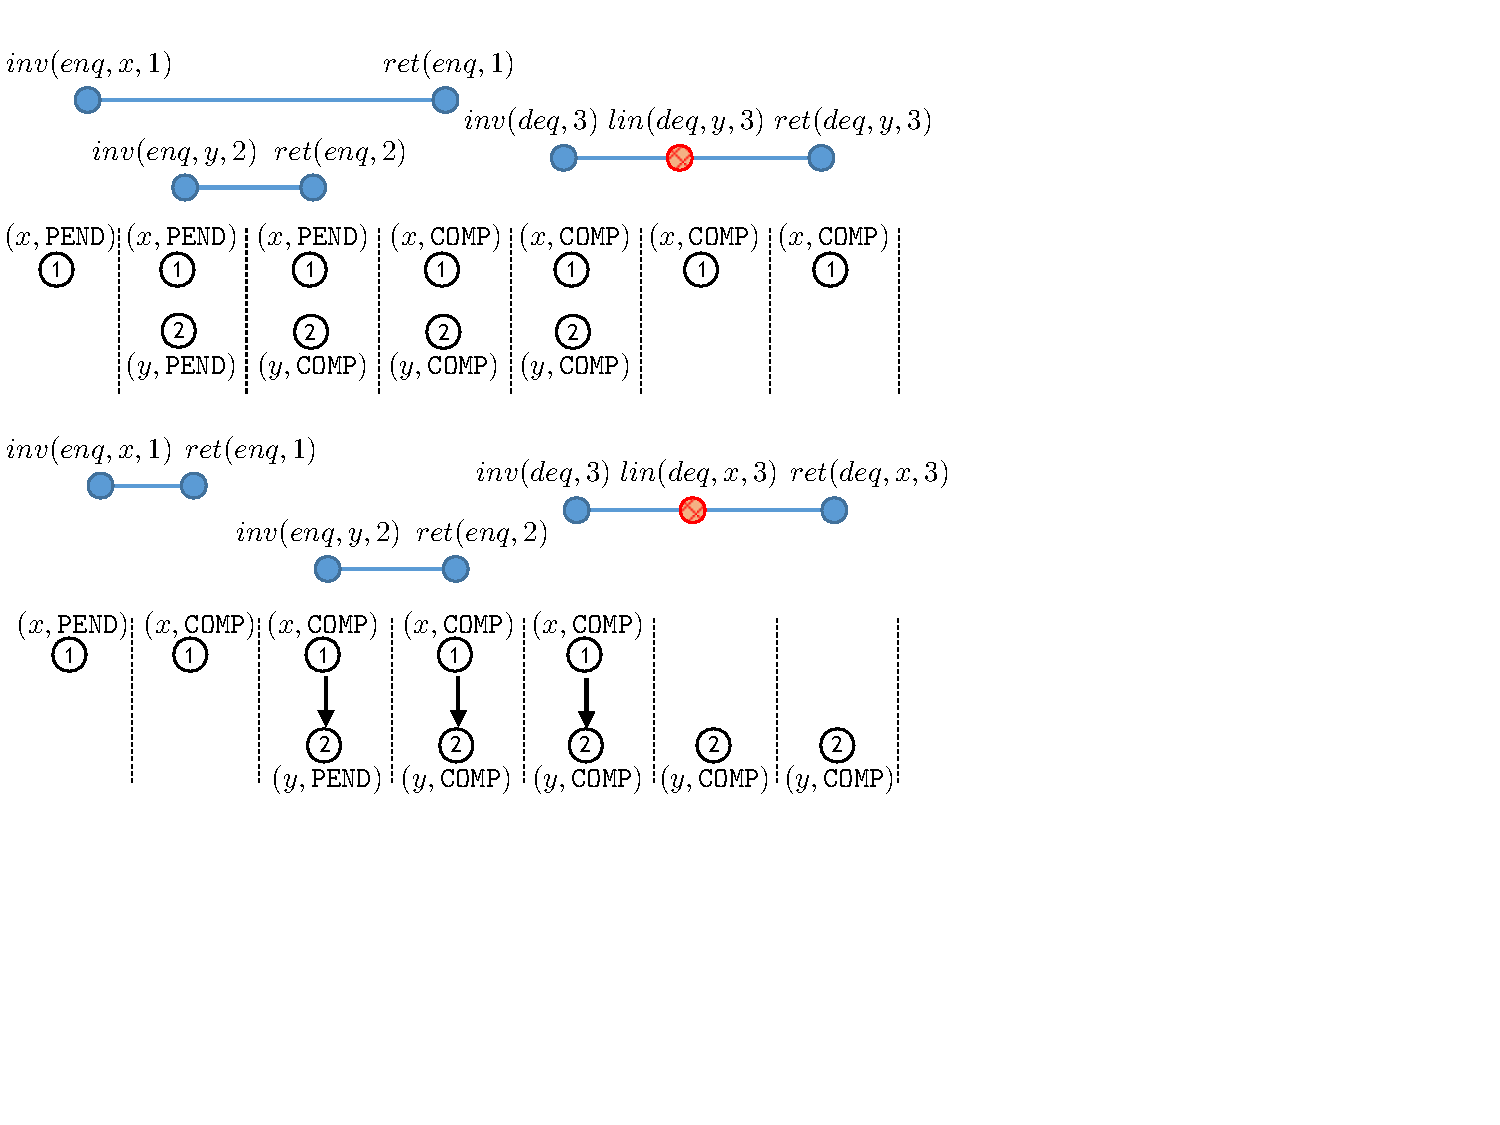
\includegraphics[width=7cm]{fig-queue12.pdf}
%
%\vspace{2mm}
%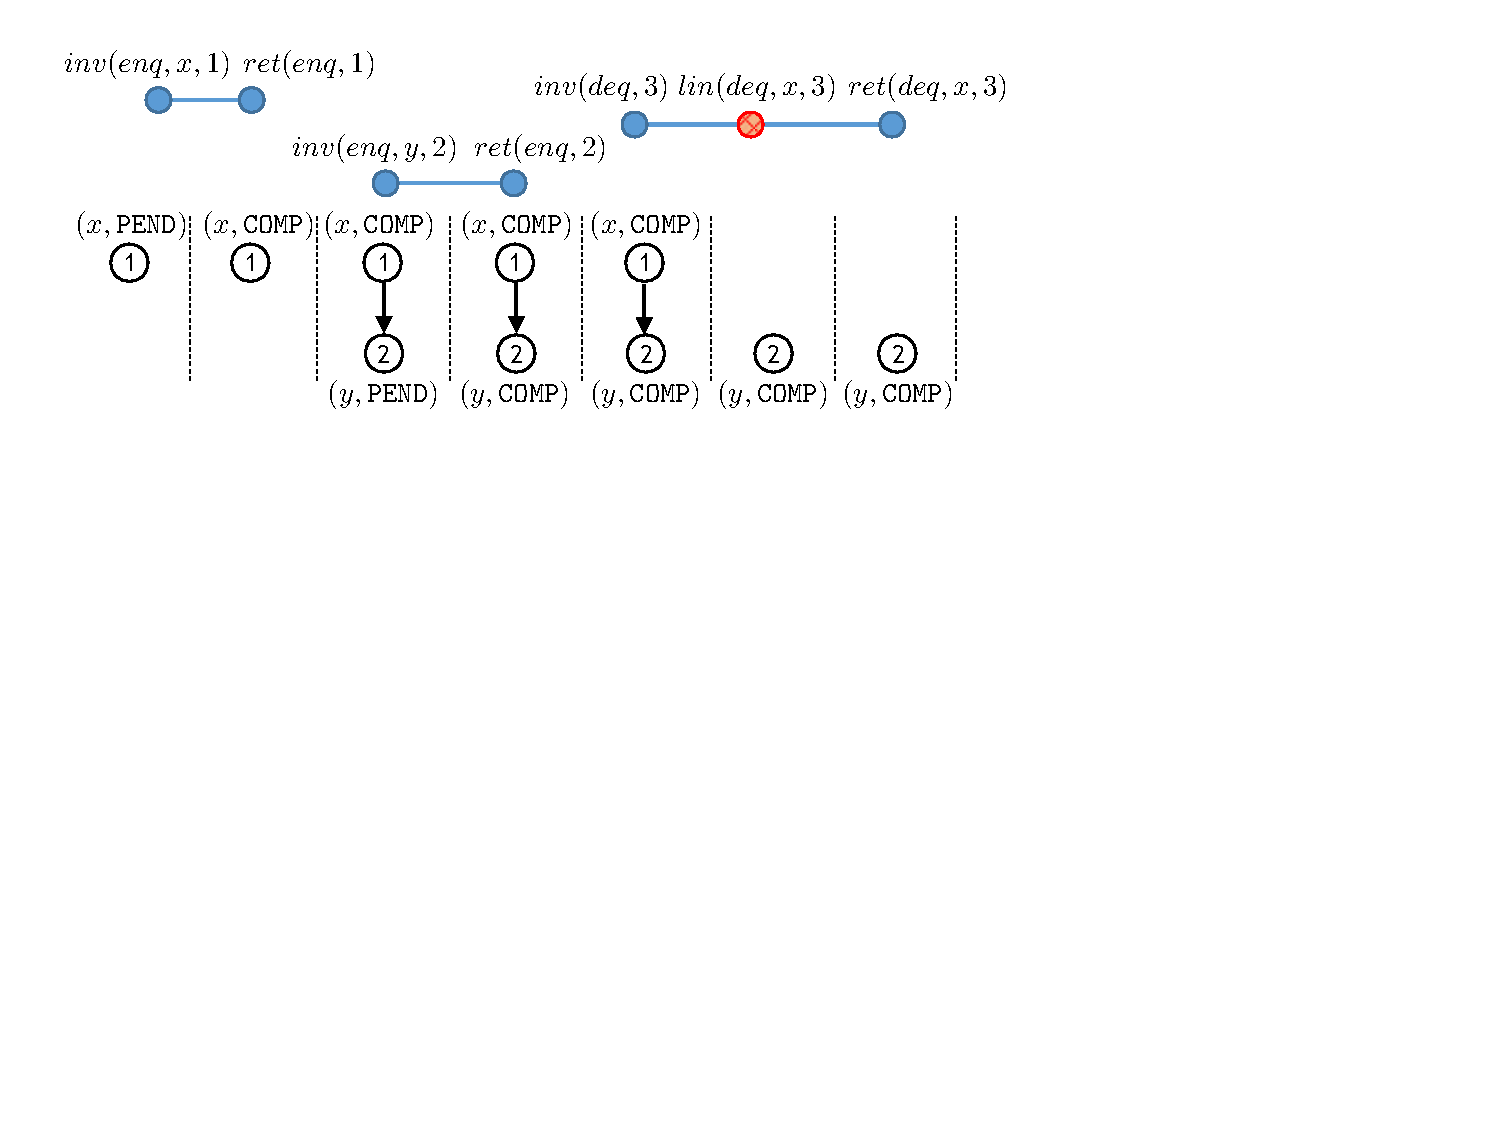
\includegraphics[width=7cm]{fig-queue2.pdf}
\vspace{-5mm}
\caption{Simulating queue histories with $AbsQ$. The order between actions is from left to right.}
\label{fig:queueSim}
\vspace{-10mm}
\end{wrapfigure}
Figure~\ref{fig:queueSim} pictures two executions of $AbsQ$ for two extended histories (that include dequeue linearization points). The state of $AbsQ$ after each action is pictured as a graph below the action. The nodes of this graph represent enqueue operations and the edges happens-before constraints. Each node is labeled by a value (the input of the enqueue) and a flag {\tt PEND} or {\tt COMP} showing whether the operation is pending or completed. For instance, in the case of the first history, the dequeue linearization point $lin(deq,y,3)$ is enabled because the current happens-before contains a \emph{minimal} enqueue operation with input $y$. Note that a linearization point $lin(deq,x,3)$ is also enabled at this state.

Formally, the states of $AbsQ$ are tuples $\tup{O,<,\ell,rv,cp}$ where $O\subseteq \<Ops>$ represents a set of operation identifiers (of previously invoked enqueue operations), $<\subseteq O\times O$ is a strict partial order, $\ell: O -> \<Vals>\times\{\tt{PEND,\tt{COMP}}\}$ labels every identifier with a value and a flag that records whether the operation is pending or completed (this flag is used to track the happens-before order), $rv:\<Ops> ~> \<Vals>$ records the return value of a pending dequeue fixed at its linearization point ($~>$ denotes a partial function), and $cp:\<Ops> ~> \{A_1,A_2,R_1,R_2,R_3\}$ records the control point of every enqueue ($A_1, A_2$) or dequeue ($R_1,R_2,R_3$) operation.
The initial state has all these components set to $\emptyset$ and the transition relation $->$ is defined in Fig.~\ref{fig:transitions:AbsQ}. The alphabet of $AbsQ$ contains call/return actions and dequeue linearization points. The latter are denoted by $lin(deq,d,k)$ where $d\in \<Vals>$, $k\in\<Ops>$. $Lin(deq)$ is the set of all such actions.

Concerning enqueue operations, the rule {\sc call-enq} orders the invoked operation after all the completed enqueue operations stored in the current state, and the rules {\sc ret-enq1}/{\sc ret-enq2} flip the corresponding flag from {\tt PEND} to {\tt COMP} provided that the operation is still present in the current state. For dequeue operations, {\sc call-deq} has no effect other than incrementing the control point and {\sc ret-deq} checks whether the return value is the same as the one fixed at the linearization point. The linearization point rule {\sc lin-deq1} corresponds to the case of a non-empty queue, showing that $lin(deq,d,k)$ is enabled only if the value $d$ has been added by an enqueue which is minimal in the current happens-before order. When it is enabled, it removes the enqueue adding $d$ from the state. The linearization point rule {\sc lin-deq2} corresponds to the case of dequeue operations linearized with an {\tt EMPTY} return value.

\begin{figure} [t]
{\scriptsize
  \centering
  \begin{mathpar}
    \inferrule[call-enq]{
      k\not\in dom(cp) \\ 
      d\neq {\tt EMPTY}
    }{
      O,<,\ell,rv,cp
      \xrightarrow{inv(enq,d,k)}
      %O\cup\{k\},<\cup \{(k',k): \ell_2(k')={\tt COMP}\},\ell[k\mapsto (d,{\tt PEND})],rv,cp[k\mapsto 1]
      O\cup\{k\},<\cup\ {\tt COMP}(O)\times\{k\},\ell[k\mapsto (d,{\tt PEND})],rv,cp[k\mapsto A_1]
    }\hspace{5mm}

    \inferrule[call-deq]{
      k\not\in dom(cp) \\ 
    }{
      O,<,\ell,rv,cp
      \xrightarrow{inv(deq,k)}
      O,<,\ell,rv,cp[k\mapsto R_1]
    }\hspace{5mm}
    \inferrule[ret-deq]{
       cp(k) = R_2 \\
       rv(k)=d  
    }{
      O,<,\ell,rv,cp
      \xrightarrow{ret(deq,d,k)}
      O,<,\ell,rv,cp[k\mapsto R_3]
    }\hspace{5mm}

    \inferrule[ret-enq1]{
      cp(k) = A_1 \\
      k \in O \\
      \ell(k) = (d,{\tt PEND}) 
    }{
      O,<,\ell,rv,cp
      \xrightarrow{ret(enq,k)}
      O,<,\ell[k\mapsto (d,{\tt COMP})],rv,cp[k\mapsto A_2]
    }\hspace{5mm}
    \inferrule[ret-enq2]{
      cp(k) = A_1 \\
      k \not\in O 
    }{
      O,<,\ell,rv,cp
      \xrightarrow{ret(enq,k)}
      O,<,\ell,rv,cp[k\mapsto A_2]
    }\hspace{5mm}

    \inferrule[lin-deq1]{
       cp(k) = R_1 \\
       d\neq{\tt EMPTY} \\
       k'\in min(O) \\ 
       \ell_1(k')=d
    }{
      O,<,\ell,rv,cp
      \xrightarrow{lin(deq,d,k)}
      O\setminus \{k'\},<\uparrow k',\ell,rv[k\mapsto d],cp[k\mapsto R_2]
    }\hspace{5mm}
    \inferrule[lin-deq2]{
       cp(k) = R_1 \\
       \forall o\in O. \ell_2(o)={\tt EMPTY}
    }{
      O,<,\ell,rv,cp
      \xrightarrow{lin(deq,{\tt EMPTY},k)}
      O,<,\ell,rv[k\mapsto {\tt EMPTY}],cp[k\mapsto R_2]
    }\hspace{5mm}    
      \end{mathpar}
  }
 \vspace{-5mm}
  \caption{The transition relation of $AbsQ$. We use the following notations: $\ell_i(k)$ denotes the projection of $\ell(k)$ over the $i$-th component, for each $i\in\{1,2\}$, ${\tt COMP}(O)=\{k\in O: \ell_2(k)={\tt COMP}\}$, $\mathit{f}[x\mapsto y]$ is the function $g$ such that $g(z)=f(z)$ for all $z\neq x$ in the domain of $f$, and $g(x)=y$, $min(O)$ is the set of elements of $O$ which are minimal in the order relation $<$, and $<\uparrow k$ denotes the relation $<$ where all the pairs containing $k$ have been removed.
  %\textcolor{red}{Call-Enq must have $d!= \texttt{EMPTY}$ as a premise. Also lin deq returning empty must be changed as before.}
  }
  \label{fig:transitions:AbsQ}
\vspace{-6mm}
\end{figure}

Both methods have a fixed linearization point when the update of the shared sequence happens. Let $AbsQ_0$ denote this implementation~\footnote{For $\<Methods>=\{enq,deq\}$, the alphabet of $AbsQ_0$ is $C\cup R\cup Lin$.} (formally defined in Appendix~\ref{app:absImplQueue}).
The following result states that the library $AbsQ$ has exactly the same set of histories as the standard abstract library $AbsQ_0$ (see Appendix~\ref{app:absImplQueue} for a proof).

\begin{theorem}\label{th:absImplQueue}
$AbsQ$ is a refinement of $AbsQ_0$ and vice-versa.
\end{theorem}

A trace of a queue implementation is called \emph{$Lin(deq)$-complete} when every completed dequeue has a linearization point, i.e., TODO. A queue implementation $L$ over alphabet $\Sigma$ is called \emph{with fixed dequeue linearization points} if{f} $C\cup R\cup Lin(deq)\subseteq \Sigma$ 
and every trace $@t\in Tr(L)$ is $Lin(deq)$-complete.

TODO NEEDS DATA INDEPENDENCE FOR THE LINEARIZATION POINT TRANSITIONS TO BE DETERMINISTIC

The following result shows that $C\cup R\cup Lin(deq)$-forward simulations are a sound and complete proof method for showing the correctness of a queue implementation with fixed dequeue linearization points (up to the correctness of the linearization points). It is obtained from Theorem~\ref{th:absImplQueue} and Theorem~\ref{th:forSim} using the fact that the alphabet of $AbsQ$ is exactly $C\cup R\cup Lin(deq)$ and $AbsQ$ is deterministic.

\begin{corollary}
A queue implementation $L$ with fixed dequeue linearization points is a $C\cup R\cup Lin(deq)$-refinement of $AbsQ_0$ if{f} there exists a $C\cup R\cup Lin(deq)$-forward simulation from $L$ to $AbsQ$.
\end{corollary}

\subsection{A Correctness Proof For Herlihy\&Wing Queue}\label{ssec:HerlihyWing}

We describe a forward simulation $\mathit{fs}$ from $\mathit{HWQ}$ to $AbsQ$. Essentially, an $AbsQ$ state associated by $\mathit{fs}$ to a $\mathit{HWQ}$ state consists of all the  enqueue operations for which the input is still present in the array {\tt items} and all the pending enqueue operations that have at most reserved an array position, ordered by a relation $<$ satisfying the following: 
\begin{itemize}
	\item[(a)] pending enqueues are maximal, i.e., for every two enqueues $k$ and $k'$ such that $k'$ is pending, we have that $k'\not< k$,
	\item[(b)] $<$ is consistent with the order in which positions of {\tt items} have been reserved, i.e., for every two enqueues $k$ and $k'$ such that ${\tt i}(k) < {\tt i}(k')$, we have that $k' \not< k$,
	\item[(c)] an enqueue which has reserved an array position $i$ %and executed only the first statement 
	can't be ordered before another enqueue that has reserved a position $j \geq i$ when the position $i$ has been ``observed'' by a non-linearized dequeue that may ``observe'' $j$ in the current array traversal, i.e., for every two enqueues $k$ and $k'$, and a dequeue $k_d$, such that 
	
	\noindent
	{\small
	\begin{align}
	\hspace{-8mm}
	{\tt x}(k_d)={\tt null} \land {\tt i}(k') \leq {\tt range}(k_d) \land {\tt i}(k) \leq {\tt i}(k_d) \leq {\tt i}(k')
	 \land ({\tt i}(k) = {\tt i}(k_d) => k_d\atCP {\tt if}\text{-}{\tt inc}) \label{eq:inst}
	\end{align}}
	
	\noindent
	we have that $k \not< k'$. The predicate $k_d\atCP {\tt if}\text{-}{\tt inc}$ holds when the dequeue $k_d$ is at a control point after a {\tt swap} returning {\tt null} and before the increment of {\tt i}.
\end{itemize}

An enqueue is labeled by $(d,{\tt PEND})$ where $d$ is the input value if it's pending and by  $(d,{\tt COMP})$, otherwise. Also, for every dequeue operation $k$ such that ${\tt x}(k)=d\neq {\tt null}$, we have that $rv(k)=d$.

We show that $\mathit{fs}$ is indeed a $C\cup R\cup Lin(deq)$-forward simulation. Let $s$ and $t$ be states of $\mathit{HWQ}$ and $AbsQ$, respectively, such that $(s,t)\in\mathit{fs}$. 
We omit discussing the trivial case of transitions labeled by call and return actions which are simulated by similar transitions of $AbsQ$ (for the return a dequeue operation $k$, we use the equality between the local variable ${\tt x}(k)$ in $s$ and the component $rv(k)$ in $t$). 
%\textcolor{red}{ I think it is good to mention again that call/return actions in HWQ correspond to the same call/return actions in AbsQ (without any other internal action). I also think that invoke enqueue operation is non-trivial. Preservation of the strict partial order and all of the above items a, b and c needs to be rechecked.}

We show that each internal step of an enqueue or dequeue, except the execution of {\tt swap} returning a non-null value in dequeue (which represents its linearization point), is simulated by an \emph{empty} sequence of $AbsQ$ transitions, i.e., for every state $s'$ obtained through one of these steps, if $(s,t)\in\mathit{fs}$, then $(s',t)\in\mathit{fs}$ for each $AbsQ$ state $t$. We focus on the following essential property, called \emph{monotonicity}: the set of possible orders $<$ associated by $\mathit{fs}$ to $s'$ doesn't exclude any order $<$ associated to $s$.
%Essentially, this boils down to showing that the constraints over $<$ in the definition of $\mathit{fs}$ are an invariant for these steps.

Concerning enqueues, let $s'$ be the state obtained from $s$ when a pending enqueue $k$ reserves an array position. This enqueue operation must be maximal in both $t$ and any state $t'$ related to $s'$ (because it is pending). Moreover, there is no dequeue that can ``observe'' this position before restarting the array traversal. Therefore, item (c) in the definition of $<$ doesn't constrain the order between $k$ and some other enqueue neither in $s$ nor in $s'$. Since this transition doesn't affect the constraints on the order between enqueue operations different from $k$ (their local variables remain unchanged), we have that monotonicity holds. This property is trivially satisfied by the second step of enqueue which doesn't affect {\tt i}.

To prove monotonicity in the case of dequeue internal steps different from its linearization point, it is important to track the non-trivial instantiations of item (c) in the definition of $<$ over the two states $s$ and $s'$., i.e., the triples $(k,k',k_d)$ for which (\ref{eq:inst}) holds. Instantiations that are enabled only in $s'$ may in principle lead to a violation of monotonicity (since they restrict the orders $<$ associated to $s'$). For the two steps that begin an array traversal, i.e., reading the index of the last used position and setting the iterator {\tt i} to $0$, there exist no  such new instantiations in $s'$ because the value of {\tt i} is either not set or $0$. % (it is trivial to notice that applying these steps doesn't disable such instantiations that were possible in $s$). 
%The same holds for the step incrementing the iterator {\tt i}. 
%
%The execution of {\tt swap} returning {\tt null} may introduce one new non-trivial instantiation $(k,k',k_d)$ of item (c).
%We write ${\tt i}_s(k)$ to refer to the value of the variable {\tt i} of operation $k$ in state $s$. Assume that indeed, there exist two enqueue operations $k$ and $k'$ such that ${\tt i}_{s'}(k) < {\tt i}_{s'}(k_d) \leq {\tt i}_{s'}(k')$, ${\tt x}_{s'}(k_d)={\tt null}$, ${\tt i}_{s'}(k') \leq {\tt range}_{s'}(k_d)$ TODO SWAP. Since {\tt swap} returnes {\tt null}, the position ${\tt i}_{s'}(k_d)$
%
%
% and ${\tt i}_{s}(k) = {\tt i}_{s'}(k_d)$. The latter constraint guarantees that this instantiation is not enabled in state $s$. The increment of {\tt i} being enabled, implies that 
%
The same is true for the increment of the iterator {\tt i} in a dequeue $k_d$ since the predicate $k_d\atCP {\tt if}\text{-}{\tt inc}$ holds in state $s$.
The execution of {\tt swap} returning {\tt null} in a dequeue $k_d$ enables new instantiations $(k,k',k_d)$ in $s'$, thus adding potentially new constraints $k\not< k'$. We show however that these instantiations are vacuous because $k$ must be a pending enqueue in $s$ and thus maximal in any order relation $<$ associated by $\mathit{fs}$ to $s$.
Let $k$ and $k'$ be two enqueue operations such that together with the dequeue $k_d$ they satisfy the property (\ref{eq:inst}) in $s'$ but not in $s$. 
We write ${\tt i}_s(k)$ to refer to the value of the variable {\tt i} of operation $k$ in state $s$. 
This implies that ${\tt i}_{s'}(k) = {\tt i}_{s'}(k_d) \leq {\tt i}_{s'}(k')$ and ${\tt items}[{\tt i}_{s'}(k_d)]={\tt null}$. The latter implies that the enqueue $k$ didn't executed
the second statement and it is pending (because the position it reserved is still {\tt null}). Finally, checking whether the value returned by {\tt swap} is {\tt null} doesn't modify any of the variables in property  (\ref{eq:inst}) and also, it doesn't change the valuation of the predicate $\atCP {\tt if}\text{-}{\tt inc}$.

Finally, we show that the linearization point of a dequeue $k$ of $\mathit{HWQ}$, i.e., an execution of {\tt swap} returning a non-null value $d$, from state $s$ and leading to a state $s'$ is simulated by a transition labeled by $lin(deq,d,k)$ of $AbsQ$ from state $t$. By the definition of $\mathit{HWQ}$, there exists a unique enqueue $k_e$ which filled the position updated by $k$, i.e., ${\tt i}_s(k_e)=i_s(k)$ and ${\tt x}_{s'}(k)={\tt x}_s(k_e)$. We show that $k_e$ is minimal in the order relation $<$ of $t$ which implies that $lin(deq,d,k)$ is enabled in $t$. Thus, instantiating item (c) in the definition of $<$ with $k'=k_e$ and $k_d=k$ we get that every enqueue that reserved a position smaller than the one of $k_e$ can't be ordered before $k_e$ in the order $<$. Also, applying item (b) with $k=k_e$ we get the same for every enqueue that reserved a bigger position. An enqueue that didn't reserved a position is by definition maximal in the order $<$ and therefore, not a predecessor of $k_e$. The state $t'$ obtained from $t$ through a $lin(deq,d,k)$ transition is related to $s'$ because essentially, (1) the value added by $k_e$ is not anymore present in {\tt items} which implies that $k_e$ doesn't occur in any $AbsQ$ state related to $s'$, and (2) the value of ${\tt x}(k)$ is set to $d\neq {\tt null}$ which implies that $rv(k)$ is set to $d$ in every $AbsQ$ state related to $s'$.

%\section{Existence of Forward Simulations for Stack Implementations that have Fixed Pop Linearization Points}
%!TEX root = draft.tex
\vspace{-3.5mm}
\section{Stacks With Fixed Pop Commit Points}\label{sec:stacks}
\vspace{-1.5mm}
The abstract implementation in Section~\ref{sec:queues} can be adapted to stacks, the main modification being that the linearization point $lin(pop,d,k)$ with $d\neq{\tt EMPTY}$ is enabled when $k$ is added by a push which is maximal in the happens-before order stored in the state. However, there are stack implementations, e.g., Time-Stamped Stack~\cite{DBLP:conf/popl/DoddsHK15} ($\mathit{TSS}$, for short), which cannot be proved correct using forward simulations to this abstract implementation because the linearization points of the pop operations are not fixed.
%this stack implementation cannot simulate (through forward simulations) existing stack implementations like the Time-Stamped Stack~\cite{DBLP:conf/popl/DoddsHK15} ($\mathit{TSS}$, for short) where the linearization points of the pop operations are not fixed.
Exploiting particular properties of the stack semantics, we refine the ideas used in $AbsQ$ and define
a new abstract implementation for stacks, denoted as $AbsS$, which is able to simulate such implementations. Forward simulations to $AbsS$ are complete for proving the correctness of stack implementations provided that the point in time where the return value of a pop operation is determined, called \emph{commit point}, corresponds to a fixed statement in the pop method.
% provided that the point in time where the return value of a pop operation is determined corresponds to a fixed action. To demonstrate the use of this abstract implementation we provide a correctness proof for a simplified version of Time-Stamped Stack that preserves its most complex behaviors.

\vspace{-3.5mm}
\subsection{Pop Methods With Fixed Commit Points}
\vspace{-1mm}

We explain the meaning of the commit points on a simplified version of the Time-Stamped Stack~\cite{DBLP:conf/popl/DoddsHK15} ($\mathit{TSS}$, for short) given in Fig.~\ref{fig:TimeStamped}. This  implementation maintains an array of singly-linked lists, one for each thread, where list nodes contain a data value (field {\tt data}), a timestamp (field {\tt ts}), the next pointer (field {\tt next}), and a Boolean flag indicating whether the node represents a value removed from the stack (field {\tt taken}). Initially, each list contains a sentinel dummy node pointing to itself with timestamp $-1$ and the flag {\tt taken} set to {\tt false}.


\begin{figure}[t]
  \begin{minipage}[t]{0.49\linewidth}
    \begin{lstlisting}
struct Node{
  int data;
  int ts;
  Node* next;
  bool taken;
};

bool CAS(bool data, bool a, bool b);

Node* pools[maxThreads];
int TS = 0;

void push(int x) {
  Node* n =
    new Node(x,MAX_INT, null,false);
  n->next = pools[myTID];
  pools[myTID] = n;
  int i = TS++;
  n->ts = i;
}
    \end{lstlisting}
  \end{minipage}
  \hfill
  \begin{minipage}[t]{0.49\linewidth}
    \begin{lstlisting}
int pop() {
  bool success = false;
  int maxTS = -1;
  Node* youngest = null;
  while ( !success ) {
    maxTS = -1; youngest = null;
    for(int i=0; i<maxThreads; i++) {
      Node* n = pools[i];
      while (n->taken && n->next != n)
        n = n->next;
      if(maxTS < n->ts) {
        maxTS = n->ts; youngest = n;
      }
    }
    if (youngest != null)
      success =
        CAS(youngest->taken, false, true);
  }
  return youngest->data;
}
    \end{lstlisting}
  \end{minipage}

  \caption{The Time-Stamped Stack~\cite{DBLP:conf/popl/DoddsHK15}.}
  \label{fig:TimeStamped}
\end{figure}

Pushing a value to the stack proceeds in several steps: adding a node with maximal timestamp in the list associated to the thread executing the push (given by the special variable {\tt myTID}), asking for a new timestamp (given by the shared variable {\tt TS}), and updating the timestamp of the added node. Popping a value from the stack consists in traversing all the lists, finding the first element which doesn't represent a removed value (i.e., {\tt taken} is {\tt false}) in each list, and selecting the element with the maximal timestamp. A compare-and-swap (CAS) is used to set the {\tt taken} flag of this element to {\tt true}. The procedure restarts if the CAS fails.

\begin{figure}[t]
\centering
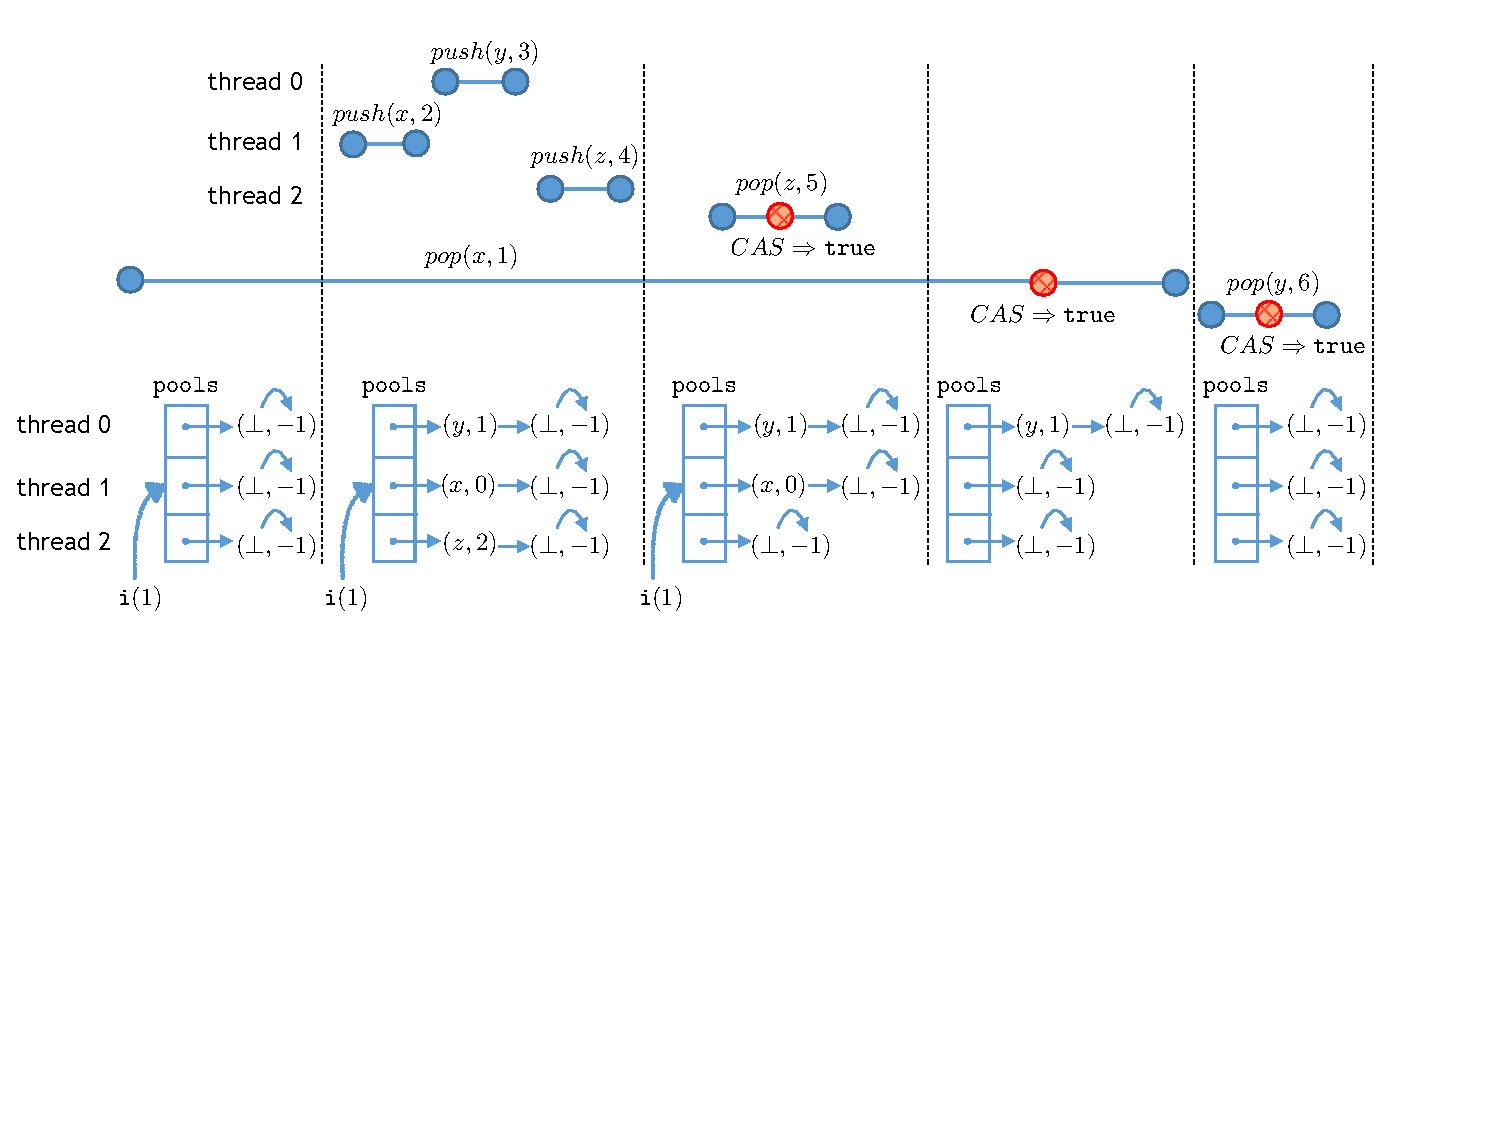
\includegraphics[width=11.5cm]{fig-tss.pdf}
\vspace{-4mm}
\caption{An execution of $\mathit{TSS}$. An operation is pictured by a line delimited by two circles denoting the call and respectively, the return action. Pop operations with identifier $k$ and removing value $d$ are labeled $pop(d,k)$. Their representation includes another circle that stands for a successful CAS which is their commit point. The library state after an execution prefix delimited at the right by a dotted line is pictured in the bottom part (the picture immediately to the left of the dotted line). A pair $(d,t)$ represents a list node with ${\tt data}=d$ and ${\tt ts}=t$, and ${\tt i}(1)$ denotes the value of {\tt i} in the pop with identifier 1. We omit the nodes where the field {\tt taken} is {\tt true}.}
\label{fig:commit}
\vspace{-6mm}
\end{figure}


The push operations don't have a fixed linearization point because adding a node to a list and updating its timestamp are not executed in a single atomic step. The nodes can be added in an order which is not consistent with the order between the timestamps assigned later in the execution. Also, the value added by a push that just added an element to a list can be popped before the value added by a completed push (since it has a maximal timestamp). The same holds for pop operations: The only reasonable choice for a linearization point is a successful CAS (that results in updating the field {\tt taken}). Fig.~\ref{fig:commit} pictures an execution showing that this action doesn't correspond to a linearization point, i.e., an execution for which the pop operations in every correct linearization are not ordered according to the order between successful CASs. In every correct linearization of that execution, the pop operation removing $x$ is ordered before the one removing $z$ although they perform a successful CAS in the opposite order.

An interesting property of the successful CASs in pop operations is that they fix the return value, i.e., the return value is {\tt youngest->data} where {\tt youngest} is the node updated by the CAS. We call such actions \emph{commit points}. More generally, commit points are actions that access shared variables, from which every control-flow path leads to the return control point and contains no more accesses to the shared memory (i.e., after a commit point, the return value is computed using only local variables).

%The complete version of $\mathit{TSS}$~\cite{DBLP:conf/popl/DoddsHK15} contains also a mechanism for elimination (a pop can remove a value without traversing all the lists if it has been added by a concurrent push) and emptiness checking. In both cases, the commit points can be identified in the code and correspond to certain boolean conditions evaluated to {\tt true}.

%TODO WHAT CAN WE SAY ABOUT COMMIT POINTS IN OTHER IMPLEMENTATIONS

%Usually, a stack implementation stores the pushed values into a data structure, e.g., a singly-linked list, and a pop operation contains an action (typically, a compare-and-swap) that removes an element from this data structure (or sets a flag associated to this element to a ``deleted'' state). Such an action represents a commit point since the pop operation will return the value stored in this element.


%TODO GIVE AN EXAMPLE TO SHOW THE ISSUE WITH POP LINEARIZATION POINTS, AND TO SHOW THAT COMMIT POINTS ARE RIGHT LIMITS FOR THE INTERVAL OF A LIN POINT, I.E., A POP WITH A LATER COMMIT POINT CAN BE LINEARIZED BEFORE. NEED ONLY 2 POPS IN AN EXECUTION

When the commit points of pop operations are fixed to particular implementation actions (e.g., a successful CAS) we assume that the library is an LTS over an alphabet that contains actions $com(pop,d,k)$ with $d\in\<Vals>$ and $k\in\<Ops>$ (denoting the commit point of the pop with identifier $k$ and returning $d$). Let $Com(pop)$ be the set of such actions.
%We consider a set of actions $Com(pop)=\set{com(pop,d,k):d\in\<Vals>, k\in\<Ops>}$, called \emph{commit points}, representing actions of a pop operation where its return value is determined.
%TODO DESCRIBE THE TIME-STAMPED STACK, EXPLAIN THAT NO METHOD HAS A FIXED LIN POINT, GIVE THE COMMIT POINTS, SHOW THAT COMMIT POINTS ARE NOT LIN POINTS
%
%COMMIT POINTS ARE LINEARIZATION POINTS WHEN THE LIBRARY IS INTERPRETED AS A MULTISET

\vspace{-3mm}
\subsection{Abstract stack implementation}
\vspace{-1mm}
We define an abstract stack $AbsS$ over alphabet $C\cup R\cup Com(pop)$ that essentially, similarly to $AbsQ$, maintains the happens-before order of the pushes whose value has not yet been  removed by a matching pop. Pop operations are treated differently since the commit points are not necessarily linearization points. Intuitively, a pop can be linearized before its commit point. Each pop operation starts by taking a snapshot of the completed push operations which are maximal in the happens-before, more precisely, which don't happen before another completed push operation. Also, the library maintains the set of push operations overlapping with each pop operation. The commit point $com(pop,d,k)$ with $d\neq {\tt EMPTY}$ is enabled if either $d$ was added by one of the push operations in the initial snapshot, or by a push happening earlier when arguments of pushes from the initial snapshot have been removed, or by one of the push operations that overlaps with pop $k$. The commit point $com(pop,{\tt EMPTY},k)$ is enabled if all the values added by push operations happening before $k$ have been removed. The effect of the commit points is explained below through examples.
\vspace{-.4mm}

%\begin{wrapfigure}{l}{7.8cm}
%\vspace{-6mm}
\begin{figure}[t]
\centering
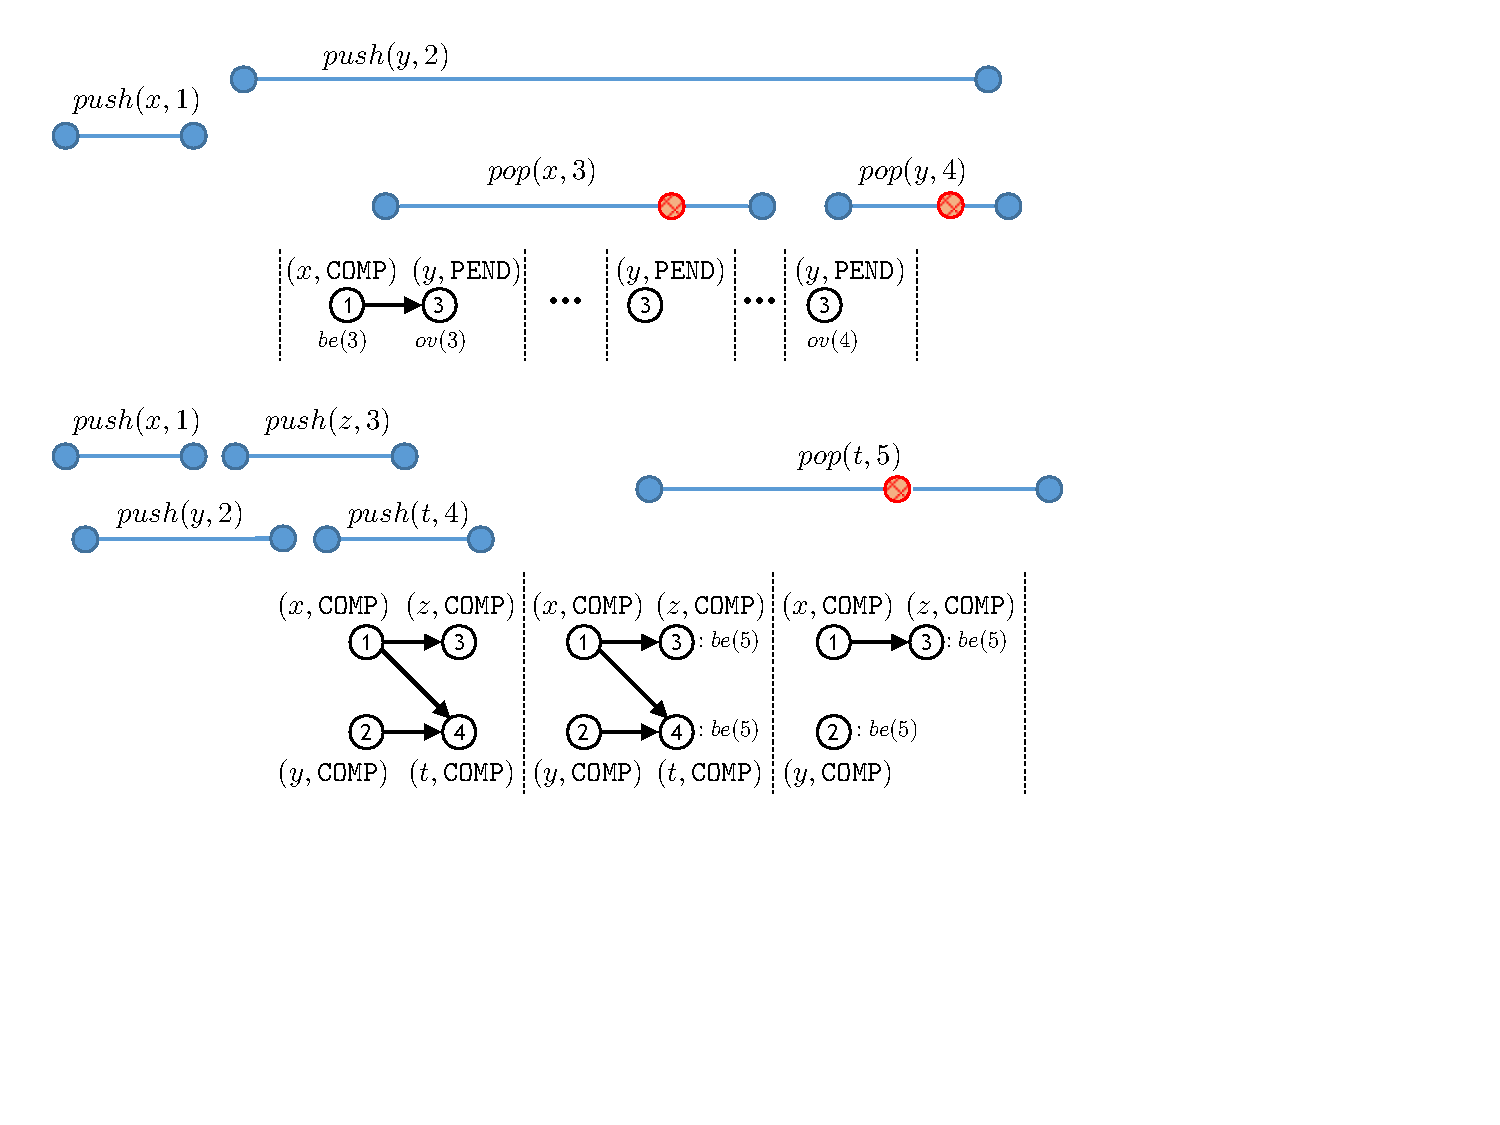
\includegraphics[width=10cm]{fig-stack.pdf}
%
%\vspace{2mm}
%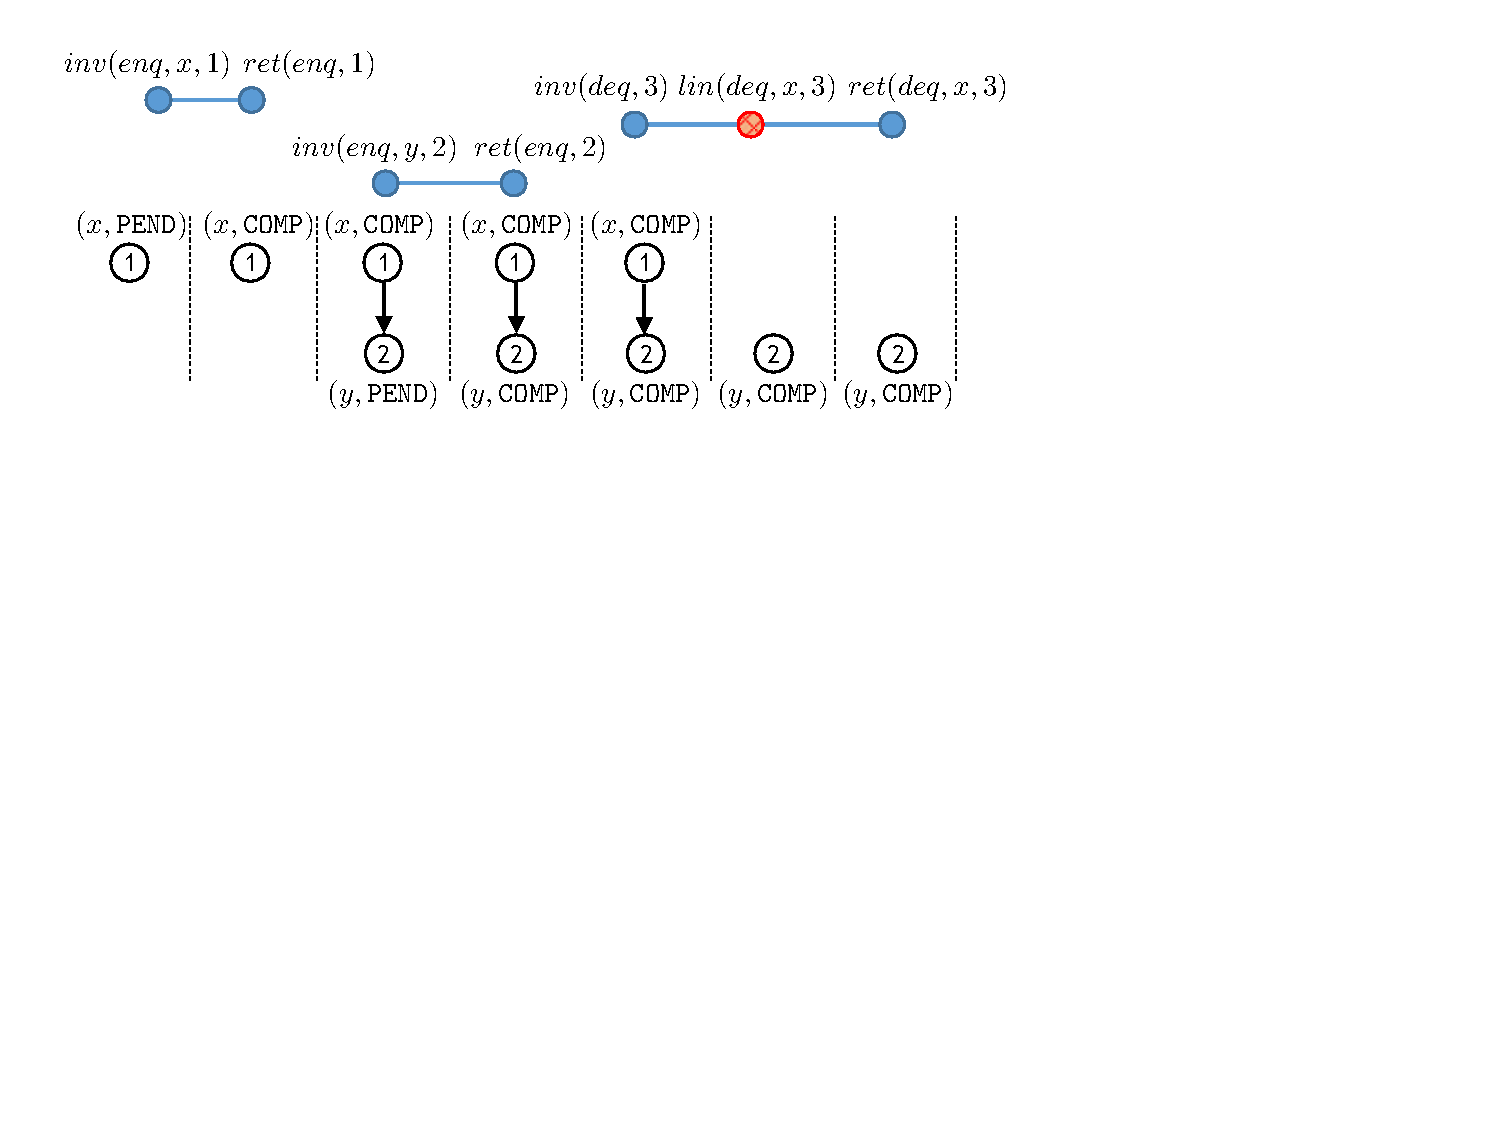
\includegraphics[width=7cm]{fig-queue2.pdf}
\vspace{-2mm}
\caption{Simulating stack histories with $AbsS$.}
\label{fig:stackSim}
\vspace{-6.5mm}
\end{figure}

Fig.~\ref{fig:stackSim} pictures two executions of $AbsS$ for two extended histories (that include pop commit points). For readability, we give the state of $AbsS$ only after several execution prefixes delimited at the right by a dotted line. We focus on pop operations -- the effect of push calls and returns is similar to enqueue calls and returns in $AbsQ$. Let us first consider the history on the top part. The first state we give is reached after the call of pop with identifier $3$. This shows the effect of a pop invocation: the greatest completed pushes according to the current happens-before (here, the push with identifier $1$) are marked as $\mathsf{maxAtInvoc}(3)$, and the pending pushes are marked as $\mathsf{overlap}(3)$. As a side remark, any other push operation that starts after pop $3$ would be also marked as $\mathsf{overlap}(3)$.
The commit point $com(pop,x,3)$ (pictured with a red circle) is enabled because $x$ was added by a push marked as $\mathsf{maxAtInvoc}(3)$. The effect of the commit point is that push $1$ is removed from the state (the execution on the bottom shows a more complicated case). For the second pop, the commit point $com(pop,y,4)$ is enabled because $y$ was added by a push marked as $\mathsf{overlap}(4)$. The execution on the bottom shows an example where the marking $\mathsf{maxAtInvoc}(k)$ for some pop $k$ is updated at commit points. The pushes $3$ and $4$ are marked as $\mathsf{maxAtInvoc}(5)$ and $\mathsf{maxAtInvoc}(6)$
when the pops $5$ and $6$ start. Then, $com(pop,t,5)$ is enabled since $t$ was added by $push(t,4)$ which is marked as $\mathsf{maxAtInvoc}(5)$. Besides removing $push(t,4)$, the commit point produces a state where a pop committing later, e.g., pop $6$, can remove $y$ which was added by a predecessor of $push(t,4)$ in the happens-before ($y$ could become the top of the stack when $t$ is removed). This history is valid because $push(y,2)$ can be linearized after $push(x,1)$ and $push(z,3)$. Thus, push 2, a predecessor of the push which is removed, is marked as $\mathsf{maxAtInvoc}(6)$. Push $1$ which is also a predecessor of the removed push is not marked as $\mathsf{maxAtInvoc}(6)$ because it happens before another push, i.e., push 3, which is already marked as $\mathsf{maxAtInvoc}(6)$ (the value added by push 3 should be removed before the value added by push 1 could become the top of the stack).

\begin{figure}[t]
  \begin{minipage}[t]{0.39\linewidth}
    \begin{lstlisting}
function loc: $\mathbb{O} \to \set{\tt inv, com, ret, \bot}$
function arg, ret: $\mathbb{O} \to \mathbb{V}$
function present, pending: $\mathbb{O} \to \mathbb{B}$
function before: $\mathbb{O} \times \mathbb{O} \to \mathbb{B}$
function maxAtInvoc: $\mathbb{O} \to \pow{\mathbb{O}}$
function overlap: $\mathbb{O} \to \pow{\mathbb{O}}$

rule inv(push,x,k):
  present(k) := true
  pending(k) := true
  arg(k) := x
  forall k1 with present(k1):
    if $\lnot$pending(k1):
      before(k1,k) := true
  forall k1 with pending(k1):
    overlap(k1) := overlap(k1)$\cup$$\{$k$\}$

rule ret(push,k):
  pending(k) := false

rule ret(pop,y,k):
  assert ret(k) = y
    \end{lstlisting}
  \end{minipage}
  \begin{minipage}[t]{0.59\linewidth}
    \begin{lstlisting}
rule inv(pop,k):
  forall k1 with present(k1):
    if pending(k1):
      overlap(k) := overlap(k) $\cup$ $\{$k1$\}$
    else:
      if $\forall$k2.present(k2)$\land$before(k1,k2)$\Rightarrow$pending(k2):
        maxAtInvoc(k) = maxAtInvoc(k) $\cup$ $\{$k1$\}$

rule com(pop,y,k):
  ret(k) := y
  if y = EMPTY:
    assert maxAtInvoc(k) = $\emptyset$
  else:
    let k1 := arg$^{-1}$(y)
    assert present(k1)
    assert k1 $\in$ maxAtInvoc(k) $\cup$ overlap(k)
    present(k1) := false
    forall k2 with k1 $\in$ maxAtInvoc(k2):
      maxAtInvoc(k2) := maxAtInvoc(k2) $\setminus$ $\{$k1$\}$
      forall k3 with before$_1$(k3,k1):
        if $\forall$k4$\neq$k1.before$_1$(k3,k4) $\Rightarrow$ k4$\in$overlap(k2):
          maxAtInvoc(k2) := maxAtInvoc(k2) $\cup$ $\{$k3$\}$
    \end{lstlisting}
  \end{minipage}
  \caption{The $AbsS$ implementation; each rule \lstinline|$\alpha$(\_,k)|
  implicitly begins with \lstinline|assert loc(k)=$\alpha$| and ends with the
  appropriate \lstinline|loc(k):=$\beta$|; and \lstinline|before$_1$| denotes
  the transitive reduction of \lstinline|before|.}
  \label{fig:transitions:AbsS}
\end{figure}

The description of $AbsS$ as an abstract state machine is given in Fig.~\ref{fig:transitions:AbsS}. Compared to the queue implementation $AbsQ$, the shared state contains two more functions $\mathsf{maxAtInvoc}$ and $\mathsf{overlap}$. For each pop operation $k$, $\mathsf{maxAtInvoc}(k)$ records the set of completed push operations which were maximal in the happens-before (defined by $\mathsf{before}$) when pop $k$ was invoked, or happening earlier provided that the values of all the pushes happening later than one of these maximal ones and before pop $k$ have been removed. Also, for each pop operation $k$, $\mathsf{overlap}(k)$ contains the push operations overlapping with pop $k$.
%Formally, the states of $AbsS$ are tuples $\tup{O,<,\ell,rv,cp,be,ov}$ where $<$ is a strict partial order over the set $O$ of operation identifiers, $\ell: O -> \<Vals>\times\{\tt{PEND,\tt{COMP}}\}$ labels every identifier in $O$ with a value and a pending/completed flag, $rv:\<Ops> ~> \<Vals>$ records the return value of a pending pop fixed at its commit point, $cp:\<Ops> ~> \{A_1,A_2,R_1,R_2,R_3\}$ records the control point of every push ($A_1, A_2$) or pop operation ($R_1,R_2,R_3$), $be:\<Ops> ~> 2^O$ records the greatest completed push operations before a pop started or happening earlier provided that the values of all the push happening later have been removed, and $ov: \<Ops> ~> 2^O$ records push operations overlapping with a pop.
%%The initial state has all these components set to $\emptyset$ and the transition relation $->$ is defined in Figure~\ref{fig:transitions:AbsS}.
%All the components are $\emptyset$ in the initial state, and the transition relation $->$ is defined in Fig.~\ref{fig:transitions:AbsS}.
In the initial state, the domain of every function (predicate) is empty. The push methods are similar to the enqueue methods in $AbsQ$. The only difference is that every newly invoked push operation {\tt k} is added to the set $\mathsf{overlap}(${\tt k1}$)$ for all pop operations {\tt k1} (since {\tt k} overlaps with all the currently pending pops). The rule {\tt inv(pop,k)}, marking the invocation of a pop, sets $\mathsf{maxAtInvoc}(${\tt k}$)$ and $\mathsf{overlap}(${\tt k}$)$ as explained above. The rule {\tt com(pop,y,k)} results in setting the return value {\tt y} to {\tt EMPTY} if the set $\mathsf{maxAtInvoc}(${\tt k}$)$ is empty (otherwise, there would be push operations happening before pop {\tt k} which makes the answer {\tt EMPTY} incorrect). It results in setting the return value to a value $d\neq\,${\tt EMPTY} when $d$ was added by a push {\tt k1} which belongs to $\mathsf{maxAtInvoc}(${\tt k}$)$ or $\mathsf{overlap}(${\tt k}$)$. In this case, the rule {\tt com(pop,y,k)} may also update $\mathsf{maxAtInvoc}(${\tt k2}$)$ for other pending pops {\tt k2}. More precisely, whenever $\mathsf{maxAtInvoc}(${\tt k2}$)$ contains the push {\tt k1}, the latter is replaced by the immediate predecessors of {\tt k1} (according to $\mathsf{before}$) that are followed exclusively by pushes overlapping with {\tt k2}.
%The transition rules which don't correspond to commit point actions are similar to those for $AbsQ$. The rule {\sc com-pop1} for $com(pop,d,k)$ is enabled only if there exists a push $k'$ which added value $d$ and which belongs to $be(k)$ or $ov(k)$. When enabled, the push $k'$ is removed from the set $O$ (and the order $<$) and for every other pop $k_1$ such that $k'$ belongs to $be(k_1)$, $k'$ is replaced in $be(k_1)$ by its predecessors which are followed exclusively by pushes overlapping with $k_1$ (these predecessors become maximal closed pushes once $k'$ is removed). Also, $rv(k)$ is set to $d$. The rule {\sc com-pop1} for $com(pop,{\tt EMPTY},k)$ is enabled only if $be(k)$ is empty (i.e., all the values added by pushes ending before $k$, if any, have been removed). Then, $rv(k)$ is set to ${\tt EMPTY}$.

The abstract state machine in Fig.~\ref{fig:transitions:AbsS} defines an LTS over the alphabet $C\cup R\cup Com(pop)$. As in the case of $AbsQ$, we assume that the transition corresponding to the invocation, resp., the return, of a method, is done atomically with the fist, resp., the last, macro rule in its body. These transitions are labeled as expected with call and return actions (borrowing the operation identifier which occurs as argument of the macro rule), and the transitions corresponding to the rule {\tt com(pop,y,k)} are labeled by $com(pop,d,k)$.

Let $AbsS_0$ be the standard abstract implementation of a stack where elements are stored in a sequence, push and pop operations adding and removing an element from the beginning of the sequence in one atomic step, respectively. For $\<Methods>=\{push,pop\}$, the alphabet of $AbsS_0$ is $C\cup R\cup Lin$.
The following result states that the library $AbsS$ has exactly the same set of histories as $AbsS_0$.

\vspace{-2mm}
\begin{theorem}\label{th:absImplStack}
$AbsS$ is a refinement of $AbsS_0$ and vice-versa.
\vspace{-2mm}
\end{theorem}

A trace of a stack implementation is called \emph{$Com(pop)$-complete} when every completed pop has a commit point, i.e., each return $ret(pop,d,k)$ is preceded by an action $com(pop,d,k)$. A stack implementation $L$ over $\Sigma$, such that $C\cup R\cup Com(pop)\subseteq \Sigma$, is called \emph{with fixed pop commit points} when every trace $@t\in Tr(L)$ is $Com(pop)$-complete.

%TODO NEEDS DATA INDEPENDENCE FOR THE COMMIT POINT TRANSITIONS TO BE DETERMINISTIC

As a consequence of Theorem~\ref{th:forSim}, $C\cup R\cup Com(pop)$-forward simulations are a sound and complete proof method for showing the correctness of a stack implementation with fixed pop commit points (up to the correctness of the commit points).

%TODO EXPLAIN THAT THIS IS DIFFERENT W.R.T. QUEUES ($Abs_0$ doesn't have commit points).

\vspace{-1.5mm}
\begin{corollary}
A stack $L$ with fixed pop commit points is a $C\cup R\cup Com(pop)$-refinement of $AbsS$ if{f} there is a $C\cup R\cup Com(pop)$-forward simulation from $L$ to $AbsS$.
\vspace{-1.5mm}
\end{corollary}

Linearization points can also be seen as commit points and thus the following holds.

\vspace{-1.5mm}
\begin{corollary}
A stack implementation $L$ with fixed pop linearization points where transition labels $lin(pop,d,k)$ are substituted with $com(pop,d,k)$ is a $C\cup R\cup Com(pop)$-refinement of $AbsS_0$ if{f} there is a $C\cup R\cup Com(pop)$-forward simulation from $L$ to $AbsS$.
\vspace{-1.5mm}
\end{corollary}


\vspace{-6mm}
\subsection{A Correctness Proof For Time-Stamped Stack}\label{sec:corr_tss}
\vspace{-1mm}
We describe a forward simulation $\mathit{fs}_2$ from $\mathit{TSS}$ to $AbsS$. Except for the constraints on the components $be$ and $ov$ of a $AbsS$ state, it is similar to the simulation $\mathit{fs}_1$ from $\mathit{HWQ}$ to $AbsQ$. Thus, the $AbsS$ states $t=\tup{O,<,\ell,rv,cp,be,ov}$ associated by $\mathit{fs}_2$ to a $\mathit{TSS}$ state $s$ satisfy the following. The set $O$ consists of all the identifiers of pushes in $s$ which haven't added yet a node to {\tt pools} or for which the input is still present in {\tt pools} (i.e., the node created by the push has {\tt taken} set to {\tt false}). A push $k$ is labeled by $(d,{\tt PEND})$ where $d$ is the input value if it's pending and by $(d,{\tt COMP})$, otherwise.

Similar to enqueue operations in a $\mathit{HWQ}$ state, if a $\mathit{TSS}$ state $s$ is related to $AbsS$ state $t$ by $F_2$, then for every push operation $k$ in $s$ such that $k$ has not yet added a node to {\tt pools} or its node is still present in {\tt pools} (i.e., the node created by the push has {\tt taken} set to {\tt false}), $\mathsf{present}(k)$ must be true in $t$. Similarly, $\mathsf{pending}(k)$ must be true in $t$ if $k$ is invoked but has not yet executed its last statement in $s$. 
%Except for the constraints on the components $\mathsf{maxAtInvoc}$ and $\mathsf{overlap}$ of a $AbsS$ state, it is similar to the simulation $F_1$ from $\mathit{HWQ}$ to $AbsQ$. Thus, the $AbsS$ states $t=\tup{O,<,\ell,rv,cp,\mathsf{maxAtInvoc},\mathsf{overlap}}$ associated by $F_2$ to a $\mathit{TSS}$ state $s$ satisfy the following. The set $O$ consists of all the identifiers of pushes in $s$ which haven't added yet a node to {\tt pools} or for which the input is still present in {\tt pools} (i.e., the node created by the push has {\tt taken} set to {\tt false}). A push $k$ is labeled by $(d,{\tt PEND})$ where $d$ is the input value if it's pending and by $(d,{\tt COMP})$, otherwise. 

To describe the restrictions of $F_2$ on order relation $\mathsf{before}$ and the sets $\mathsf{maxAtInvoc}$ and $\mathsf{overlap}$, we consider the following notations: ${\tt ts}_s(k)$, resp., ${\tt TID}_s(k)$, denotes the timestamp of the node created by the push $k$ in state $s$ (the {\tt ts} field of this node), resp., the id of the thread executing $k$. By an abuse of terminology, we call ${\tt ts}_s(k)$ the timestamp of $k$ in state $s$.
Also, $k \leadsto_s k'$ when intuitively, a traversal of {\tt pools}  would encounter the node created by $k$ before the one created by $k'$. More precisely, $k \leadsto_s k'$ when ${\tt TID}_s(k) < {\tt TID}_s(k')$, or ${\tt TID}_s(k) = {\tt TID}_s(k')$ and the node created by $k'$ is reachable from the one created by $k$ in the list pointed to by ${\tt pools}[{\tt TID}_s(k)]$.

The order relation $\mathsf{before}$ satisfies the following: (1) pending pushes are maximal as in $F_1$, (2) $\mathsf{before}$ is consistent with the order between node timestamps, i.e., ${\tt ts}_s(k) \leq {\tt ts}_s(k')$ implies $\neg \mathsf{before}(k',k)$, and (3) $\mathsf{before}$ includes the order between pushes executed in the same thread, i.e., ${\tt TID}_s(k) = {\tt TID}_s(k')$ and ${\tt ts}_s(k) < {\tt ts}_s(k')$ implies $\mathsf{before}(k < k')$.

The components $\mathsf{maxAtInvoc}$ and $\mathsf{overlap}$ satisfy the following constraints (their domain is the set of identifiers of pending pops):
\vspace{-2mm}
\begin{itemize}
\item[\emph{Frontiers}] Every maximally-closed (maximal or all successors are pending) push $k$ can be removed by a pending pop $p$ in $t$. Formally, the push $k$ is maximally-closed if $\mathsf{present}(k) \land (\mathsf{pending}(k) \lor (\forall k'. \mathsf{present}(k') \land \mathsf{before}(k,k') \rightarrow \mathsf{pending}(k'))$. Then, for all pending pop operations $p$, $k \in \mathsf{overlap}(p) \cup \mathsf{maxAtInvoc}(p)$.
	\item[\emph{TraverseBefore}] a pop $p$ with ${\tt youngest}(p)\neq {\tt null}$ that reached the node ${\tt n}$ overlaps with every present push that created a node with a timestamp greater than ${\tt youngest}(p){\tt ->ts}$ and which occurs in  {\tt pools} before the node $n$, i.e., ${\tt youngest}_s(p)= {\tt n}_s(k) \neq{\tt null}$, ${\tt n}_s(p)={\tt n}_s(k_1)$, $k_2\leadsto_s k_1$, $\mathsf{present}(k_2)$, and ${\tt ts}_s(k_2) \geq {\tt ts}_s(k)$ implies $k_2\in \mathsf{overlap}(p)$, for each $p, k_1, k_2$
	%with timestamp $\tau$ (its variable {\tt n} points to this node) overlaps with every push that created a node with a timestamp bigger than $\tau$ and which occurs in {\tt pools} before the node reached by $k$, i.e., ${\tt youngest}_s(k)\neq{\tt null}$, ${\tt n}_s(k)={\tt n}_s(k_1)$, $k_2\leadsto_s k_1$, ${\tt n}_s(k_2)\text{\tt ->taken}={\tt false}$, and ${\tt ts}_s(k_2) \geq {\tt ts}_s(k_1)$ implies $k_2\in \mathsf{overlap}(k)$, for each $k, k_1, k_2$
	\item[\emph{TraverseBeforeNull}] a pop $p$ with ${\tt youngest}(p)={\tt null}$ overlaps with every push that created a node which occurs in {\tt pools} before the node reached by $p$,
i.e., ${\tt youngest}_s(p)={\tt null}$, ${\tt n}_s(p)={\tt n}_s(k_1)$, $k_2\leadsto_s k_1$, and $\mathsf{present}(k_2)$ implies $k_2\in \mathsf{overlap}(p)$, for each $p, k_1, k_2$
	\item[\emph{TraverseAfter}] if the variable {\tt youngest} of a pop $p$ points to a node which is not taken, then this node was created by a push in $\mathsf{maxAtInvoc}(p)\cup \mathsf{overlap}(p)$ or the node currently reached by $p$ is followed in {\tt pools} by another node which was created by a push in $\mathsf{maxAtInvoc}(p)\cup \mathsf{overlap}(p)$, i.e., ${\tt youngest}_s(p)={\tt n}_s(k_1)$, ${\tt n}_s(k_1)\text{{\tt ->taken}}={\tt false}$, and ${\tt n}_s(p)={\tt n}_s(k_2)$ implies $k_1\in \mathsf{maxAtInvoc}(p)\cup \mathsf{overlap}(p)$ or that there exists $k_3\in O$ such that $\mathsf{present}(k_3)$, ${\tt ts}_s(k_3) > {\tt ts}_s(k_1)$, $k_3\in \mathsf{maxAtInvoc}(p)\cup \mathsf{overlap}(p)$, and either $k_2\leadsto_s k_3$ or ${\tt n}_s(k_2)={\tt n}_s(k_3)$ and $p$ is on the control point that is before the assignment statement that changes the ${\tt youngest}$ field, for each $p, k_1,k_2$.
%	

%	\item every pop overlaps with all pending pushes, i.e., $k_1\in O$ is pending implies $k_1\in ov(k)$ for each $k, k_1$
%	\item the greatest completed pushes in $<$ are either overlapping with a pop $k$ or they were the greatest completed pushes when $k$ started, i.e., every such push belongs either to $be(k)$ or $ov(k)$ for each $k$
%	\item for every push that overlaps with a pop $k$ or was maximal in $<$ when $k$ started, its successors are overlapping with $k$, i.e., $k_1\in be(k)\cup ov(k)$ and $k_1 < k_2$ implies $k_2 \in ov(k)$ for each $k, k_1, k_2$
%	\item $be(k)$ and $ov(k)$ don't contain predecessors of pushes from $be(k)$, i.e., $k_1 < k_2$ and $k_2 \in be(k)$ implies $k_1\not\in be(k)\cup ov(k)$ for each $k, k_1, k_2$
%	\item if all immediate successors of a given push $k_1$ are overlapping with a pop $k$, then $k_1$ is either overlapping with $k$ or it was a greatest completed push when $k$ started,
%	if $k_2\in ov(k)$, for every $k_2$ s.t. $k_1 \in pred_{<}(k_2)$, then $k_1\in be(k)\cup ov(k)$ for each $k,k_1$
\vspace{-2mm}
\end{itemize}
There are some more constraints on $\mathsf{maxAtInvoc}$ and $\mathsf{overlap}$ that can be seen as invariants of $AbsS$, i.e., $\mathsf{maxAtInvoc}(p)$ and $\mathsf{overlap}(p)$ do not contain predecessors of pushes from $\mathsf{maxAtInvoc}(p)$ (for each $p, k_1, k_2$, $\mathsf{before}(k_1, k_2)$ and $k_2 \in \mathsf{maxAtInvoc}(p)$ implies $k_1\not\in \mathsf{maxAtInvoc}(p)\cup \mathsf{overlap}(p)$). They can be found in the extended version of the paper (\cite{extended}).

The rationale behind the construction of $F_2$ has some similarities with $F_1$ that relates $\mathit{HWQ}$ and $AbsQ$. As in $F_1$, operation identifiers of pending push operations should be maximal in the related $\mathit{TSS}$ states. This is ensured by labeling them as $\mathsf{pending}$ in the related $AbsS$ states as in $F_1$. 

The dual condition of ensuring maximal-closedness of remove candidate push operations is not valid for $F_2$, since linearization points of pop operations are not fixed and they can linearize in any point between their invocation and commit points. Hence, any push operation that is maximally-closed between these points are removable by the pop and they might not be maximally-closed in the current state. Unfortunately, $\mathit{TSS}$ does not keep history of pop operations in the state and we cannot infer all the push operations that are concurrent or maximally closed with respect to a given pop operation from the state information.

Nevertheless, we can obtain partial information from the state that is enough for showing once-maximality of a push that is removed by commit action of a pop. First, the push operations that are maximally-closed in the current state are remove candidates by all pending pops since a pending pop operation may linearize at this point. This restriction is described by the \emph{Frontiers} condition. 

To obtain further information on $\mathsf{overlap}$ and $\mathsf{maxAtInvoc}$ sets of a pending pop $p$ in state $s$, we look at $youngest_s(p)$ and $n_s(p)$ which show the current youngest element $p$ has seen and the current element $p$ is visiting, respectively. \emph{TraverseBefore} and \emph{TraverseBeforeNull} conditions make sure that if threads add new nodes to their pools after $p$ passes them during its travels, these pushes must be concurrent with $p$. The \emph{TraverseAfter} condition makes sure that either the current youngest node $youngest_s(p)$ is in $\mathsf{overlap}_s(p) \cup \mathsf{maxAtInvoc}_s(p)$ or there is a future node that $p$ will visit and this future node is in $\mathsf{overlap}_s(p) \cup \mathsf{maxAtInvoc}_s(p)$. 

Combining \emph{TraverseBefore} and \emph{TraverseAfter} restrictions we make sure that when a new node $n_s(p)$ is visited, then either $youngest_s(p)$ was maximally-closed before new nodes that precede $n_s(p)$ in the traverse order were added, or there is a successor node of $n_s(p)$ in the traverse order that is maximally-closed. Hence, when $p$ finishes its traversal of pools with a non-null and present $youngest$ node, this node is guaranteed to be once-maximal between invocation and commit points of $p$.

The proof that $F_2$ is indeed a forward simulation from $\mathit{TSS}$ to $AbsS$ follows the same lines as the one given for the Herlihy\&Wing Queue. It can be found in \cite{extended}.


%\section{Existence of Forward Simulations for Set Implementations That Have Fixed Remove Linearization Points }
For all the set libraries we fix $\mathcal{M} = \{ add, rmv, cnt\}$ where $rmv$ is short for remove and $cnt$ is short for contains methods and $\mathcal{D} = \{1, \texttt{TRUE}, \texttt{FALSE} \}$. We assume that only single element can be inserted into our list. Our results for this domain extends to other domains such as when $\mathcal{D} = \mathbb{N}$. We extend the definition of $A\Sigma$ introduced in Definition 2 for the set in our focus as $AS\Sigma = A\Sigma \cup \{lin(rmv,d,k)| d \in \{1\}, k \in \mathbb{N}\}$. We define s-refinement, s-linearizability and change the definitions of forward and backward simulations as in the beginning of Section 2.

We define $L_A$ as follows:
\begin{itemize}
\item $Q_A = 2^{\{1\}} \times (\mathbb{N} \rightarrow Lbl_A)$ where $Lbl_A = \{N, A_0, A_{1T}, A_{1F} A_2, R_0, R_{1T}, R_{1F}, R_2, C_0, C_{1T}, C_{1F}, C_2 \}$. For each $q \in Q_A$, $s_q$ represents the set component (first component), and $f_q$ represents the program counter (second component).
\item Transition labels consists of invocations, returns and linearizations of methods in $\mathcal{M}$: $\Sigma_A: AS\Sigma \cup \{lin(m,d,k)| m \in \{add,cnt\}, d\in \{1\}, k \in \mathbb{N} \}$. All methods return \texttt{TRUE} or \texttt{FALSE} and all take an element in $\{1\}$ as the input value.
\item ${q_0}_A = (\emptyset, f_{{q_0}_A}$ where $f_{{q_0}_A}(k) = N$ for all $k \in \mathbb{N}$.
\item State transitions:
\begin{itemize}
\item $(q, inv(add, d,k), q') \in \delta_A$ iff $d \in \{1\} \wedge f_q(k) = N \wedge f_{q'}(k) = A_0$
\item $(q, lin(add,d,k), q') \in \delta_A$ iff $d \in \{1\} \wedge f_q(k) = A_0 \wedge (d \in s_q \wedge s_q = s_{q'} \wedge f_{q'}(k) = A_{1F} \vee d \notin s_q \wedge s_{q'} = s_q \cup \{d\} \wedge f_{q'}(k) = A_{1T})$
\item $(q, ret(add,d,k) q') \in delta_A)$ iff $(f_q(k) = A_{1T} \wedge d = \texttt{TRUE} \vee f_q(k) = A_{1F} \wedge d = \texttt{FALSE}) \wedge f_{q'}(k) = A_2$
\item $(q, inv(rmv,d,k) q') \in \delta_A$ iff $d \in \{1\} \wedge f_q(k) = N \wedge f_{q'}(k)= R_0 $
\item $(q, lin(rmv,d,k), q') \in \delta_A$ iff $d \in \{1\} \wedge f_q(k) = R_0 \wedge (d \in s_q \wedge s_q = s_{q'} \cup \{d\} \wedge f_{q'}(k) = R_{1T} \vee d \notin s_q \wedge s_q = s_{q'} \wedge f_{q'}(k) = R_{1F} )$
\item $(q, ret(rmv,d,k) q') \in delta_A)$ iff $(f_q(k) = R_{1T} \wedge d = \texttt{TRUE} \vee f_q(k) = R_{1F} \wedge d = \texttt{FALSE}) \wedge f_{q'}(k) = R_2$
\item $(q, inv(cnt,d,k) q') \in \delta_A$ iff $d \in \{1\} \wedge f_q(k) = N \wedge f_{q'}(k)= C_0 $
\item $(q, lin(cnt,d,k), q') \in \delta_A$ iff $d \in \{1\} \wedge f_q(k) = C_0 \wedge s_q = s_{q'} \wedge (d \in s_q \wedge f_{q'}(k) = C_{1T} \vee d \notin s_q \wedge f_{q'}(k) = C_{1F} )$
\item $(q, ret(cnt,d,k) q') \in delta_A)$ iff $(f_q(k) = C_{1T} \wedge d = \texttt{TRUE} \vee f_q(k) = C_{1F} \wedge d = \texttt{FALSE}) \wedge f_{q'}(k) = C_2$
\end{itemize}
\end{itemize}

We define $L_I$ as follows:
\begin{itemize}
\item A state $q \in Q_I$ is a tuple of the form $(sac_q, src_q, UBSA_q, LBSA_q, CC_q, ubi,lbi, f_q)$ where $sac_q \in \mathbb{N}$ keeps the number of adds that return true so far, $src_q \in \mathbb{N}$ keeps the number of successful linearizations of remove (ones that move program counter from $R_0$ to $R_{1T}$), $f:\mathbb{N} \rightarrow Lbl_I$ is program counter that maps every operation to a label in $Lbl_I = \{N, A_0, A_1, R_0, R_{1T}, R_{1F}, R_2, C_0, C_1\}$. Let $PA_q = \{k \in \mathbb{N}| f_q(k) = A_0\}$ be the set of pending adds at state $q$. Then, $UBSA_q, LBSA_q: \mathbb{N} \rightarrow 2^{PE_q}$ are functions such that $UBSA_q(i)$ is a set of pending adds at most $i$ of which may return true and $LBSA_q(i)$ is a set of pending adds at least $i$ of which may return true. $ubi, lbi \in \mathbb{N}$ keeps the upper bound (lower bound) set indices that a new pending enqueue will be inserted to. Let $IC_q = \{k \in \mathbb{N}| f_q(k) = C_0 \vee f_q(k) = C_1$  be the set of contains operation identifiers. Then, $CC_q: IC_q \rightarrow 2^{PA}$ is a map that keeps a set of pending adds of which at least one should return true due to a true return of a contains operation.
\item Transition labels are exactly the abstract transition labels we have defined earlier: $\Sigma_I = AS\Sigma$
\item ${q_0}_I =(sac_{{q_0}_I}, src_{{q_0}_I}, UBSA_{{q_0}_I}, LBSA_{{q_0}_I}, CC_{{q_0}_I}, ubi_{{q_0}_I}, lbi_{{q_0}_I}, f_{{q_0}_I})$ where $sac_{{q_0}_I} = src_{{q_0}_I} =  0$, $lbi_{{q_0}_I} = ubi_{{q_0}_I} = 1$ and $f_{{q_0}_I}(k) = N$ for all $k \in \mathbb{N}$. Hence $PA_{{q_0}_I} = IC_{{q_0}_I} = \emptyset$ and $UBSA_{{q_0}_I}$, $LBSA_{{q_0}_I}$ and $CC_{{q_0}_I}$ are empty mappings.
\item Instead of giving state transition relation formally, I would like to explain how $UBSA$, $LBSA$ and $CC$ works by considering the possible state transformations (consider $q$ as pre-state and $q'$ as the post state as convention for the following):
\begin{itemize}
\item[$UBSA$] Initially, $ubi_{{q_0}_I} = 1$. Hence, a newly invoked add operation $a$ will be inserted into $UBSA_{{q_0}_I}(1)$. All the newly invoked operations are inserted to $UBSA_q(1)$ until a linearization of remove comes or one of the adds return successful. If the first case happens, we increment the index of every set by 1 i.e. $UBSA_{q'}(i) = UBSA_q(i-1)$ for all $i>0$ and $UBSA_{q'}(0) = \emptyset$. We also set $ubi_{q'} = 1$, if it was set to $0$ somehow before (Consider the trace $inv(add,a,1), ret(add,true,1), inv(add,a,2), lin(rmv,a,3)$. $ubi =0$ after second event and it needs to be incremented to $1$ after the fourth event). Next, consider the case of successful add. Let the operation identifier of the add that will return successful be $k$ and $i$ be the index such that $k \in UBSA_q(i)$. Then, for all $j > i$, $UBSA_{q'} (j-1) = UBSA_q(j)$, $UBSA_{q'}(i-1) = UBSA_q(i-1) \cup UBSA_q(i) \backslash \{ k\}$ and for all $j < i-1$, $UBSA_{q'}(j) = UBSA_q(j)$. We do not allow elements in $UBSA_q(0)$ to return true. So, $i=0$ cannot be true. If $i = 1$, we change $ubi_{q'} = 0$ to denote that no new coming add can return true from now on (consider the case: $inv(add,a,1), lin(rmv,a,2):true, inv(add,a,3), inv(add,a,4), lin(rmv,a,5):true, ret(add,true,3), ret(add,true,4), inv(add,a,6)$. This last invocation should be added to set with index $0$. So, we need to change $ubi$ to $0$ after last return. Lastly, a failing return of add simply removes this add from its set, without changing its index. Let $i$ be the index of the failing add operation $k$. Then, $UBSA_{q'}(i) = UBSA_q(i) \backslash \{k\}$. Observing a failing contains operation may change the upper bound. Consider the following trace: $inv(add,a,1), inv(add,a,2), inv(cnt,a,3), ret(cnt,false,3)$. Although $UBSA_{q'}(1) = \{1,2\}$ after the last event, none of $1$ or $2$ can return true due to the restrictions we impose on contains operations that we will explain later on.
\item[$LBSA$] Initially $lbi_{{q_0}_I} = 1$. When a new event of type invoke add comes, we modify $LBSA_{q'}(lbi_{q'}) = PE_{q'}$ where $lbi_{q'} = lbi_q$. Although it looks like that we build $LBSA_{q'}$ from scratch with every new add invocation, in practice, this is merely adding new pending add to the old set of the same index unless the $lbi$ field are the same. If a new successful linearization of remove comes, first it updates $LBSA_{q'}(lbi_q) = PE_{q'}$. Then, it increments the $lbi$ value by one if it was not $0$ before. If it was $0$ before, new $lbi$ value becomes $src_{q'} - sac_{q'}+1$. Note that a successful remove does not modify $LBSA$ field if a new add is invoked after the previous linearization of a successful remove. The first new add invocation that comes after a successful remove, copies the set $LBSA_{q}(lbi_q)$ and adds the new add's operation identifier as $LBSA_{q'}(lbi_{q'})$. However, if no new add comes between two successful remove linearizations, then $LBSA$ is modified by a sucsessful remove linearization. Next, consider the return events of add operations. First, consider the successful return. If an add operation with identifier $k$ returns true, we remove this identifier from the $LBSA$ sets of which $k$ is element of and decrement the index values of these sets by $1$. We can observe that if $k$ is the element of the set with index $i$ then it is element of every set with index $j>i$ \textcolor{red}{(We need to prove this)}. Hence we decrement the index of every set bigger than some $i$ value. For this case, we may end up with a situation that two sets fall into same index (at index $i-1$). In this case, one of the sets must be strictly subset of the other one \textcolor{red}{(We need to prove this)}. In this case, we keep the subset as the set of this index and delete the larger set. If $k$ is deleted from just no sets, we change $lbi_{q'} = 0$. To rationalize this behavior, consider the trace $inv(add,a,1), lin(rmv,a,2):true, inv(add,a,3), inv(add,a,4), lin(rmv,a,5):true, ret(add,true,3), ret(add,true,4), inv(add,a,6)$. The last add invocation should be put to the set with index $0$ and after the add with identifier $4$ returns true, our procedure makes $lbi_{q'} = 0$. If the removed element is in $LBSA_q(lbi_q) \backslash LBSA_q(lbi_q -1)$, then we also set $lbi_{q'} = 0$. The rationale behind this is the trace: $inv(add,a,1), lin(rmv,a,2):true, inv(add,a,3), ret(add,true,3), inv(add,a,4)$. The last operation with ID $4$ should be able to return false. If an add operation with identifier $k$ returns false, then we remove $k$ from all $LBSA$ sets that $k$ is element of. The constraint we check on $LBSA$ sets is that a return false event of an add operation keeps $|LBSA_{q'}(i)| \geq i$ for the indices $i$ it modified. 
\item [$CC$] We need to keep a cc flag to show that now this operation may return true. It should be a map from identifiers to boolean.
\end{itemize}
\end{itemize}

%!TEX root = draft.tex
\vspace{-1mm}
\section{Related Work}
%\vspace{-1.5mm}
Many techniques for linearizability verification, e.g.,~\cite{conf/ppopp/VafeiadisHHS06,conf/cav/AmitRRSY07,conf/vmcai/Vafeiadis09,conf/tacas/AbdullaHHJR13}, are based on forward simulation arguments, and typically only work for libraries where the linearization point of every invocation of a method $m$ is fixed to a particular statement in the code of $m$. The works in~\cite{conf/cav/Vafeiadis10,Derrick2011,conf/cav/DragoiGH13,DBLP:conf/cav/ZhuPJ15} deal with \emph{external} linearization points where the action of an operation $k$ can be the linearization point of a concurrently executing operation $k'$. We say that the linearization point of $k'$ is external. This situation arises in read-only methods like the {\tt contains} method of an optimistic set~\cite{conf/podc/OHearnRVYY10}, libraries based on the elimination back-off scheme, e.g.,~\cite{conf/spaa/HendlerSY04}, or flat combining~\cite{DBLP:conf/spaa/HendlerIST10,DBLP:conf/podc/GorelikH13}. 
In these implementations, an operation can do an update on the shared state that becomes the linearization point of a concurrent read-only method (e.g., a {\tt contains} returning {\tt true} may be linearized when an {\tt add} method adds a new value to the shared state) or an operation may update the data structure on behalf of other concurrently executing operations (whose updates are published in the shared state). In all these cases, every linearization point can still be associated syntactically to a statement in the code of a method and doesn't depend on operations executed in the future (unlike $\mathit{HWQ}$ and $\mathit{TSS}$). However, identifying the set of operations for which such a statement is a linearization point can only be done by looking at the whole program state (the local states of all the active operations). This poses a problem in the context of compositional reasoning (where auxiliary variables are required), but still admits a forward simulation argument. For manual proofs, such implementations with external linearization points can still be defined as LTSs that produce $Lin$-complete traces and thus still fall in the class of implementations for which forward simulations are enough for proving refinement. These proof methods are not complete and they are not able to deal with implementations like $\mathit{HWQ}$ or $\mathit{TSS}$.

There also exist linearizability proof techniques based on backward simulations or alternatively, prophecy variables, e.g.,~\cite{phd/Vafeiadis08,DBLP:conf/cav/SchellhornWD12,DBLP:conf/pldi/LiangF13}. These works can deal with implementations where the linearization points are not fixed, but the proofs are conceptually more complex and less amenable to automation.

The works in~\cite{conf/concur/HenzingerSV13,DBLP:conf/icalp/BouajjaniEEH15} propose reductions of linearizability to assertion checking where the idea is to define finite-state automata that recognize violations of concurrent queues and stacks. These automata are simple enough in the case of queues and there is a proof of $\mathit{HWQ}$ based on this reduction~\cite{conf/concur/HenzingerSV13}. However, in the case of stacks, the automata become much more complicated and we are not aware of a proof for an implementation such as $\mathit{TSS}$ which is based on this reduction.


\vspace{-1mm}
\section{Acknowledgements}

This work is supported in part by the European Research Council (ERC) under the European Union's Horizon 2020 research and innovation program (grant agreement No 678177).

\bibliographystyle{abbrvnat}
\bibliography{violin-short}

%\newpage
%\appendix
%
%%!TEX root = draft.tex
\section{Libraries}\label{app:prelim}

Programs interact with libraries by calling named library \emph{methods}, which
receive \emph{parameter values} and yield \emph{return values} upon completion.
We fix arbitrary sets $\<Methods>$ and $\<Vals>$ of method names and
parameter/return values. 

%\begin{example}
%  \label{ex:methods}
%
%  TODO
%
%  The method and value sets for the stack implementation in
%  Figure~\ref{fig:treiber} are $\<Methods> = \set{ \<push>, \<pop> }$ and
%  $\<Vals> = \<Nats> \u \set{ {\tt EMPTY} }$.
%
%\end{example}

\noindent
We fix an arbitrary set $\<Ops>$ of operation identifiers, and for given sets
$\<Methods>$ and $\<Vals>$ of methods and values, we fix the sets
\begin{align*}
  & C = \set{ inv(m,d,k) : m \in \<Methods>, d \in \<Vals>, k \in \<Ops> }
  \text{, and } \\
  & R = \set{ ret(m,d,k) : m \in \<Methods>, d \in \<Vals>, k \in \<Ops> }  
\end{align*}
of \emph{call actions} and \emph{return actions}; each call action $inv(m,d,k)$
combines a method $m \in \<Methods>$ and value $d \in \<Vals>$ with an
\emph{operation identifier} $k \in \<Ops>$. Operation identifiers are used to
pair call and return actions. 
We assume every set of 
words is closed under isomorphic renaming of operation identifiers. 
We denote the operation identifier of a
call/return action $a$ by $\<op>(a)$. Call and return actions $c \in C$ and $r
\in R$ are \emph{matching}, written $c \match r$, when $\<op>(c) = \<op>(r)$. 
We may omit the second field from a call/return action $a$ for methods that have no inputs (e.g., the pop method of a stack) or return values (e.g., the push method of a stack).
A word $\tau \in @S^*$ over alphabet $@S$, such that $(C \u R) \subseteq @S$, is
\emph{well formed} when:
\begin{itemize}

  \item Each return is preceded by a matching call: \\
  $\tau_j \in R$ implies $\tau_i \match \tau_j$ for some $i < j$.

  \item Each operation identifier is used in at most one call/return: \\
  $\<op>(\tau_i) = \<op>(\tau_j)$ and $i < j$ implies $\tau_i \match \tau_j$.

\end{itemize}
We say that the well-formed word $\tau \in @S^*$ is \emph{sequential} when
\begin{itemize}

  \item Operations do not overlap: \\
  $\tau_i, \tau_k \in C$ and $i < k$ implies $\tau_i \match \tau_j$ for some $i < j < k$.

\end{itemize}
Well-formed words represent traces of a library. We assume every set of well-formed
words is closed under isomorphic renaming of operation identifiers. For
notational convenience, we take $\<Ops>=\<Nats>$ for the rest of the paper.
When the value of a certain field in a call/return action is not important we use 
the placeholder $\_$, e.g., $inv(m,\_,k)$ instead of $inv(m,d,k)$ when the input  
$d$ can take any value.

An operation $k$ is called \emph{completed} in a well-formed trace $\tau$ when
$ret(m,d,k)$ occurs in $\tau$, for some $m$ and $d$. Otherwise, it is called \emph{pending}.
%An operation $o$ of an execution $e$ is \emph{completed}
%when both call and return actions $m(u)_o$ and $\<ret>(v)_o$ of $o$ occur in
%$e$, and is otherwise \emph{pending}.

%\begin{example}
%  \label{ex:executions}
%
%  TODO
%
%  The well-formed words
%  \scriptsize
%  \begin{align*}
%     \<push>(0)_1\ \<pop>_2\ \<pop>_3\ \<ret>_1\ \<ret>(0)_3\ \<ret>(0)_2
%    \text{\normalsize, and } 
%    \<push>(0)_1\ \<pop>_2\ \<pop>_3\ \<ret>_1\ \<ret>(0)_2
%  \end{align*}
%  \normalsize
%  represent executions in which one call to the $\<push>(0)$ method overlaps
%  with two calls to $\<pop>$. In the first execution both calls to $\<pop>$
%  have matching return actions $\<ret>(0)$, i.e., the operations $2$ and $3$ are completed,
%  while operation $3$ is pending in the second, it has no matching return.
%
%\end{example}

Libraries dictate the execution of methods between their call and return
points. Accordingly, a library cannot prevent a method from being called,
though it can decide not to return. Furthermore, any library action performed
in the interval between call and return points can also be performed should the
call have been made earlier, and/or the return made later. 
A library thus allows any sequence of
invocations to its methods made by \emph{some} program.

\begin{definition}\label{def:libraries}
A \emph{library} $L$ is an LTS over alphabet $\Sigma$ such that $C \u R\subseteq \Sigma$
and each trace $\tau \in Tr(L)$ is well formed, and
  \begin{itemize}

    \item Call actions $c \in C$ cannot be disabled: \\
    $\tau \cdot \tau' \in Tr(L)$ implies $\tau \cdot c \cdot \tau' \in Tr(L)$
    if $\tau \cdot c \cdot \tau'$ is well formed.
  
    \item Call actions $c \in C$ cannot disable other actions: \\
    $\tau \cdot a \cdot c \cdot \tau' \in Tr(L)$ implies $\tau \cdot c \cdot a \cdot \tau' \in Tr(L)$.
  
    \item Return actions $r \in R$ cannot enable other actions: \\
    $\tau \cdot r \cdot a \cdot \tau' \in Tr(L)$ implies $\tau \cdot a \cdot r \cdot \tau' \in Tr(L)$.
  
  \end{itemize}

\end{definition}

Note that even a library that implements \emph{atomic methods}, e.g.,~by
guarding method bodies with a global-lock acquisition, admits executions in
which method calls and returns overlap. 
For simplicity, Definition~\ref{def:libraries} assumes that every thread performs a single operation. The extension to multiple operations per thread is straightforward, e.g. the closure rules must assume that the actions $a$ and $c$ belong to different threads
%A library which accesses the client's
%thread identifiers can be modeled by taking thread identifiers as method
%parameters.

%\textcolor{red}{For the below paragraph, I cannot see the equivalence  of informal explanation and formal definition of weakening. I think the formal one should be if a ret comes before a call in $h_1'$ then this order is preserved in $h_2$. But the definition says iff. Ignore this if I am wrong.}


%\begin{example}
%  \label{ex:libraries}
%
%  TODO (replace executions with histories)
%
%  Any library which admits the execution
%  \scriptsize
%  \begin{align*}
%    \<push>(0)_1\ \<ret>_1\ \<pop>_2\ \<ret>(0)_2
%  \end{align*}
%  \normalsize
%  with sequential calls to $\<push>$ and $\<pop>$ must also admit
%  \scriptsize
%  \begin{align*}
%    \<push>(0)_1\ \<pop>_2\ \<ret>_1\ \<ret>(0)_2
%    \text{ \normalsize and }
%    \<push>(0)_1\ \<pop>_2\ \<pop>_3\ \<ret>_1\ \<ret>(0)_2
%    \text{\normalsize,}
%  \end{align*}
%  \normalsize
%  among others, yet need not admit an execution
%  \scriptsize
%  \begin{align*}
%    \<push>(0)_1\ \<pop>_2\ \<pop>_3\ \<ret>_1\ \<ret>(0)_3\ \<ret>(0)_2
%  \end{align*}
%  \normalsize
%  with two completed $\<pop>$ operations returning $0$.
%  
%\end{example}




%Systems we consider are labeled transition systems (LTS):
%\begin{dfn}
%An LTS is defined over four-tuples $A=(Q,\Sigma, q_0, \delta)$ where $Q$ is the set of states, $\Sigma$ is the set of transition labels, $q_0 \in Q$ is the initial state and $\delta \subseteq Q \times \Sigma \times Q$ is the transition relation.
%\end{dfn}
%Executions generated by this system are alternating sequence of states and transition labels $\rho = s_0, e_0, s_1,... s_k, e_k,...$ where each $s_i \in Q$, each $e_i \in \Sigma$, $s_0 = q_0$ and each $(s_i, e_i s_{i+1}) \in \delta$. The projection of the sequence $\rho$ over the set $\Pi$ is denoted by $\rho | \Pi$, and it is the maximum subsequence of $\rho$ consisting of elements of $\Pi$. Traces of the LTS are obtained from executions by projecting them over $\Sigma$. For the rest of the paper and in all of the proofs, we consider only finite executions (denoted as $E(A)$) and/or traces (denoted as $Tr(A)$ of the LTSs in focus.

%Libraries are LTSs that provide methods. Let $\mathcal{M}$ be the set of method names and $\mathcal{D}$ be the domain of values as input/output parameters for the methods. Then, this library contains transition labels of the form $inv(m,d,i)$ representing the invocation of method $m \in \mathcal{M}$ with input value $d \in \mathcal{D}$. The third field is the operation identifier for differentiating the different calls of the same method from the set $\mathcal{O}$. For simplicity, we take $\mathcal{O} = \mathbb{N}$ for the rest of the paper. We also assume that methods could have at most one input parameter. If they do not have any input arguments (like pop method of a stack), we can omit the second field from the action. They also provide actions of the form $ret(m,d,i)$ representing the return of method $m \in M$ with value $d \in D$ which has been invoked previously with action $inv(m,d',i)$. Again, we assume that the methods can return at most one parameter and we may omit the second field from the action if they have none (like enqueue method of a queue). Before starting to reason about any set of libraries, we first fix the sets $\mathcal{M}$ and $\mathcal{D}$ and libraries in our focus agree on this sets. For any transition label $e = inv(m,d,i)$ or $e=ret(m,d,i)$, we have the function $oid(e) = i$.
%
%Since libraries are LTSs, they produce traces. A trace $e = e_1, e_2, ..., e_n$ of library $L$ is \emph{well-formed} iff (i) every return matches an earlier invocation: $e_j = ret(m,d,k)$ implies that there exists $i<j$ such that $e_i = inv(m,d',k)$ and (ii) every operation identifier is used at most one invocation/return pair: $oid(e_i) = oid(e_j) = k$ and $i<j$ implies $e_i = inv(m,d,k)$ and $e_j = ret(m,d',k)$. From now on, we assume that libraries produce well-formed traces. Let $f: \mathbb{N} \rightarrow \mathbb(N)$ be a bijection. Then, traces $e$ and $e'$ are equivalent if $e'$ is obtained from $e$ by replacing every action $inv(m,d,k)$ with $inv(m,d,f(k))$ and every action $ret(m,d,k)$ with $ret(m,d,f(k))$. 


%%!TEX root = draft.tex
\section{Backward simulations}\label{app:backSim}

A dual notion of forward simulation is the backward simulation:
\begin{dfn}
Let $L_1=(Q_1,\Sigma, s_0^1, \delta_1)$ and $L_2=(Q_2,\Sigma, s_0^2, \delta_2)$ be two libraries over a common alphabet $\Sigma$, and $\Gamma\subseteq \Sigma$ a set of actions such that $(C\cup R)\subseteq \Gamma$. A relation $bs \subseteq Q_1 \times Q_2$ is called a \emph{backward simulation} from $L_1$ to $L_2$ iff the following holds:
\begin{itemize}
\item[(i)] $bs[s_0^1] = \{s_0^2 \}$
\item[(ii-a)] If $(s,c,s') \in \delta_1$, for some $c\in C$, and $u' \in bs[s']$, then there exists $u \in bs[s]$ such that $u \xrightarrow{@s} u'$, $@s_0=c$, and $@s_i\in \Sigma\setminus(C\cup R)$, for each $0<i<|@s|$.
% where $a = a_1, a_2, ..., a_n$ such that $a_1 = inv(m,d,k)$ and for all $i \in [2,n]$, $a_i \in \Sigma_{L_2} \backslash A\Sigma $. 
\item[(ii-b)] If $(s,r,s') \in \delta_1$, for some $r\in R$, and $u' \in bs[s']$, then there exists $u \in bs[s]$ such that $u \xrightarrow{@s} u'$, $@s_{|@s| -1}=r$, and $@s_i\in \Sigma\setminus(C\cup R)$, for each $0\leq i<|@s| -1$.
%where $a = a_1, a_2, ..., a_n$ such that $a_n = ret(m,d,k)$ and for all $i \in [1,n-1]$, $a_i \in \Sigma_{L_2} \backslash A\Sigma $. 
\item[(ii-c)] If $(s,e,s') \in \delta_1$ for some $e \in \Sigma\setminus \Gamma$ and $u' \in bs[s']$, then there exists $u \in bs[s]$ such that $u \xrightarrow{@s} u'$ and $@s_i\in \Sigma\setminus(C\cup R)$, for each $0\leq i<|@s|$.
%where $a = a_1, a_2, ..., a_n$ such that for all $i \in [1,n]$, $a_i \in \Sigma_{L_2} \backslash A\Sigma $. Moreover, $a$ could be the empty sequence.
\item[(ii-d)] If $(s,\gamma, s') \in \delta_1$, for some $\gamma\in \Gamma\setminus (C\cup R)$, and $u' \in bs[s']$, then there exists $u \in bs[s]$ such that $u\xrightarrow{\gamma} u' \in \delta_2$
\end{itemize}
\end{dfn}

\begin{lem}
Let $L_1$ and $L_2$ be two libraries over a common alphabet $\Sigma$. $L_1$ refines $L_2$ if{f} there exists a backward simulation from $L_1$ to $L_2$.
\end{lem}
\begin{proof}
Looks trivial and follows Lynch paper. Can be completed later.
\end{proof}

%%!TEX root = draft.tex
\section{Proof of Theorem~\ref{th:absImplQueue}}\label{app:absImplQueue}

\begin{figure} [t]
{\scriptsize
  \centering
  \begin{mathpar}
    \inferrule[call-enq]{
      k\not\in dom(cp^0) \\ 
      d\neq {\tt EMPTY}
    }{
      \sigma,in^0,rv^0,cp^0
      \xrightarrow{inv(enq,d,k)}
      %O\cup\{k\},<\cup \{(k',k): \ell_2(k')={\tt COMP}\},\ell[k\mapsto (d,{\tt PEND})],rv,cp[k\mapsto 1]
      \sigma,in^0[k\mapsto d], rv^0,cp^0[k\mapsto A_1]
    }\hspace{5mm}
    \inferrule[lin-enq]{
      cp^0(k)=A_1
    }{
      \sigma,in^0,rv^0,cp^0
      \xrightarrow{lin(enq,d,k)}
      %O\cup\{k\},<\cup \{(k',k): \ell_2(k')={\tt COMP}\},\ell[k\mapsto (d,{\tt PEND})],rv^0,cp[k\mapsto 1]
      d\cdot\sigma,in^0,rv^0,cp^0[k\mapsto A]
    }\hspace{5mm}
    
        \inferrule[ret-enq]{
      cp^0(k)=A
    }{
      \sigma,in^0,rv^0,cp^0
      \xrightarrow{ret(enq,k)}
      %O\cup\{k\},<\cup \{(k',k): \ell_2(k')={\tt COMP}\},\ell[k\mapsto (d,{\tt PEND})],rv^0,cp[k\mapsto 1]
      \sigma,in^0,rv^0,cp^0[k\mapsto A_2]
    }\hspace{5mm}


    \inferrule[call-deq]{
      k\not\in dom(cp^0) \\ 
    }{
      \sigma,in^0,rv^0,cp^0
      \xrightarrow{inv(deq,k)}
      %O\cup\{k\},<\cup \{(k',k): \ell_2(k')={\tt COMP}\},\ell[k\mapsto (d,{\tt PEND})],rv^0,cp[k\mapsto 1]
      \sigma,in^0,rv^0,cp^0[k\mapsto R_1]
    }\hspace{5mm}
        \inferrule[lin-deq1]{
      cp^0(k)=R_1 \\
      \sigma = \sigma'\cdot d 
    }{
      \sigma,in^0,rv^0,cp^0
      \xrightarrow{lin(deq,d,k)}
      %O\cup\{k\},<\cup \{(k',k): \ell_2(k')={\tt COMP}\},\ell[k\mapsto (d,{\tt PEND})],rv^0,cp[k\mapsto 1]
      \sigma',in^0,rv^0[k\mapsto d],cp^0[k\mapsto R_2]
    }\hspace{5mm}

        \inferrule[lin-deq2]{
      cp^0(k)=R_1 \\
      \sigma = \epsilon
    }{
      \sigma,in^0,rv^0,cp^0
      \xrightarrow{lin(deq,{\tt EMPTY},k)}
      %O\cup\{k\},<\cup \{(k',k): \ell_2(k')={\tt COMP}\},\ell[k\mapsto (d,{\tt PEND})],rv^0,cp[k\mapsto 1]
      \sigma,in^0,rv^0[k\mapsto {\tt EMPTY}],cp^0[k\mapsto R_2]
    }\hspace{5mm}
    \inferrule[ret-deq]{
      cp^0(k)=R_2 \\
      rv^0(k) = d
    }{
      \sigma,in^0,rv^0,cp^0
      \xrightarrow{ret(deq,d,k)}
      %O\cup\{k\},<\cup \{(k',k): \ell_2(k')={\tt COMP}\},\ell[k\mapsto (d,{\tt PEND})],rv^0,cp[k\mapsto 1]
      \sigma,in^0,rv^0,cp^0[k\mapsto R_3]
    }\hspace{5mm}
          \end{mathpar}
  }
 \vspace{-4mm}
  \caption{The transition relation of $AbsQ_0$. 
  %\textcolor{red}{Call-Enq must have $d!= \texttt{EMPTY}$ as a premise. Also lin deq returning empty must be changed as before.}
  }
  \label{fig:transitions:AbsQ_0}
\vspace{-2mm}
\end{figure}

We show that $AbsQ$ and $AbsQ_0$ refine each other. We start by giving a formal definition of the standard reference implementation $AbsQ_0$.
Thus, the states of $AbsQ_0$ are tuples $\tup{\sigma,in^0,rv^0,cp^0}$ where $\sigma\in\<Vals>^*$ is a sequence of values, $in^0:\<Ops> ~> \<Vals>$ records the input value of an enqueue, $rv^0:\<Ops> ~> \<Vals>$ records the return value of a dequeue fixed at its linearization point ($~>$ denotes a partial function), and $cp^0:\<Ops> ~> \{A_1,A,A_2,R_1,R_2,R_3\}$ records the control point of every enqueue ($A_1, A,A_2$) or dequeue operation ($R_1,R_2,R_3$).
All the components are $\emptyset$ in the initial state, and the transition relation $->$ is defined in Fig.~\ref{fig:transitions:AbsQ_0}. The alphabet of $AbsQ$ contains call/return actions and enqueue/dequeue linearization points.

To prove that $AbsQ$ is a refinement of $AbsQ_0$ we define a normal $C\cup R\cup Lin(deq)$-backward simulation (i.e, a backward simulation as in Definition~\ref{def:back_app}) from $AbsQ$ to $AbsQ_0$. The reverse is shown using a normal $C\cup R\cup Lin(deq)$-forward simulation (i.e, a forward simulation as in Definition~\ref{def:for_app}).


%In this section, we will show that for any concurrent queue implementation library $L_C$ for which we know the linearization points of the dequeue operation and that is linearizable with respect to the reference implementation library $L_A$, there exists a forward simulation $fs$ relating $L_C$ to $L_I$ where $L_I$ is an intermediate library equivalent to $L_A$ i.e. $L_I$ refines $L_A$ and vice versa.  
%
%For all the queue libraries, we fix $\mathcal{M} = \{ enq, deq \}$ and $\mathcal{D} = \mathbb{N} \cup \{\texttt{EMPTY} \}$. Since we know the linearization point of dequeues, we extend the definitions of the previous sections adding this information. First, we extend the set $A\Sigma$ introduced in Definition 2 for queues in our focus as $AQ\Sigma = A\Sigma \cup \{lin(deq,d,k)| d \in \mathcal{D}, k \in \mathbb{N}\}$. For any library $L$ we consider in this section, $AQ\Sigma \subseteq \Sigma_L$. Then, we define q-refinement by replacing $A\Sigma$ with $AQ\Sigma$ in Definition 2. We also define q-linearizability, by enforcing $lin(deq,d,k)$ to appear immediately after $inv(deq,k)$ and immediately before $ret(deq,d,k)$ in a sequential execution. We also change definition of forward and backward simulation relations by replacing $A\Sigma$ with $AQ\Sigma$ in the original definitions and adding a new condition $(ii-d)$ to each of them:
%\begin{itemize}
%\item[Forward Simulation: (ii-d)] If $(s, lin(deq,d,k), s') \in \delta_{L_1}$ and $u \in fs[s]$, then there exists $u' \in fs[s']$ such that $(u, lin(deq,d,k), u') \in \delta_{L_2}$
%\item[Backward Simulation: (ii-d)] If $(s, lin(deq,d,k), s') \in \delta_{L_1}$ and $u' \in bs[s']$, then there exists $u \in bs[s]$ such that $(u, lin(deq,d,k), u') \in \delta_{L_2}$
%\end{itemize}
%Lemma 1 of the previous section still holds if we replace refinement with q-refinement and use new definitions of backward and forward simulations.
%
%Next, we define the abstract library $L_A$ as follows:
%\begin{itemize}
%\item A queue state consists of a finite sequence of natural numbers representing the queue content and a program counter for each operation. More formally: $Q_A \subseteq \mathbb{N}^*  \times (\mathbb{N} \rightarrow Lbl_A)$ where $Lbl_A = \{N, E_0, E_1, E_2, D_0, D_1, D_2 \}$ is the set of transition labels of the operations. Operations that have not started yet are mapped to $N$. $E_i$ ($D_i$) denotes particular transitions in enqueue (dequeue) operations that will be clear when we define $\delta_A$. For a state $q$, we denote the contents of the queue (first field) with $s_q$ and the function that maps operations to labels (the second field) with $f_q$.
%\item Transition labels consists of invocations, returns and linearizations of enqueue and dequeue operations: $\Sigma_A = AQ\Sigma \cup \{lin(enq,d,k)| d \in \mathcal{D}, k \in \mathbb{N}\}$. Invocation of $deq$ operation does not have any input and return of $enq$ operation does not have any output value. We omit second fields from these labels.
%\item Initial state is the empty queue: ${q_0}_A = (\langle \rangle, f_{{q_0}_A})$ where $f_{{q_0}_A}(i) = N$ for all $i \in \mathbb{N}$.
%\item Each operation consists of invocation, linearization and return steps. These are reflected in the transition relation. For the below definitions, unchanged parts of the state are omitted from the formulae:
%\begin{itemize}
%\item $(q, inv(enq,d,k), q') \in \delta_A$ iff $ d \neq \texttt{EMPTY} \wedge f_q(k) = N \wedge f_{q'}(k) = E_0$,
%\item $(q,lin(enq,d,k),q') \in \delta_A$ iff $f_q(k) =E_0 \wedge s_{q'} = s_q \circ \langle d \rangle \wedge f_{q'}(k) = E_1$ where $\circ$ is the operation that concatenates two finite sequences,
%\item $(q,ret(enq,k),q') \in \delta_A$ iff $f_q(k) = E_1 \wedge f_{q'}(k) = E_2$,
%\item $(q, inv(deq,k), q') \in \delta_A$ iff $f_q(k) = N \wedge f_{q'}(k) = D_0$
%\item $(q,lin(deq,d,k),q') \in \delta_A$ iff $f_q(k) =D_0 \wedge (d \neq \texttt{EMPTY} \wedge s_q = \langle d \rangle \circ s_{q'} \vee d=\texttt{EMPTY} \wedge s_q = s_{q'} = \langle \rangle )\wedge f_{q'}(k) = D_1$, 
%\item $(q,ret(deq,d,k),q') \in \delta_A$ iff $f_q(k) = D_1 \wedge f_{q'}(k) = D_2$.
%\end{itemize}
%
%\end{itemize} 
%We restrict traces generated by this LTS by neglecting the invalid traces. If we project a trace to some operation identifier $k$ and obtain a sequence $\langle ..., inv(enq,d,k), lin(enq,d',k),...\rangle$ or $\langle ..., lin(deq,d,k), ret(deq,d',k),...\rangle$ where $d \neq d'$ we say that this trace is invalid.
%
%We want to introduce $L_I$ as the next step. States of $L_I$ consists of strict orders of enqueue operations. Nodes of the strict order come from the set $ND = \mathbb{N} \times \mathcal{D} \times \{ \texttt{PENDING}, \texttt{CLOSED}\}$. Basically each node is a tuple keeping the operation ID, the value to be enqueued and if this enqueue is pending or closed. Strict order also keeps a set of directed edges $ ed \subseteq ED = ND \times ND$. Then, a strict order is a tuple $(nd, ed)$ where the set $ed$ obeys the assumption of strict order i.e. irreflexivity, asymmetry and transitivity. Then, the LTS of $L_I$ is defined as follows:
%\begin{itemize}
%\item A state consists of a partial order and a function keeping the program counter. More formally $Q_I \subseteq ND \times ED \times (\mathbb{N} \rightarrow Lbl_I)$ where $Lbl_I = \{N, E_0, E_1, D_0, D_1, D_2\} $ is the set of transition labels. $nd_q$ $ed_q$ and $f_q$ denotes the nodes of the strict order in state $q$, edges of the strict order in state $q$ and the function that maps operation to labels in state $q$, respectively. 
%\item The transition label set consists of invocation and return action of both methods and linearization action of only the dequeue method: $\Sigma_I = AQ\Sigma$. Invocation of $deq$ operation does not have any input and return of $enq$ operation does not have any output value. We omit second fields from these labels.
%\item Initial state consists of an empty strict order and a function mapping every operation to $N$: ${q_0}_{I} = (so_{{q_0}_I}, f_{{q_0}_I}$ where $so_{{q_0}_I} =(\emptyset, \emptyset)$ and $f_{{q_0}_I}(i) = N$ for all $i \in \mathbb{N}$.
%\item While defining $\delta_I$, we again omit mentioning about the parts that has not changed:
%\begin{itemize}
%\item $(q, inv(enq,d,k), q') \in \delta_I$ iff $f_q(k) = N \wedge f_{q'}(k) = E_0 \wedge d \neq \texttt{EMPTY} \wedge (k,\_,\_) \notin nd_q \wedge nd_{q'} = nd_q \cup \{ (k,d,\texttt{PENDING}\} \wedge AddNode(ed_{q'}, ed_q,k)$ where $AddNode(ed_{q'}, ed_q,k)$ is true iff $ed_{q'}$ is obtained from $ed_q$ by adding edges from every closed node of $ed_q$ to the node with identifier $k$.
%\item $(q, ret(enq,k), q') \in \delta_I$ iff $f_q(k) =E_0 \wedge f_{q'}(k) = E_1 \wedge ( (k,\_,\texttt{PENDING}) \notin nd_q \wedge so_q = so_{q'} \vee UpdateNode(so_{q'}, so_q, k) )$ where $UpdateNode(so_{q'}, so_q, k)$ is true iff $(k,d,\texttt{PENDING}) \in nd_q$ for some $d \in \mathcal{D}$, it is replaced with node $(k,d,\texttt{CLOSED}$ in the state $q'$ and all the edges adjacent to $(k,d,\texttt{PENDING})$ in state $q$ are replaced with edges adjacent to $(k,d,\texttt{CLOSED})$ in the state $q'$.
%\item $(q, inv(deq,k), q') \in \delta_I$ iff $f_q(k) = N \wedge f_{q'}(k) = D_0$.
%\item $(q, lin(deq,d,k), q') \in \delta_I$ iff $f_q(k) = D_0 \wedge f_{q'}(k) = D_1 \wedge (d = \texttt{EMPTY} \wedge nd_q = ed_q = nd_{q'} = ed_{q'} \emptyset \vee d \neq \texttt{EMPTY} \wedge RemoveNode(so_q, so_{q'},d))$ where $RemoveNode(so_q, so_{q'},d)$ is true iff there is a minimal node $n \in so_q$ of which data value (second field) is $d$ and $so_{q'}$ is obtained from $so_q$ by removing $n$ and all the edges adjacent to it. Note that linearization of dequeue could remove a \texttt{PENDING} node.  
%\item $(q, ret(deq,d,k) q') \in \delta_I$ iff $f_q(k) = D_1 \wedge f_{q'}(k) = D_2$.
%\end{itemize}
%\end{itemize}
%Again, we omit the inconsistent traces from $L_I$ as in $L_A$. Note that the library $L_I$ is deterministic with respect to alphabe $AQ\Sigma$.
%
%Next, we show equivalence of $L_A$ and $L_I$ in terms of q-refinement.
\begin{lemma} 
$AbsQ$ is a refinement of $AbsQ_0$.
\end{lemma}
\begin{proof}
We define a normal $C\cup R\cup Lin(deq)$-backward simulation $bs$ from $AbsQ$ to $AbsQ_0$ as follows. Given an $AbsQ$ state $s=\tup{O,<,\ell,rv,cp}$ and an $AbsQ_0$ state $t=\tup{\sigma,in^0,rv^0,cp^0}$ we have that $(s,t)\in bs$ iff the following hold:
\begin{itemize}
	\item the sequence $\sigma$ is a linearization of a partial order $(D,\prec)$ where $D$ contains values labeling elements of $O$ and all the values corresponding to completed enqueues, i.e., $\ell_1({\tt COMP}(O))\subseteq D\subseteq \ell_1(O)$ ordered according to the happens-before order between the enqueues that added them, i.e., $d_1\prec d_2$ if{f} there exists $k_1,k_2$ such that $\ell_1(k_1)=d_1$, $\ell_1(k_2)=d_2$, and $k_1 < k_2$.
	\item the return values fixed at dequeue linearization points are the same, i.e., for every $k$, $rv(k)=rv^0(k)$,
	\item every dequeue is at the same control point in both $s$ and $t$, i.e., for every $k$ and $i\in \{1,2,3\}$, $cp(k)=R_i$ iff $cp^0(k)=R_i$,
	\item every pending enqueue has the same input value in both $s$ and $t$, i.e., for every $k$, $\ell_1(k)=in^0(k)$,
	\item a pending enqueue from $O$ has been linearized whenever its value is contained in $\sigma$, i.e., for every $k$, $cp^0(k)=A$ if $\ell_1(k)\in D$ and $\ell_2(k)={\tt PEND}$, 
	\item a pending enqueue from $O$ hasn't been linearized whenever its value is not in $\sigma$, i.e., for every $k$, $cp^0(k)=A_1$ iff $\ell_1(k)\not\in D$ and $\ell_2(k)={\tt PEND}$, 
	\item a pending enqueue which is not in $O$ has been linearized, i.e., for every $k$, $cp^0(k)=A$ if $k\not\in O$ and $cp(k)=A_1$, 
	\item an enqueue is completed in $s$ whenever it is completed in $t$, i.e., for every $k$, $cp(k)=A_2$ iff $cp^0(k)=A_2$,
\end{itemize}

For the conditions described above, if we fix the set $D$ and $\sigma_t$, then the state $t$ related to $s$ becomes unique. We use this fact in the proof. In some places, we only give $D$, $\sigma_t$ and $s$ without explicitly defining $t$ or show that there exists $t$ with the given $\sigma_t$ that is related to $s$ by just finding a $D$ such that $\sigma_t$ is a linearization of $(D, \prec)$ where $\prec$ is induced from $<_s$.

or $\sigma_t$ and not describing $t$ explicitly.

In the following, we show that indeed $bs$ is a normal $C\cup R\cup Lin(deq)$-backward simulation from $AbsQ$ to $AbsQ_0$. % mainly focusing on how to pick $\sigma$ fields of related states in $AbsQ_0$ and how the corresponding actions of $AbsQ_0$ modifies $\sigma$.

%TODO FILL IN THE STEPS
%We will provide a backward simulation relation btw $L_I$ and $L_A$. Given a state $q = (so_q, f_q) \in Q_I$,  $q' \in bs[q]$ iff (i) $s_{q'}$ is a linearization of $so_q$ projected to $d$ fields (second field). This linearization may omit the pending elements (the ones of which third field is \texttt{PENDING}), but it must contain all the \texttt{CLOSED} elements. Note that pending elements of $so_q$ are maximal and they can appear after the closed elements, towards the end of the sequence. (ii) If $f_q(k) \in \{N, D_0, D_1, D_2\}$, then $f_{q'}(k) = f_q(k)$ . If $f_q(k) = E_0$, $(k,d,\texttt{PENDING}) \in nd_q$ and this node participates in the linearization $s_{q'}$. Then $f_{q'}(k) = E_1$. If it does not participate in the linearization, then $f_{q'}(k) = E_0$. If $f_q(k) = E_0$ but there is no node with operation identifier $k$ in $nd_q$, then $f_{q'} = E_1$. Lastly, if $f_q(k) = E_1$ then $f_{q'}(k) = E_2$. Next, we will show that $bs$ is a backward simulation relation.
\begin{itemize}
\item[$\langle i \rangle$] $bs[s^{AbsQ}_0] = \{ s^{AbsQ_0}_0 \}$.

\item[\textsc{call-enq}] Let $s \xrightarrow{inv(enq,d,k)}_{AbsQ} s'$ and $t' \in bs[s']$. Either $k \in D_{t'}$ or not. 

First consider the former case. We know that $\ell_{s'}(k) = (d, \texttt{PEND})$ and $k$ is maximal in $s'$. Hence $\sigma_{t'} = \rho \circ \langle d \rangle \circ \pi$ where $\pi$ contains linearization of pending elements in $O_{s'}$. Then, pick $\sigma_t = \rho$. We can find such a $t \in bs[s]$ with $\sigma_t$. Let $(D, \prec)$ be the partial order that is used while constructing $\sigma_{t'}$ from $O_s$ and $<_s$. We can find $(D', \prec')$ for relating $s$ to $t$ such that $D'$ does not contain the values of pending elements that formed $\pi$ suffix of $s_{t'}$ and $d$ coming from linearization of $k \in O_{s'}$. 

One can also see that $t \xrightarrow{\alpha}_{AbsQ_0} t'$ where $\alpha = inv(enq,d,k), lin(enq,d,k), \\lin(enq,d_1,k_1), ..., lin(enq,d_j,k_j)$ such that $\pi = d_1,...,d_j$ and $k_1,...,k_j \in O_{s'}$ are the pending elements that are  linearized to form $\pi$. Note that $\alpha$ obeys the definition of normal backward simulation definition.

For the second case, pick $t$ such that $\sigma_t = \sigma_{t'}$. We can find a $t$ with $\sigma_t$ related to $s$ by $bs$ using the same $(D,\prec)$ partial order that is used while relating $s'$ to $t'$. $\ell_1(\texttt{COMP}(O_s)) \subseteq D$ holds because $\texttt{COMP}(O_s) = \texttt{COMP}(O_{s'})$.
%\item[$\langle ii-a-enq \rangle$] Let $(q, inv(enq,d,k), q') \in \delta_I$ and $t' \in bs[q']$. We know that $(k,d,\texttt{PENDING}$ is a maximal element in $so_{q'}$ and either $s_{t'}$ does not linearize it or $s_{t'} = \rho \circ \langle d \rangle \circ \pi$ where $\pi$ consists of only linearization of \texttt{PENDING} elements. For the first case $s_{t'} = s_t$ for some $t \in bs[q]$ and $(t,inv(enq,d,k),t') \in \delta_A$. For the latter case, $s_t = \rho$ for some $t \in bs[q]$ and $t \xrightarrow{a}_{L_A} t'$ where $a = inv(enq,d,k), lin(enq,d,k), lin(enq,d_1,k_1),...,lin(enq,d_j,k_j)$ where $\pi = d_1,...d_j$. The $f_t$ could be obtained easily by observing the sequence $a$ and it can be checked that such $t \in bs[q]$ exists.

\item[\textsc{call-deq}] Let $s \xrightarrow{inv(deq,d,k)}_{AbsQ} s'$ and $t' \in bs[s']$. Pick $t$ such that it is equal to $t'$ in every field except that $k \notin dom(cp^0_t)$. Then, $t \in bs[s]$ and $t \xrightarrow{inv(deq,d,k)_{AbsQ_0}} t'$.
%\item[$\langle ii-a-deq \rangle$] Let $(q, inv(deq,k), q') \in \delta_I$ and $t' \in bs[q']$. We know that $f_{t'}(k) = D_0$. We know that there is a $t \in bs[q]$ such that $s_t = s_{t'}$ (since $so_q = so_{q'}$), $f_t(k) = N$ and $(t,inv(deq,k),t') \in \delta_A$.

\item[\textsc{lin-deq1}]  Let $s \xrightarrow{lin(deq,d,k)}_{AbsQ} s'$, $t' \in bs[s']$ and $d \neq \texttt{EMPTY}$. We pick $t$ such that $\sigma_t = \langle d \rangle \circ \sigma_{t'}$. We first show that $t \in bs[s]$. Let $(D, \prec)$ be the partial order that is linearized to obtain $\sigma_{t'}$ and $k' \in O_s$ be the element such that ${\ell_s}_1(k') = d$. We know that $k'$ is minimal in $<_s$ due to the premise of the rule \textsc{lin-deq1}. Hence, we can obtain $(D', \prec')$ such that $D' = D \cup \{{\ell_s}_1(k')\}$ and $\sigma_t$ is a linearization of it.

In addition, $t \xrightarrow{lin(deq,d,k)}_{AbsQ_0} t'$. The action $lin(deq,d,k)$ is enabled in state $t$ since $d$ is the minimum element of $\sigma_t$. Note that the transition relating $t$ to $t'$ obeys the definition of normal forward simulation.

\item[\textsc{lin-deq2}]  Let $s \xrightarrow{lin(deq,\texttt{EMPTY},k)}_{AbsQ} s'$ and $t' \in bs[s']$. We pick $(D, \prec)$ for relating $s$ to $t$ such that $D = \emptyset$. Such a $D$ is a valid choice since all the elements $O_s$ are pending. Then, $\sigma_t = \langle \rangle$ is the only linearization of $(D, \prec)$. Hence, $lin(deq,\texttt{EMPTY},k)$ action is enabled in $AbsQ_0$ and $t \xrightarrow{lin(deq,\texttt{EMPTY},k)}_{AbsQ_0} t'$ holds.
%\item[$\langle ii-d \rangle$] Let $(q,lin(deq,d,k),q') \in \delta_I$ and $t' \in bs[q']$. First consider the case $d \neq \texttt{EMPTY}$. We have two cases: Either the node with operation id $k$ in the $so_q$ was \texttt{PENDING} or \texttt{CLOSED}. For both of the cases, we can find $t \in bs[q]$ such that $s_t = \langle d \rangle \circ s_{t'}$ and $f_t(k) = D_0$. Hence $(t,lin(deq,d,k),t') \in \delta_I$. Next, consider the case $d = \texttt{EMPTY}$. Then, we know that $s_{t'} = \langle \rangle$ and there exists $t \in bs[q]$ such that $s_t = \langle \rangle$ and $f_t = D_0$. Hence $(t,lin(deq,d,k),t') \in \delta_A$.

\item[\textsc{ret-enq1}]  Let $s \xrightarrow{ret(enq,k)}_{AbsQ} s'$, $\ell_s(k) = (d,\texttt{PEND})$ and $t' \in bs[s']$. Assume $(D, \prec)$ be the partial order of which linearization is $\sigma_{t'}$. Pick $D'=D$. Then, $\ell_1(\texttt{COMP}(O_s)) \subseteq D \subseteq \ell_1(O_s)$ holds since $\texttt{COMP}(O_s) = \texttt{COMP}(O_{s'}) \setminus \{k\}$ and $k \in \texttt{PEND}(O_s)$. Construct $t \in bs[s]$ such that $\sigma_t = \sigma_{t'}$ is obtained by linearizing the partial order $(D',\prec')$. Then, $t \xrightarrow{ret(enq,k)}_{AbsQ_0} t'$ holds and it is a valid action with respect to normal backward-simulation relation definition. 

\item[\textsc{ret-enq2}]  Let $s \xrightarrow{ret(enq,k)}_{AbsQ} s'$, $k \notin O_s$ and $t' \in bs[s']$. Since $O_s = O_{s'}$ and $\texttt{COMP}(O_s) = \texttt{COMP}(O_{s'})$, we can pick $D' = D$ where $(D, \prec)$ is the strict partial order such that $\sigma_{t'}$ is its linearization. Construct $t \in bs[s]$ such that $\sigma_t = \sigma_{t'}$ is obtained by linearizing the partial order $(D',\prec')$. Then, $t \xrightarrow{ret(enq,k)}_{AbsQ_0} t'$ holds and it is a valid action with respect to normal backward-simulation relation definition. 
%\item[$\langle ii-b-enq \rangle$] Let $(q,ret(enq,k),q') \in \delta_I$ and $t' \in bs[q']$. There are two possible cases: There exists a node $(k,d,\texttt{PENDING}) \in nd_q$ or for all nodes $n = (k,\_,\_)$, $n \notin nd_q$. For the former case, $s_{t'} = \rho \circ \langle d \rangle \circ \pi$ where $\rho$ is linearization of closed nodes in $nd_{q'}$ and $\pi$ is linearization of some open nodes in $node_{q'}$. We also know that $f_{t'}(k) = E_2$. Then, there exists a node $t \in bs[q]$ such that $s_t = s_{t'}$ (since nodes that generate $\rho$ are closed in $q$ and that generate $\pi$ are open in $q$) and $f_t(k) = E_1$. Hence, $(t,ret(deq,k),t') \in \delta_A$. For the latter case, we know that $so_q = so_{q'}$. Therefore, there exists $t \in bs[q]$ such that $s_t = s_{t'}$. Moreover $f_t(k) = E_1$. Hence, $(t,ret(enq,k),t') \in \delta_A$.

\item[\textsc{ret-deq}]  Let $s \xrightarrow{ret(deq,d,k)}_{AbsQ} s'$ and $t' \in bs[s']$. Assume $(D, prec)$ is the partial order of which linearization is $\sigma_{t'}$. Construct $t \in bs[s]$ such that $\sigma_t = \sigma_{t'}$ and $(D, \prec
)$ is the partial order $\sigma_t$ is obtained from. $\texttt{COMP}(O_s) \subseteq D \subseteq O_s$ since $\texttt{COMP}(O_s) = \texttt{COMP}(O_{s'})$ and $O_s = O_{s'}$. Then, $t \xrightarrow{ret(deq,d,k)}_{AbsQ_0} t'$ holds. We have $rv_s(k) = rv^0_t(k)$ since $t \in bs[s]$. Hence the $ret(deq,d,k)$ is enabled in $t$. Moreover, $ret(deq,d,k)$ is a valid transition with respect to the normal backward simulation relation definition.
%\item[$\langle ii-b-deq \rangle$] Let $(q,ret(deq,d,k), q') \in \delta_I$ and $t' \in bs[q']$. Then, we know that $f_{t'}(k) = D_2$ and there exists a $t \in bs[q]$ such that $s_t = s_{t'}$ (since $so_q = so_{q'})$ and $f_t(k) = D_1$. Then, $(t,ret(deq,d,k) \in \delta_A$.
\end{itemize}
\end{proof}

%\begin{lem}
%$L_A$ is a q-refinement of $L_I$.
%\end{lem}
%\begin{proof}
\begin{lemma} 
$AbsQ_0$ is a refinement of $AbsQ$.
\end{lemma}
\begin{proof}
We define a normal $C\cup R\cup Lin(deq)$-forward simulation $fs$ from $AbsQ_0$ to $AbsQ$ as follows. 
Given $AbsQ_0$ state $t=\tup{\sigma,in^0,rv^0,cp^0}$ and an $AbsQ$ state $s=\tup{O,<,\ell,rv,cp}$ we have that $(t,s)\in fs$ iff the following hold:
\begin{itemize}
	\item the sequence $\sigma$ is a linearization of a partial order $(D,\prec)$ where $D$ contains values labeling elements of $O$ and all the values corresponding to completed enqueues, i.e., $\ell_1({\tt COMP}(O))\subseteq D\subseteq \ell_1(O)$ ordered according to the happens-before order between the enqueues that added them, i.e., $d_1\prec d_2$ if{f} there exists $k_1,k_2$ such that $\ell_1(k_1)=d_1$, $\ell_1(k_2)=d_2$, and $k_1 < k_2$.
	\item every dequeue is at the same control point in both $s$ and $t$, i.e., for every $k$ and $i\in \{1,2,3\}$, $cp(k)=R_i$ iff $cp^0(k)=R_i$,
	\item every enqueue is pending in $s$ whenever it is pending in $t$, i.e., for every $k$, $cp(k)=A_1$ iff $cp^0(k)\in \{A_1,A\}$,
	\item every enqueue is completed in $s$ whenever it is completed in $t$, i.e., for every $k$, $cp(k)=A_2$ iff $cp^0(k) = A_2$,
	\item every pending enqueue which is not linearized or whose value is present in $\sigma$ is a member of $O$, i.e., for every $k$, 
	\begin{align*}
	&k\in O\land \ell(k)=(d,{\tt PEND})\mbox{ iff } \\
	&\hspace{2cm}(cp^0(k)=A_1\land in^0(k)=d)\vee (\exists i.\ \sigma_i =d\land cp^0(k)=A\land in^0(k)=d)
	\end{align*}
	\item every completed enqueue whose value is present in $\sigma$ is a member of $O$, i.e., for every $k$, 
	\begin{align*}
	&k\in O\land \ell(k)=(d,{\tt COMP})\mbox{ iff } \exists i.\ \sigma_i =d\land cp^0(k)=A_2\land in^0(k)=d
	\end{align*}
	\item pending enqueues are maximal in $<$, i.e., for every $k$ and $k'$, $k \not< k'$ if $\ell_2(k)={\tt PEND}$,
	\item the return values fixed at dequeue linearization points are the same, i.e., for every $k$, $rv(k)=rv^0(k)$.
\end{itemize}
In the following, we show that indeed $fs$ is a normal $C\cup R\cup Lin(deq)$-forward simulation from $AbsQ_0$ to $AbsQ$.

%TODO FILL IN THE STEPS
%Since $L_I$ is deterministic with respect to the alphabet $AQ\Sigma$, we should be able to find a forward simulation between $L_A$ and $L_I$ if our claim is correct. We propose a forward simulation by adding some auxiliary varibles to the state of $L_A$. In the new augmented state of $L_A$, the sequence does not only keep the elements of the queue but also the operation identifiers that enqueued them. Hence, the sequence consists of  pairs of the form $s_q(i) = (k,d)$ where $q \in Q_A$, $i \in \mathbb{N}$ is an index, $d \in \mathcal{D}\backslash \{ \texttt{EMPTY} \}$ is a value and $k \in \mathbb{N}$ is an operation identifier. We also add a set $InvEnq_q$ component to state that keeps the enqueue operations at the point $E_0$ i.e. enqueues that are invoked bu have not been linearized yet. Elements of $InvEnq_q$ are pairs of the form $(d,k)$ where  $d \in \mathcal{D}\backslash \{ \texttt{EMPTY} \}$ is a value and $k \in \mathbb{N}$ is an operation identifier. Then our forward simulation $fs \subseteq Q_A \times Q_I$ relates the state $q = (s_q, f_q) \in Q_A$ to a state $q' =(so_{q'}, f_{q'}) \in Q_I$ iff (i) $f_{q'}(k) = f_q(k)$ for all $f_q(k) \in \{N, D_0, D_1, D_2\}$, (ii) $f_q(k) = E_0$ or $f_q(k) = E_1$ implies $f_{q'}(k) = E_0$, (iii) $f_q(k) = E_2$ implies $f_{q'}(k) = E_1$, (iv) If $(d,k) \in InvEnq_q$ or there exists an index $i \in \mathbb{N}$ such that $s_q(i) = (k,d)$ and $f_q(k) = E_1$, then $(k,d,\texttt{PENDING})$ is a node in $so_{q'}$, (v) if there exists an index $i \in \mathbb{N}$ such that $s_q(i) = (k,d)$ and $f_q(k) = E_2$ then $(k,d,\texttt{CLOSED})$ is a node in $so_{q'}$, (vi) open nodes in $so_{q'}$ are maximal and (vii) there exists a linearization (total order) $lo_{q'}$ of $so_{q'}$ that may omit some open nodes of $so_{q'}$ such that if we project nodes of $lo_{q'}$ to the first two fields, this linear order is equal to the sequence $s_q$.
%Next, we will show that $fs$ is a forward simulation relation:

\begin{itemize}
\item[$\langle i \rangle$] $fs[s_0^{AbsQ_0}] = \{s_0^{AbsQ}\}$
\item[\textsc{call-enq}] Let $t \xrightarrow{inv(enq,d,k)}_{AbsQ_0} t'$ and $s \in fs[t]$. Then, $inv(enq,d,k)$ is an enabled action in $AbsQ$ since premise of \textsc{call-enq} holds in $t$ and $s \in fs[t]$. Obtain $s'$ such that $s \xrightarrow{inv(enq,d,k)}_{AbsQ} s'$. Note that $s'$ is unique since $AbsQ$ is deterministic with respect to $C \cup R \cup Lin(deq)$. 

Next, we show that $s' \in fs[t']$. Let $(D, \prec)$ be the partial order used while relating $t$ to $s$. Same partial order can be used while relating $\sigma_{s'}$ to $t'$ since $\texttt{COMP}(O_s) = \texttt{COMP}(O_{s'}$, $O_s \subseteq O_{s'}$ and $<_s \subseteq <_{s'}$. The only change we have in control point fields after the actions is that $cp^0_{s'}(k)= A_1$ and $cp_{t'}(k)=A_1$ which satisfies the conditions on $fs$. Moreover $k$ is a maximal pending node in $t'$ as required by the $fs$ conditions. Consequently, $s' \in fs[t']$.
%\item[$\langle ii-a-enq \rangle$] Let $(q,inv(enq,d,k),q') \in \delta_A$ and $t \in fs[q]$. We can obtain $t'$ such that $(t,inv(enq,d,k),t') \in \delta_I$. We show that $t' \in fs[q']$ by checking seven conditions of our $fs$ relation. We omit the node $(k,d)$ while linearizing $so_{t'}$ and obtain $s_{q'}$.

\item[\textsc{call-deq}] Let $t \xrightarrow{inv(deq,k)}_{AbsQ_0} t'$ and $s \in fs[t]$. Then, $inv(deq,k)$ is an enabled action in $AbsQ$ since premise of \textsc{call-deq} holds in $t$ and $s \in fs[t]$. Obtain $s'$ such that $s \xrightarrow{inv(deq,k)}_{AbsQ} s'$. Note that $s'$ is unique since $AbsQ$ is deterministic with respect to $C \cup R \cup Lin(deq)$. 

Next, we show that $s' \in fs[t']$. Since $\sigma_s =\sigma_{s'}$, $O_s = O_{s'}$ and $\texttt{COMP}(O_s) = \texttt{COMP}(O_{s'}$, we can pick same $(D,\prec)$  partial order in $s'$ and show that $\sigma_{t'}$ is a linearization of it. The only change in control points after the transitions is that $cp^0_{t'}(k) = cp_{s'}(k) = R_1$ which does not violate any condition in $fs$. Consequently, $s' \in fs[t']$. 
%\item[$\langle ii-a-deq \rangle$] Let $(q, inv(deq,k), q') \in \delta_A$ and $t \in fs[q]$. We obtain $t'$ such that $(t, inv(deq,k),t') \in \delta_I$. The only difference between $t'$ and $t$ is that $f_{t'}(k) = D_0$. We can again see that $t' \in fs[q']$. 

\item[\textsc{lin-enq}] Let $t \xrightarrow{lin(enq,d,k)}_{AbsQ_0} t'$ and $s \in fs[t]$. Then, pick $s' = s$ such that $s \xrightarrow{\epsilon}_{AbsQ} s'$. Note that $\epsilon$ is a valid transition with respect to the normal forward simulation relation definition. We show that $s \in fs[t']$. If $(D, \prec)$ is the partial order in $s$ of which one linearization is $\sigma_t$, we pick $D' = D \cup \{k\} \subseteq O_s$. $(D', \prec')$ can be linearized to $\sigma_{t'}$ since $k$ is a maximal pending node and can be linearized at the end. Moreover, the only change in control point $cp^0_{t'}(k) = A$ which does not violate the $fs$ conditions.
%\item[$\langle ii-c \rangle$] Let $(q,lin(enq,d,k),q') \in \delta_A$ and $t \in fs[q]$. Pick $t' = t$. We can see that $t \in fs[q']$. While obtaining linearization of $so_{t'}$, we do not neglect the node $(k,d, \texttt{PENDING})$ this time, although we neglect it in the linearization of $so_t$.

\item[\textsc{lin-deq1}] Let $t \xrightarrow{lin(deq,d,k)}_{AbsQ_0} t'$, $d \neq \texttt{EMPTY}$ and $s \in fs[t]$. Then, $lin(deq,d,k)$ is an enabled action in $AbsQ$. There must exist $d \in D \subseteq \ell_1(O_s)$ such that ${\ell_s}_1(k') = d$ and $k'$ is minimal in $D$ (since $d$ is linearized as the minimum element in $\sigma_t$ according to premise of \textsc{lin-deq1} of $AbsQ$). Obtain $s'$ such that $s \xrightarrow{lin(deq,d,k)}_{AbsQ} s'$. Note that $s'$ is unique since $AbsQ$ is deterministic with respect to $C \cup R \cup Lin(deq)$. 

Next, we show that $s' \in fs[t']$. Let $(D, \prec)$ be the partial order used while relating $t$ to $s$ such that $\sigma_t$ is a linearization of this partial order. Since we have shown that $k'$ is minimal in that partial order, $\sigma_{t'}$ is a linearization of $(D', \prec')$ where $D' = D \setminus \{\ell_1(k')\}$. Note that $\ell_1(\texttt{COMP}(O_{s'})) \subseteq D' \subseteq \ell_1(O_{s'})$ holds. The only change in control points is that $cp^0_{t'}(k) = cp_{s'}(k) = R_2$ which does not violate the conditions for relating $t'$ to $s'$. Note that the fifth condition of $fs$ still holds for $k'$ while relating $t'$ to $s'$. After transitions $rv^0_{t'}(k) = rv_{s'}(k) = d$ and the last condition on $fs$ is preserved.

\item[\textsc{lin-deq2}] Let $t \xrightarrow{lin(deq,\texttt{EMPTY},k)}_{AbsQ_0} t'$ and $s \in fs[t]$. Then, $lin(deq,d,k)$ is an enabled action in $AbsQ$. If $\texttt{COMP}(O_t) \neq \emptyset$, then $D$ use for linearization cannot be $\emptyset$ $\sigma_t = \langle\rangle$ cannot be a linearization of $(D, \prec)$. Obtain $s'$ such that $s \xrightarrow{lin(deq,\texttt{EMPTY},k)}_{AbsQ} s'$. Note that $s'$ is unique since $AbsQ$ is deterministic with respect to $C \cup R \cup Lin(deq)$. 

Next, we show that $s' \in fs[t']$. Let $(D, \prec)$ be the partial order used while relating $t$ to $s$ such that $\sigma_t = \langle \rangle $ is a linearization of this partial order. We can use the same $(D, \prec)$ for relating $t'$ to $s'$ because $\sigma$ field is the same for both $s$, $s'$; and $O$, $<$, $\ell$ fields are same for both $t$ and $t'$. The only change in control points is that $cp^0_{t'}(k) = cp_{s'}(k) = R_2$ which does not violate the conditions for relating $t'$ to $s'$.  After transitions $rv^0_{t'}(k) = rv_{s'}(k) = d$ and the last condition on $fs$ is preserved.
%\item[$\langle ii-d \rangle$] Let $(q, lin(deq,d,k), q') \in \delta_A$ and $t \in fs[q]$. Obtain $t'$ such that $(t, lin(deq,d,k), t') \in \delta_I$. In $s_q$, $(k,d)$ must be the minimum element. Hence, $(k,d,\_)$ is a minimal node in $so_t$ and $lin(deq,d,k)$ is an enabled action in $L_I$. This action removes the node $(k,d,\_)$ from $so_t$ and changes $f_t(k)=D_0$ to $f_{t'}(k)= D_1$. We can see that $t' \in fs[q']$ by checking the seven conditions.

\item[\textsc{ret-enq}] Let $t \xrightarrow{ret(enq,k)}_{AbsQ_0} t'$ and $s \in fs[t]$. Then, there are two cases assuming data independence: (i) $in^0_t(k)=d$ and $\exists i. \sigma_t(i)= d$ (ii) or not.   

First, consider the former case. Then, \textsc{ret-enq1} rule of $AbSQ$ is applicable. Its precondition holds since fifth condition of $fs$ holds while relating $t$ to $s$. Apply this rule ($ret(enq,k)$) to obtain $s'$. Note that $s'$ is unique since $AbsQ$ is deterministic with respect to $C \cup R \cup Lin(deq)$ and it is a valid action according to the normal forward-simulation relation definition.

Next, we show that $s' \in fs[t']$. Since $\exists i. \sigma_t(i) = d$, we know that $d \in D$ where $(D, \prec)$ is the partial order satisfying first condition of $fs$ while relating $t$ to $s$, and $k \in O_s$ takes part in the linearization i.e., ${\ell_t}_1(k) \in D$. We can use the same partial order $(D,\prec)$ for relating $t'$ to $s'$ such that it satisfies the first condition of $fs$. The only change in control points is that $cp^0_{t'}(k) = cp_{s'}(k) = A_2$ which does not violate the conditions for relating $t'$ to $s'$. Note that the sixth condition of $fs$ also continue to hold for $k$ for the post-states.

Second, consider the latter case:  $in^0_t(k)=d$, but $\forall i. \sigma_t(i)\neq d$. Since $(t,s) \in fs$, $k \notin O_s$ by the fifth and sixth conditions. Hence, the pre-condition of \textsc{ret-enq2} is satisfied by $t$. Apply this rule ($ret(enq,k)$) to obtain $s'$. Note that $s'$ is unique since $AbsQ$ is deterministic with respect to $C \cup R \cup Lin(deq)$ and it is a valid action according to the normal forward-simulation relation definition.

Next, we show that $s' \in fs[t']$. For satisfying the first condition, one can use the same $(D, \prec)$ partial order that is used for relating pre-states since $\sigma$ fields of $t$, $t'$ and $O$, $<$, $\ell$ fields of $s$ and $s'$ are the same.  The only change in control points is that $cp^0_{t'}(k) = cp_{s'}(k) = A_2$ which does not violate the conditions for relating $t'$ to $s'$.
%\item[$\langle ii-b-enq \rangle$] Let $(q, ret(enq,k), q') \in \delta_A$ and $t \in fs[q]$. There are two cases: Either there exists an index $i \in \mathbb{N}$ such that $s_q(i) = (k,d)$ or there is no such $i$. For the former case, there is no node of the form $(k,d,\_)$ in $so_t$. We obtain $t'$ such that $(t,ret(enq,k),t') \in \delta_I$. Then, there is no node of the form $(k,d,\_)$ in $so_{t'}$ neither and $so_{t'} = so_t$. since $s_q = s_{q'}$ also holds for this case, $t' \in fs[q']$ holds. For the latter case, we again pick $t'$ such that $(t, ret(enq,k), t') \in \delta_I$. Again, $so_t = so_{t'}$ and $s_q = s_{q'}$ holds and $t' \in fs[q']$ can be observed.

\item[\textsc{ret-deq}] Let $t \xrightarrow{ret(deq,d,k)}_{AbsQ_0} t'$ and $s \in fs[t]$. Then, $ret(deq,d,k)$ is an enabled action in $AbsQ$ due to premise \textsc{ret-deq} of $AbsQ_0$ and the last condition on $fs$ (since $(t,s) \in fs$). Obtain $s'$ such that $s \xrightarrow{ret(deq,d,k)}_{AbsQ} s'$. Note that $s'$ is unique since $AbsQ$ is deterministic with respect to $C \cup R \cup Lin(deq)$.

We see that $s' \in fs[t']$. Pre-states are equal to the post-states with the only exception in the control points such that $cp^0_{t'}(k) = cp_{s'}(k) = R_3$. All the conditions except the third one continues to hold in the post states since they hold in the pre-states. The third rule regarding the control points of dequeues also continue to the hold since changes in the control point of $k$ does not violate it.
%\item[$\langle ii-b-deq \rangle$] Let $(q, ret(deq,d,k), q') \in \delta_A$ and $t \in fs[q]$. We pick $t'$ such that $(t, ret(deq,d,k), t') \in \delta_I$. We know that $so_t = so_{t'}$ and only change is $f_{t'}(k) = D_2$. Since we know that $s_q = s_{q'}$ and $f_{q'}(k) = D_2$, $t' \in fs[q']$ holds.  
\end{itemize}
\end{proof}
%%!TEX root = draft.tex
\section{Proof of Theorem~\ref{th:absImplStack}}\label{app:absImplStack}

We have observed that some implementations (like time-stamped stack) do not have fixed remove (pop) linearization points that will correspond to $lin(pop,e,k)$ where $e$ could be a data value or $\texttt{EMPTY}$. However, we observe that, these implementations contain some points in their pop methods that logically removes the element from the pool. We call them commit points. If a method of a library has a fixed linearization  point, it is also a commit point. In this sense, commit points are weaker versions of fixed linearization points. Fixed linearization point of a pop preserves the following properties:
\begin{itemize}
\item If a $ret$ comes before a linearization point in the concrete execution, this order is preserved in the linearization of this execution.
\item If a $lin$ pop comes before another $lin$ pop in the concrete execution, this order is preserved in the linearization of this execution.
\item If a $lin$ pop comes before an $inv$ in the concrete execution, this order is preserved in the linearization of this execution. 
\end{itemize} 
A commit point is weaker than a fixed linearization point in the sense that it does not need to satisfy the first and the second conditions. 

To our intuition, if a pop (remove) method has multiple finite linearization points, commit point is the latest element in this set. We have never observed an implementation in which a pop is linearized after it logically removes the element from the data structure. 

From now on, we will restrict ourselves to stacks, since our example implementation that we will show linearizability of is the time-stamped (TS) stack. However, the notions and the machines we will introduce can be extended to queues easily. 

We fix $\mathcal{M} = \{push, pop\}$ and $\mathcal{D} = \mathbb{N} \cup \{\texttt{EMPTY}\}$. We extend the alphabet $A\Sigma$ for stacks with commit points as $ACS\Sigma = A\Sigma \cup \{com(pop,d,k)|d \in \mathcal{D}, k \in \mathcal{M}\}$. We define cs-refinement and cs-linearizability as we defined q-refinement, q-linearizability in the previous sections. We also change definitions of backward and forward simulation relations for stacks with commit points as we do in the previous sections by replacing linearization points with commit points in this extensions. Lemma 1 of the first section still holds with new simulation relation definitions and cs-linearizability and cs-linearizability implies the original linearizability definition. 

Our road map for this section is as follows: We will first introduce an intermediate stack machine $L_I$ that will be deterministic with respect to the alphabet $ACS\Sigma$. We will show that $L_I$ is equivalent to the standard abstract stack $L_A$ defined in the previous section with respect to the language $A\Sigma$. We show this by first showing that $L_I$ is a refinement of $L_A$ wrt alphabet $A\Sigma$ by finding a backward simulation relation between them and then $L_A$ is a refinement of $L_I$ with respect to alphabet $A\Sigma$ by finding a forward simulation relation between them. Since $L_I$ is deterministic wrt $ACS\Sigma$, if we have an implementation $L_C$ that is a cs-refinement of $L_I$, we can find a forward simulation between them. As an example, we will pick $L_C$ as time-stamped stack and establish a forward simulation relation between it and our $L_I$ machine. 

Let us continue with defining $L_I$ first:
\begin{itemize}
\item A state of $L_I$ again consists of a partial strict order and a program counter: $Q_I \subseteq ND \times ED \times (\mathbb{N} \rightarrow Lbl_I)$ where $Lbl_I = \{N, A_0, A_1, R_0, R_1, R_2\}$ is the set of transition labels for the operations. Different from the fixed linearization point case, this time nodes are not triples but 5-tuples of the form $(k,d,st,mc,con)$. First three fields are the same as previous intermediate machines: $k \in \mathbb{N}$ is operation identifier of a push operation, $d \in \mathcal{D}$ is the data value of that push and $st \in \{\texttt{PENDING}, \texttt{CLOSED}\}$ is the current status of the push operation. The fourth field $mc \subset \mathbb{N}$ keeps the operation identifiers of pop operations such that this push was maximally closed when the pop began. A node $n$ is maximally closed in a state $s$ iff $n.st  = \texttt{CLOSED}$ and if there is an edge $n \rightarrow n' \in ed_s$, then $n'.st = \texttt{OPEN}$. The fifth field $con \subset \mathbb{N}$ is the set of operation identifiers of the pop methods that are concurrent with this push i.e. the either this node was open when the pop started or this node is created when the pop was pending.
\item The transition labels consist of invocation and return actions of both methods and commit action for only pop method. Hence $\Sigma_I = ACS\Sigma$. Number of parameters for all actions common in previous intermediate stack machine and this intermediate stack machine are the same. Commit actions contain the second data field. They are of the form: $com(pop,d,k)$ where $d \in \mathcal{D}$ and $k \in \mathbb{N}$. 
\item Initial state consists of an empty strict partial order and a function mapping ever operation to $N$: ${q_0}_I = (\emptyset, \emptyset, f_{{q_0}_I})$ where  $f_{{q_0}_I}(i) =N$ for all $i \in \mathbb{N}$.
\item We define $\delta_I$ less formally, by giving verbal explanations to the transitions, omitting the obvious updates on the $f$ part and not mentioning about the parts of the nodes that does not change:
\begin{itemize}
\item $(q, inv(push,d,k),q') \in \delta_I$ iff a new node $n=(k,d,\texttt{PENDING}, \emptyset, con_n)$ is added to $nd_{q'}$, where $con_n = \{ i \in \mathbb{N}| f_q(i) = R_0\}$; $n' \rightarrow n$ will be added to $ed_{q'}$ if $n'$ is a closed node at the state $q$.
\item $(q, ret(push,k),q') \in \delta_I$ iff either there is a \texttt{PENDING} node $n$ in state $q$ and this node becomes \texttt{CLOSED} in state $q'$ or there is no node with identifier $k$ in $q$ and nothing else than $f$ field changes in $q'$.
\item $(q, inv(pop,k),q') \in \delta_I$ iff for every open node $n \in nd_q$, $k$ is added to $n.con$ in $q'$ and for every maximally closed node $m \in nd_q$, $k$ is added to $m.mc$ in state $q'$. 
\item $(q, com(pop,k,d), q') \in \delta_I$ iff there exists a node $n$ in state $q$ such that $n.d = d$ and either $k \in n.con$ or $k \in n.mc$, this node $n$ and all the nodes adjacent to it are removed in the state $q'$, $k$ is removed from all $con$ and $mc$ fields of all nodes in state $q'$ and for all other pop operations $k'$ in $n.mc$ or in $n.con$ and for all states $n' \in nd_q$ such that $n' \rightarrow n \in ed_q$ and for all $n'' \in nd_q$, $n' \rightarrow n'' \in ed_q$ implies $k' \in n''.con$ (implies $k \notin n''.mc$ but it is stronger than this condition: if there are three closed states $p,q,r$ s.t. $p \rightarrow q$, $q \rightarrow r$, $p \rightarrow r$, $k'$ is only in $r.mc$ and we delete $r$, former condition only allows $k' \in q.mc$ whereas the latter one allows $k' \in p.mc$ in addition) we have $k' \in n'.mc$ in the state $q'$. Note that we need to assume data independence to make this action deterministic.
\item $(q, ret(pop,k,d), q') \in \delta_I$ iff $q=q'$ ignoring the $f$ fields.
\end{itemize}
\end{itemize}
$L_A$ is the same machine defined in the previous section. The common alphabet between $L_A$ and $L_I$ is $A\Sigma$. We will show that they are equivalent in terms of this alphabet.

\begin{lem}
$L_I$ is a refinement of $L_A$.
\end{lem}
\begin{proof}
We will provide a backward simulation relation $bs$ between states of $L_I$ and states of $L_A$. Our relation $bs \subseteq Q_I \times Q_A$ relates state $q=(so_q, f_q)$ to $q' =(s_{q'}, f_{q'}$ iff (i) for all operation identifiers $k \in \mathbb{N}$, if $f_q(k) \in \{N,R_1,R_2\}$, then $f_q(k) = f_{q'}(k)$; if $f_q(k) = A_0$, then $f_{q'}(k) = A_0$ and the data value $d$ associated with this add operation is not inserted to $s_{q'}$ or $f_{q'}(k) = A_1$;  if $f_q(k) = A_1$, then $f_{q'}(k) = A_2$; if $f_q(k) = R_0$, then $f_{q'}(k)=R_0$ or $f_{q'}(k)=R_1$; (ii) Let us call a pop operation pending if $f_{q}(k) = R_0$ and $PP_q$ be set of pending pops. There there exists a function $g: PP_q \rightarrow ND_q \cup \{\texttt{NONE}\}$ such that $k \in g(k).mc$ or $k \in g(k).con$ for all pop operation identifiers $k$ such that $g(k) \neq \texttt{NONE}$ and $g$ is one-to-one if we neglect \texttt{NONE}; $s_{q'}$ is obtained by extending $so_q$ to a total order in which pending nodes may not take place and nodes (open or closed) $n$ such that there exists a pop operation with identifier $k$ so that $g(k)=n$ surely do not take place, (iii) $g(k) = \texttt{NONE}$ implies $f_{q'}(k) = R_0$ and $g(k) \neq \texttt{NONE}$ implies $f_{q'}(k) =R_1$, (iv) if $g_{q'}(k) =n$ and $n$ is a pending node, then $f_{q'}(k') = A_1$ where $k'$ is the operation identifier part of $n$, (v) if there is a pending node with identifier $k$ and it takes part in the linearization, then $f_{q'}(k) = A_1$. 

Now, we will show that $bs$ is a backward simulation relation:
\begin{itemize}
\item[$\langle i \rangle$] $bs[{q_0}_I] =\{{q_0}_A\}$
\item[$\langle ii-a-push \rangle$] Let $(q,inv(push,d,k),q') \in \delta_I$ and $t' \in bs[q']$. We consider two cases: Either the newly added node in $q'$ takes place in the linearization and there exists an index $i$ such that $s_{t'}(i) = d$ or this new node does not exist in the linearization. For the former case construct $s_t = \langle s_{t'}(1), s_{t'}(2),..., s_{t'}(i-1) \rangle$ and $f_t = f_{t'}$ for all the operations except the ones of which data values are linearized as $s_{t'}(j)$,  for $j\geq i$. For those nodes, $f_{t'}(k') = A_1$ whereas we assign $f_t(k') = A_0$ for $j>i$ and $f_t(k) = N$. Let operation identifiers of these nodes be $k_j$ for $j>i$. Then, $t \xrightarrow{\alpha} t'$ holds where $\alpha = inv(push,d,k), lin(push,d,k), lin(push,d_{i+1},k_{i+1}),....$. Moreover, $t \in bs[q]$ since $s_t$ is a valid linearization of $so_q$ using the same $g$ function and omitting more open nodes and $f_t$ obeys the conditions. For the latter case, we pick $s_t = s_{t'}$. We have two subcases:  There exists a pending pop with identifier $k'$ such that $g(k')$ is the new node with identifier $k$ or not. For the first subcase, we pick $f_t = f_{t'}$ except $f_t(k) = N$ and $f_t(k') = R_0$. Then $t xrightarrow{inv(push,d,k),lin(pop,d,k')} t'$ is a path in $L_A$ and $t \in bs[q]$. For the second subcase, we just pick $f_t = f_{t'}$ except $f_t(k) = N$. Then, it is easy to see that $t \xrightarrow{inv(push,d,k)} t'$ holds and $t \in bs[q]$. 
\item[$\langle ii-a-pop \rangle$] Let $(q, inv(pop,k),q') \in \delta_A$ and $t' \in bs[q']$. We will again consider two cases: When relating $t'$ to $q'$, either $g(k) = \texttt{NONE}$ or $g(k)$ is a node in $q'$. In other words, either the newly invoked pop operation $k$ did not linearize yet or it linearizes and removes an element inserted by a linearized push. The second case also splits into two cases: The element removed by pop $k$ is inserted by a push $k'$ that is still pending or the push has returned. We will look at all three cases separately. The easiest one is the first case. Construct $s_t=s_{t'}$ and $f_t = f_{t'}$ except that $f_t(k) = N$ whereas $f_{t'}(k)= R_0$. One can see that $t \xrightarrow{inv(pop,k)} t'$ is a step in $L_A$ and $t \in bs[q]$. For the first case of the second case, we construct $s_t = s_{t'} \circ \langle d \rangle$ where $d$ is the data of node identifier $k'$ and $f_t = f_{t'}$ except that $f_t(k) = N$ whereas $f_{t'}(k) = R_1$. One can see that $t \xrightarrow{inv(pop,k), lin(pop,d,k)}$ is a valid path in $L_A$. Moreover, $t \in bs[q]$ since $s_t$ is a valid linearization of $so_q$. This is true because the node with identifier $k'$ is a maximal node in $so_q$ and we can add it to the end of linearization of $so_{q'}$. For the second subcase, we obtain $s_t$   from $s_{t'}$ by the following procedure: Let $n$ be the node with identifier $k'$ and $k''$ be the node such that $k' \rightarrow k''$ is an edge in $so_{q'}$, $k''$ takes part in the linearization of $so_{q'}$ to $s_{t'}$ and it has the minimum index $i$ in the $s_{t'}$ among all such nodes. Then, $s_t = \langle s_{t'}(1), s_{t'}(2),..., s_{t'}(i-1), d \rangle$ where $d$ is the data value of node with identifier $k$. Let $k_j$ and $d_j$ be the identifiers and data values of nodes that constitute $s_{q'}(j)$ for $j>i$. Clearly, $t \xrightarrow{\alpha} t'$ is a path in $L_A$ where $\alpha = inv(pop,k), lin(pop,d,k), lin(push, d_i, k_i),...$. Moreover, $t \in bs[q]$ because $s_t$ is a valid linearization of $so_q$. It is true because $so_q = so_{q'}$, $k'$ is a maximally closed node in $so_q$ and all the nodes with identifier $k_j$ ($j>i$) are pending nodes.
\item[$\langle ii-c \rangle$] Let $(q, com(pop,d,k), q') \in \delta_I$ and $t' \in bs[q']$. We will consider two cases. The first case is commit action removes a maximally closed or an open node. For these cases, we can construct $t$ as in the second case of the previous item (invoke pop case). The same arguments apply for constructing a path between $t$ and $t'$ in $L_A$ and showing that $t \in bs[q]$.  The second case is that commit action removes a non-maximal closed node. This time, pick $t = t'$. Then, $t \xrightarrow{\epsilon} t'$ is the path in $L_A$ and one can show that $t \in bs[q]$ by choosing $g(k)$ as the node that is removed. 
\item[$\langle ii-b-push \rangle$] Let $(q,ret(push,k),q') \in \delta_I$ and $t' \in bs[q']$. We consider two cases. Either there is a node $n$ with identifier $k$ and data value $d$ in state $q$ or not. For the first case, we consider two subcases. Either this node takes part in linearization or not (if there exists a pop $k'$ such that $g(k')=n$). For the first subcase, we can pick $s_t = s_{t'}$ and $f_q = f_{q'}$ except that $f_q(k) = A_0$.  Then, $t \xrightarrow{ret(push,k)} t'$ is a path in $L_A$. Moreover, $t \in bs[q]$ since $n$ is a maximal node in $q$. For the second subcase, we pick $s_t = s_{t'} \circ \langle d \rangle$ and $f_t = f_{t'}$ except that $f_t(k) = A_1$ and $f_t(k') = R_0$. Then, $t \xrightarrow{lin(pop,d,k'), ret(push,k)} t'$ is a path $L_A$ and $t \in bs[q]$ since $n$ is a maximal open node in $q$. For the second case, we pick $s_t = s_{t'}$ and $f_t = f_{t'}$ except that $f_t(k) = A_1$. Then, $t \xrightarrow{ret(push,k)} t'$ is a path in $L_A$ and $t \in bs[q]$. 
\item[$\langle ii-b-pop \rangle$] Let $(q,ret(pop,d,k),q') \in \delta_I$ and $t' \in bs[q']$. We pick $s_t = s_{t'}$ and $f_t = f_{t'}$ except that $f_t(k) =R_1$. One can see that $t \xrightarrow{ret(pop,d,k)} t'$ is a valid action in $L_A$ and $t \in bs[q]$.
\end{itemize}
\end{proof}

\begin{lem}
$L_A$ is a refinement of $L_I$.
\end{lem}
\begin{proof}
We will construct a forward simulation relation $fs$ between $L_A$ and $L_I$. Our relation $fs \subseteq Q_A \times Q_I$ relates state $q = (s_q, f_q) \in Q_A$ to a state $q' =(so_{q'}, f_{q'}) \in Q_I$ iff (i) for all operation identifiers $k \in \mathbb{N}$, if $f_q(k) \in \{N, A_0, R_0, R_1, R_2\}$ then $f_{q'}(k) = f_q(k)$; if $f_q(k) = A_1$, then $f_{q'}(k) = A_0$; if $f_q(k) = A_2$, then $f_{q'}(k)= A_1$; (ii) We form nodes of $so_{q'}$ ($ND_{q'}$ as follows:  If $k$ is a push operation adding data value $d$ and either $f_q(k)= R_0$ or $f_q(k)=R_1$ and data added by this push exists in $s_q$, then there is a \texttt{PENDING} node in $ND_{q'}$ with identifier $k$ and data value $d$. If $f_q(k)= R_2$, then there is a \texttt{CLOSED} node in $nd_q$ with identifier $k$ and data value $d$. If there is an operation identifier $k$ such that $f_q(k) = R_0$, we call this a pending pop and this pop takes place $mc$ or $con$ fields of nodes of $q'$. If $n \in ND_{q'}$ is a \texttt{PENDING} node, then $k \in n.con$. If $n$ is maximally closed, then $k \in n.con$ or $n.mc$. If $k \in n.mc$ or $k \in n.con$ and there exists another node $n' \in ND_{q'}$ such that $n \rightarrow n' \in ED_{q'}$, then $k \in n'.con$. If $k \in n.mc$ and there exists another node $n' \in ND_{q'}$ such that $n' \rightarrow n \in ED_{q'}$, then neither $k \in n'.mc$ nor $k \in n'.con$. For any node $n \in ND_{q'}$, either $k \in n.mc$ or $k \in n.con$. (iii) We form edges of $so_{q'}$ ($ED_{q'}$) as follows: \texttt{PENDING} nodes are maximal. Edges obey the strict partial order conditions. (iv) We can find a linearization $so_{q'}$ that is equal to $s_q$. \texttt{PENDING} nodes may not participate in the linearization. Note that we do not need $g$ function for keeping track of linearized pops unlike the previous proof.

Next, we will show that $fs$ is a forward simulation relation.
\begin{itemize}
\item[$\langle i \rangle$] $fs[{q_0}_A] = \{{q_0}_I\}
$ 
\item[$\langle ii-a-push \rangle$] Let $(q, inv(push,d,k), q') \in \delta_A$ and $t \in fs[q]$. Pick $t'$ such that $(t, inv(push,d,k), t') \in \delta_I$. Since $s_q=s_{q'}$ and $so_{t'}$ contains a maximal open new node as the only difference from $so_t$, we can linearize $so_{t'}$ so that linearization is equal to $s_{q'}$. By checking the other conditions, one can observe that $t' \in fs[q']$.
\item[$\langle ii-a-pop \rangle$] Let $(q, inv(pop,k), q') \in \delta_A$ and $t \in fs[q]$. Pick $t'$ such that $(t, inv(pop,k), t') \in \delta_I$. Only difference between $t$ and $t'$ is that maximally closed and open nodes in $t'$ contain $k$ in their $mc$ or $con$ fields. Since this new addition obeys our forward simulation definition, $t' \in fs[q']$.
\item[$\langle ii-c-push \rangle$] Let $(q, lin(push,d,k) q') \in \delta_A$ and $t \in fs[q]$. Pick $t'=t$. $s_{q'}$ is still a linearization of $so_t$ since the node with identifier $k$ is a maximal node in $ND_t$ and we can linearize it at the end. So, $t' \in fs[q']$ holds.
\item[$\langle ii-c-pop \rangle$] Let $(q, lin(pop,d,k), q') \in \delta_A$ and $t \in fs[q]$. Pick $t'$ such that $(t, com(pop,d,k) t') \in \delta_I$. The action $com(pop,d,k)$ is a valid action in $L_I$ because $d$ is the last element in $s_q$. Hence, the node $n$ with identifier $k$ and data value $d$ is a maximal element in $so_q$ and either $k \in n.mc$ or $k \in n.con$ by the properties of $fs$. Hence, the node with identifier $k$ can be removed by a $com$ action. In addition, $s_{q'}$ is a linearization of $so_{t'}$ because removed node is a maximal node and $s_{q'}$ is obtained from $s_q$ by deleting the maximum node. Hence, $t' \in fs[q']$ holds.
\item[$\langle ii-b-push \rangle$] Let $(q, ret(push,k), q') \in \delta_A$ and $t \in fs[q]$. We will consider two cases: either the element inserted by the push with identifier $k$ is removed by a concurrent pop or the element is still in $s_q$. For the former case, there is no node with identifier $k$  in state $t$ and we can pick $t'$ such that $(t, ret(push,k), t') \in \delta_I$. We have $so_t = so_{t'}$ for this case. Since $s_q = s_{q'}$ also holds, $s_{t'}$ is a linearization of $so_{q'}$ and $t' \in fs[q']$. For the latter case, we again pick $t'$ such that $(t, ret(push,k), t') \in \delta_I$ holds. This time, only difference between $so_t$ and $so_{t'}$ is that the node with identifier $k$ is \texttt{CLOSED} in $so_{t'}$. Since the edges are the same, $s_{q'}$ is a valid linearization of $s_{t'}$ and $t' \in fs[q']$ holds. 
\item[$langle ii-b-pop \rangle$] Let $(q, ret(pop,d,k), q') \in \delta_A$ and $t \in fs[q]$. We pick $t'$ such that $(t, ret(pop,d,k) t') \in \delta_I$. Only difference between $t$ and $t'$ is that $f_{t'}(k) = R_2$ whereas $f_t(k) = R_1$. Since $s_q = s_{q'}$ and $so_t = so_{t'}$, $s_{q'}$ is a valid linearization of $so_{t'}$. By checking the other conditions, we see that $t' \in fs[q']$.  
\end{itemize}
\end{proof}

%%!TEX root = draft.tex
\section{Proving the correctness of $TSS$}\label{app:tss}

%First, we describe the TS-Stack algorithm:
%\begin{lstlisting}
%struct Node{
%  int data;
%  int ts;
%  Node* next;
%  boolean taken;
%};
%Node* pools[maxThreads];
%int TS = 0;   
%
%void push(int x) {
%  Node* n = new Node(x,MAX_INT,
%                        null,false);
%  n->next = pools[myTID];
%  pools[myTID] = n;
%  int i = TS++;
%  n->ts = i;
%}
%int pop() {
% boolean success = false;
% int maxTS = -1;
% Node* youngest = null;
% while ( !success ) {
%   maxTS = -1; youngest = null;
%   for(int i=0; i<maxThreads; i++){
%     Node* n = pools[i];
%     while (n->taken && n->next != n)
%       n = n->next;
%     if(maxTS < n->ts) {
%       maxTS = n->ts; youngest = n;
%     }
%   }
%   if (youngest != null)
%     success=CAS(youngest->taken,
%                       false,true);
% }
% return youngest->data;
%}
%\end{lstlisting}
\begin{figure}[t]
\centering
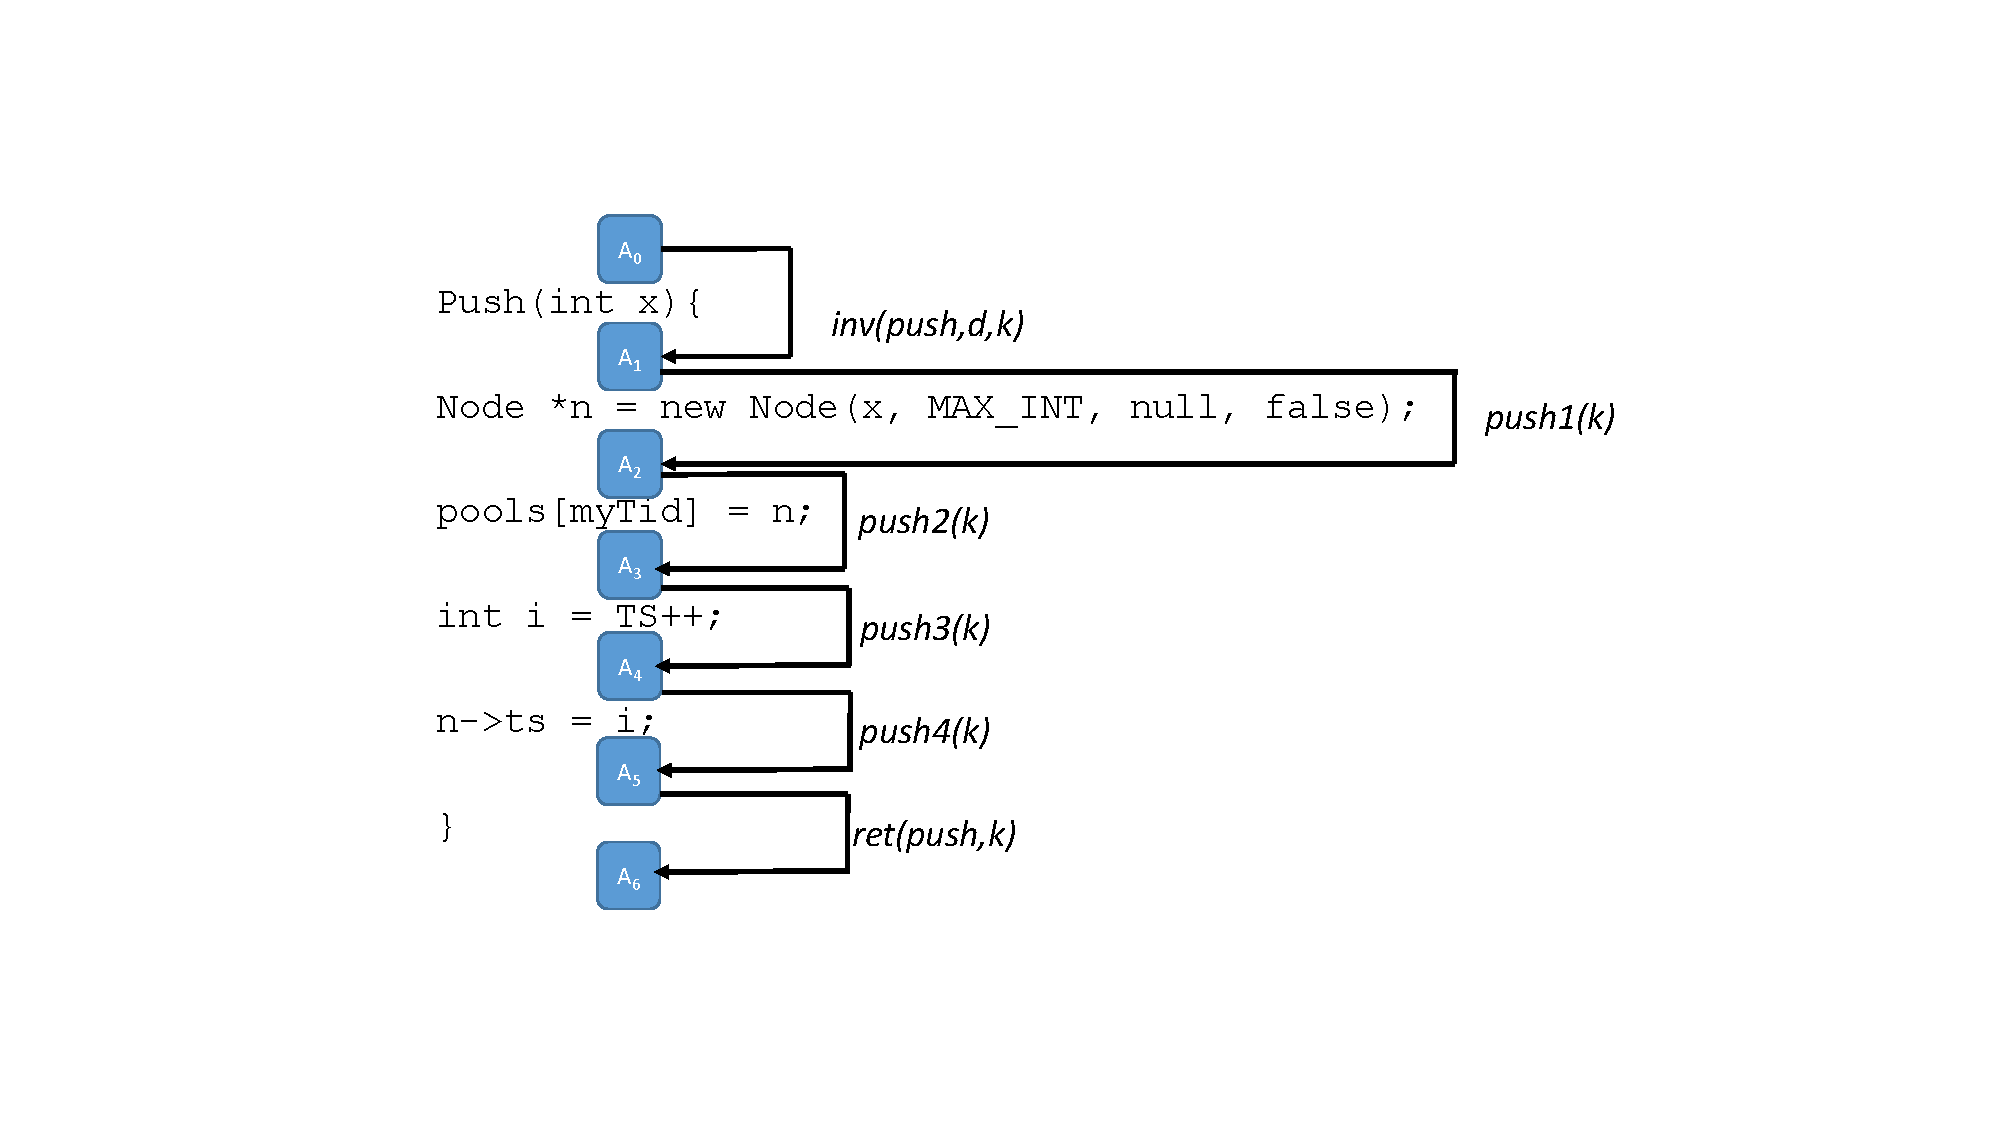
\includegraphics[width=7cm]{tssPushFlow.pdf}
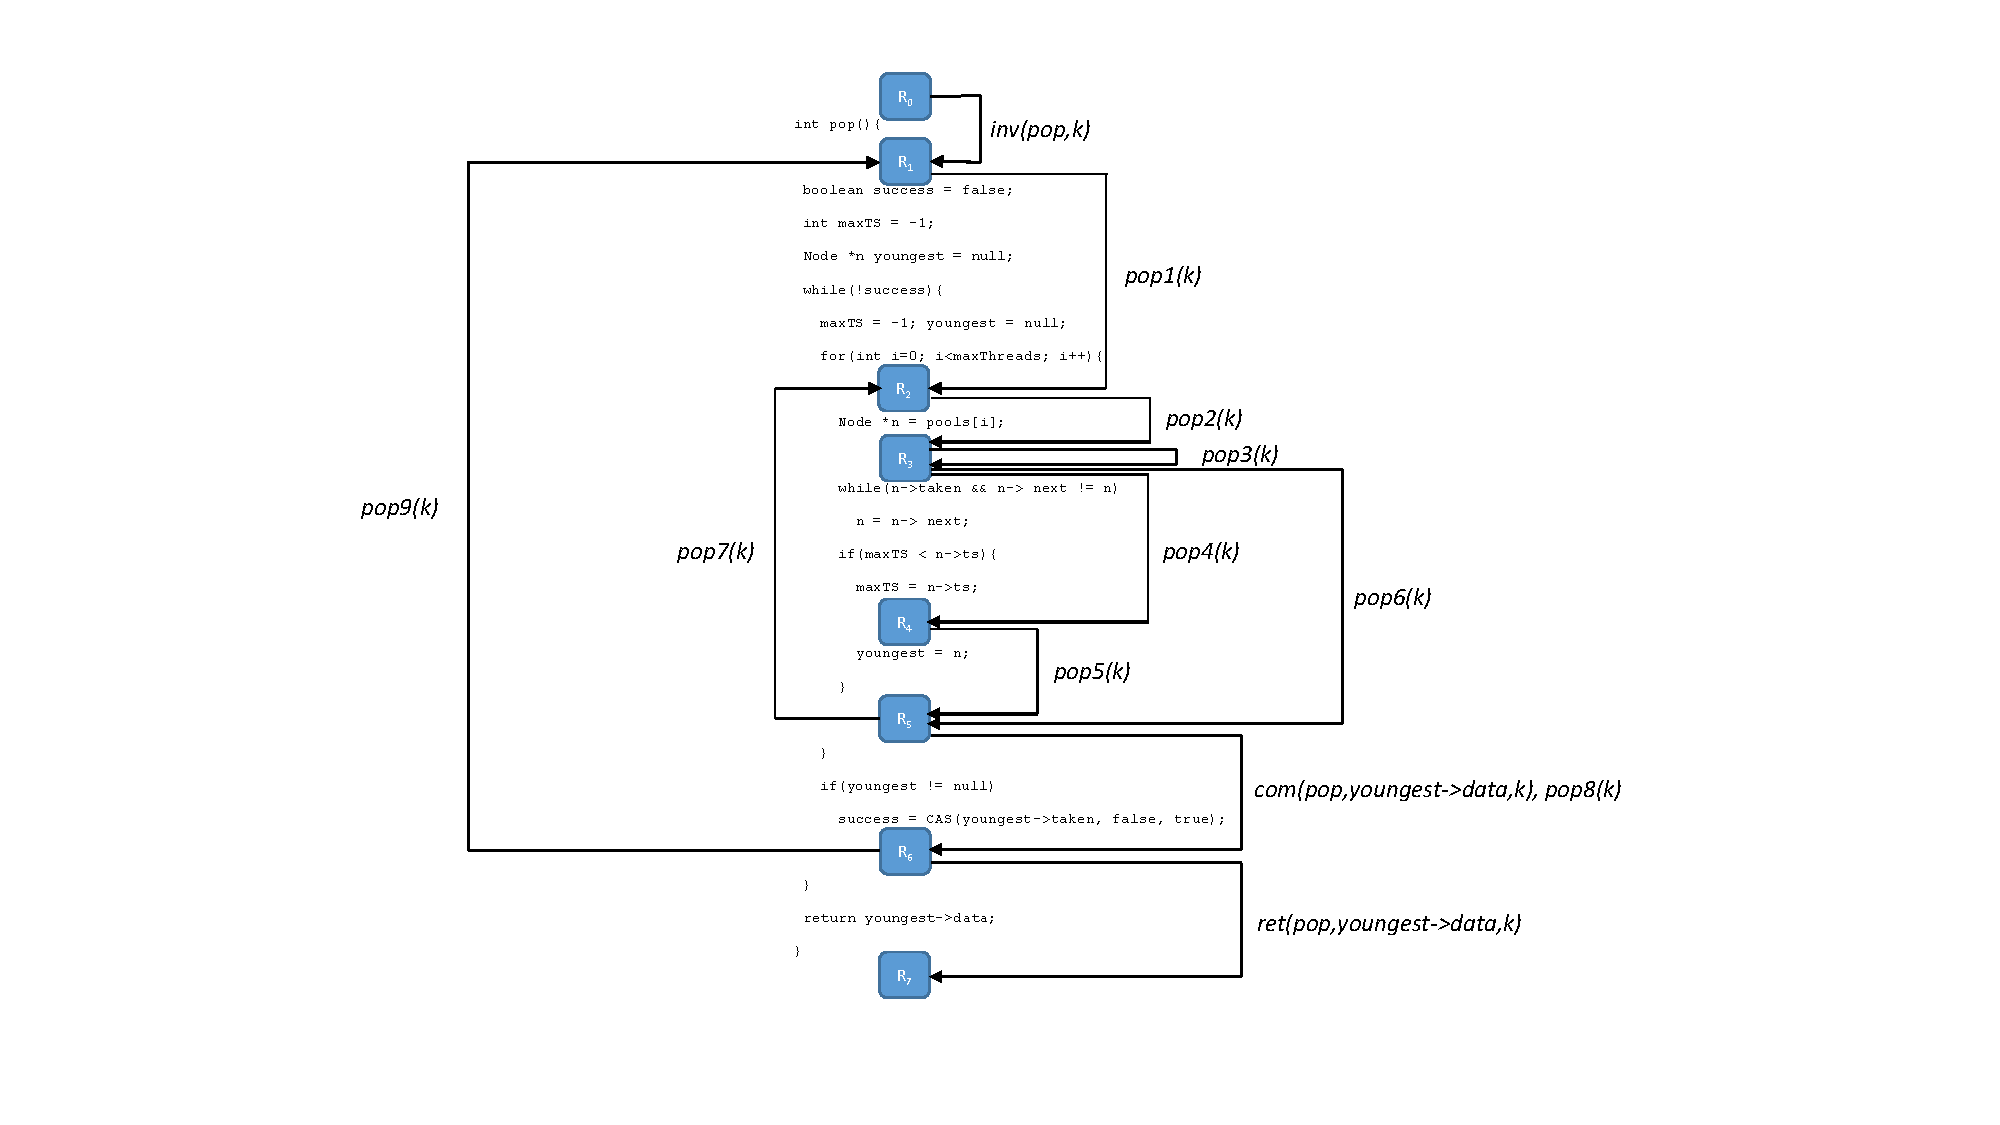
\includegraphics[width=16cm]{tssPopFlow.pdf}
\vspace{-8mm}
\caption{The flow diagram for the pop and push methods of the Time-Stamped Stack algorithm. The blue points show the control points roughly and the arrows show the possible transitions.}
\label{fig:tssFlow}
\end{figure}



The LTS corresponding to the description of $TSS$ given in Fig.~\ref{fig:TimeStamped} is defined as usual. The control points and transition labels we use in the following proof are pictured in Fig.~\ref{fig:tssFlow}. To simplify the proof, we take the initializations of some local variables together as atomic.

States of the TS-Stack contains the global variables and local variables as fields. Global variables are just elements of their domains and local variables are maps from operation identifiers to their domains. We say $i_q(k)$ for referencing the value of local variable $i$ of operation $k$ in state $q$. There is only one special local variable called $myTID$. Its value is unique to each pending operation in a state i.e., concurrent operations cannot have the same $myTID$ value. TS-Stack states also contains sets $O_a, O_r \in \mathbb{O}$ which are operation identifier sets of push and pops respectively, and the control point function $cp$ which is a map from operation identifiers to the control points set that are presented in the flow diagram Figure ~\ref{fig:tssFlow}. Transition relation of the TS-STack is presented in Figure~\ref{fig:transitions:TSSPush} (push rules) and Figure~\ref{fig:transitions:TSSPop} (pop rules).
Next, we show that the linearizability of TS Stack.

\begin{figure} [t]
{\scriptsize
  \centering
  \begin{mathpar}
    \inferrule[call-push]{
      k\not\in dom(cp) \\ 
      d\neq {\tt null}
    }{
      ..., O_a, x, cp,...
      \xrightarrow{inv(push,d,k)} 
     ..., O_a\cup\{k\}, x[k \mapsto d], cp[k \mapsto A_1], ...
    }\hspace{5mm}

    \inferrule[push1]{
      cp(k) = A_1 \\ 
      *n' = (x(k),\texttt{MAX\_INT}, \texttt{null}, \texttt{false})
    }{
      ..., n, cp,...
      \xrightarrow{push1(k)} 
     ..., n[k \mapsto n'], cp[k \mapsto A_2], ...
    }\hspace{5mm}
    
  
  \inferrule[push2]{
      cp(k) = A_2 
    }{
      ..., pools, cp,...
      \xrightarrow{push2(k)} 
     ..., pools[myTid(k) \mapsto n(k)], cp[k \mapsto A_3], ...
    }\hspace{5mm}
    
      \inferrule[push3]{
      cp(k) = A_3 
    }{
      ..., i, TS, cp,...
      \xrightarrow{push3(k)} 
     ..., i[k \mapsto TS], TS+1, cp[k \mapsto A_4], ...
    }\hspace{5mm}
    
   \inferrule[push4]{
      cp(k) = A_4 \\
      n'(k) = n(k)[ts \mapsto i(k)] \\
      \forall k'. cp(k') = A_6 \implies i(k') < i(k)
    }{
      ..., n, cp,...
      \xrightarrow{push4(k)} 
     ..., n[k \mapsto n'(k)], cp[k \mapsto A_5], ...
    }\hspace{5mm}
    
   \inferrule[ret-push]{
      cp(k) = A_5 
    }{
      ...,cp,...
      \xrightarrow{ret(push,k)} 
     ...,cp[k \mapsto A_6], ...
    }\hspace{5mm}
    
      \end{mathpar}
  }
 \vspace{-5mm}
  \caption{The push derivation rules of $TSS$. We only mention the state components that are modified. Unmentioned state components have the names in the algorithm in the prestate. $*n = (a,b,c,d)$ is shorthand for $n->data = a$, $n->ts = b$, ... $n' = n[ts \mapsto expr]$ is short for $n'->ts = expr$ and all the other fields of $n$ and $n'$ are the same.
  }
  \label{fig:transitions:TSSPush}
\vspace{-2mm}
\end{figure}

\begin{figure} [t]
{\scriptsize
  \centering
  \begin{mathpar}
    \inferrule[call-pop]{
      k\not\in dom(cp) 
    }{
      ..., O_r, cp,...
      \xrightarrow{inv(pop,k)} 
     ..., O_r\cup\{k\}, cp[k \mapsto R_1], ...
    }\hspace{5mm}
    
    \inferrule[pop1]{
      cp(k) = R_1 \\
      maxThreads > 0
    }{
      ..., suc, ygst, mTS, i, cp
      \xrightarrow{pop1(k)} 
     ..., suc[k \mapsto \texttt{false}], ygst[k \mapsto \texttt{null}], mTS[k \mapsto -1], i[k \mapsto 0],  cp[k \mapsto R_2]
    }\hspace{5mm}
    
    \inferrule[pop2]{
      cp(k) = R_2 \\
      0 \leq i(k) < \texttt{maxThreads}
    }{
      ..., n, cp, ...
      \xrightarrow{pop2(k)} 
     ..., n[k \mapsto pools(i(k))], cp[k \mapsto R_3],...
    }\hspace{5mm}
    
    \inferrule[pop3]{
      cp(k) = R_3 \\
      n(k) \neq \texttt{null}\\
      n(k)->taken = \texttt{true}\\
      n(k)->next \neq n(k)
    }{
      ..., n, ...
      \xrightarrow{pop3(k)} 
     ..., n[k \mapsto n(k)->next],...
    }\hspace{5mm}
    
    \inferrule[pop4]{
      cp(k) = R_3 \\
      n(k) \neq \texttt{null}\\
      n(k)->taken = \texttt{false}\\
      n(k)->ts > maxTS(k)
    }{
      ..., maxTS, cp ...
      \xrightarrow{pop4(k)} 
     ..., maxTS[k \mapsto n(k)->ts], cp[k \mapsto R_4]...
    }\hspace{5mm}
    
    \inferrule[pop5]{
      cp(k) = R_4 
    }{
      ..., youngest, cp ...
      \xrightarrow{pop5(k)} 
     ..., youngest[k \mapsto n(k)], cp[k \mapsto R_5]...
    }\hspace{5mm}
    
    \inferrule[pop6]{
      cp(k) = R_3 \\
      n(k) \neq \texttt{null}\\
      n(k)->taken = \texttt{false}\\
      n(k)->ts \leq maxTS(k)
    }{
      ..., cp, ...
      \xrightarrow{pop6(k)} 
     ...,cp[k \mapsto R_5],...
    }\hspace{5mm}
    
    \inferrule[pop7]{
      cp(k) = R_5 \\
      i(k) < \texttt{maxThreads}-1
    }{
      ...,i, cp, ...
      \xrightarrow{pop7(k)} 
     ...,i[k \mapsto i(k)+1], cp[k \mapsto R_2],...
    }\hspace{5mm}
    
    \inferrule[pop8]{
      cp(k) = R_5 \\
      youngest(k) = \texttt{null} \vee (youngest(k) \neq \texttt{null} \wedge youngest->taken)
    }{
      ...,success, cp, ...
      \xrightarrow{pop7(k)} 
     ...,success[k \mapsto \texttt{false}], cp[k \mapsto R_6],...
    }\hspace{5mm}
    
    \inferrule[com-pop]{
      cp(k) = R_5 \\
      youngest(k) \neq \texttt{null} \\
      youngest(k) = m \\
      d = m->data\\
      m->taken = false \\
      m' = m[taken \mapsto true]
    }{
      ...,success, youngest, cp, ...
      \xrightarrow{com(pop,d,k)} 
     ...,success[k\mapsto true], youngest[k \mapsto m'], cp[k \mapsto R_6],...
    }\hspace{5mm}
    
    \inferrule[pop9]{
      cp(k) = R_6 \\
      success(k) = \texttt{false}
    }{
      ..., cp, ...
      \xrightarrow{pop9(k)} 
     ..., cp[k \mapsto R_1],...
    }\hspace{5mm}
    \inferrule[ret-pop]{
      cp(k) = R_6 \\
      suc(k) = \texttt{false} \\ 
      d = yst(k)->data
    }{
      ..., cp, ...
      \xrightarrow{ret(pop,d,k)} 
     ..., cp[k \mapsto R_7],...
    }\hspace{5mm}
    
    


    \end{mathpar}
  }
 \vspace{-5mm}
  \caption{The pop derivation rules of $TSS$. We only mention the state components that are modified. Unmentioned state components have the names in the algorithm in the pre-state. $n' = n[taken \mapsto expr]$ is short for $n'->taken = expr$ and all the other fields of $n$ and $n'$ are the same.
  }
  \label{fig:transitions:TSSPop}
\vspace{-6mm}
\end{figure}

\begin{lem}
$TSS$ is a $C\cup R\cup Com(pop)$-refinement of $AbsS$. 
\end{lem}
\begin{proof}
We show that the relation $\mathit{fs}_2$ defined in Section~\ref{sec:corr_tss} is a $C\cup R\cup Com(pop)$-forward simulation  from $TSS$ to $AbsS$. For readability, we recall the definition of $\mathit{fs}_2$.

Let us make some clarifications before defining the relation. In order not to confuse nodes in TS Stack and nodes in $AbsS$, we call nodes of $AbsS$ as vertices from now on. We also define ordering relation (called traverse order) among the operations in a state of $TS$. It basically reflects the traverse order of pop operations. For two push operations $m,n \in O_a$ is state $s$ we say that $m <^{tr}_s n$ iff either $myTid(m) < myTid(n)$ or $myTid(m) = myTid(n)$ and $n_s(n)$ is reachable from $n_s(m)$ using next pointers. $\geq^{tr}$ is obtained from $<^{tr}$ in the usual way.

The relation $\mathit{fs}_2 \subseteq Q_C \rightarrow Q_{AbsS}$ contains $(s,t)$ iff the following are satisfied:
\begin{itemize}
\item[\emph{Nodes}] $k \in O_t$ iff $k$ is a push operation in $s$ ($k \in O_a$) such that either it has not inserted its node to the pool yet ( $cp_s(k) = A_i$ and $i<3$) or its node is not taken by a pop ($cp_s(k) = A_i$, $i\geq 3$ and $n_s(k)->taken = false$). 
\item[\emph{Pend/Comp}] A vertex $k \in O_t$ is pending ($\ell_t(k) = (d, \texttt{PEND})$) iff $k$ satisfies the previous condition, $x_s(k) = d$ and it is not completed in $s$ ($cp_s(k) = A_i$ and $i<6$). Similarly, this vertex is completed ($\ell_t(k) = (d, \texttt{COMP})$) iff $k$ satisfies the previous condition, $x_s(k) = d$ and it is completed in $s$ ($cp_s(k) = A_6$). Pending vertices are maximal with respect to $<_t$ i.e., if $k \in O_t$ is a pending vertex, then for all $k' \in O_t$ $k \nless_t k'$.
\item[\emph{TSOrder}] If a node has a smaller timestamp than the other node in $s$, the operations that inserted them cannot be ordered reversely in $t$. More formally, let $k, k' \in O_t$ s.t. $n_s(k)-> ts \leq n_s(k')->ts$. Then, $k' \nless_t k$.
\item[\emph{TidOrder}] Order among the nodes inserted by the same threads in $s$ must be preserved among the operations that inserted them in $t$. Let $k, k' \in O_t$ s.t. $myTid_s(k) = myTid_s(k')$ and $n_s(k)->ts < n_s(k')->ts$. Then, $k <_t k'$.
\item[Frontiers] Every maximally closed or pending vertex can be removed by a pending pop. More formally, let $k \in O_t$ such that $\ell_t(k) = (\_,\texttt{PEND})$. Then, for all pops $p$, $k \in ov_t(p)$. In the other case, let $k \in O_t$ such that $\ell_t(k) = (\_,\texttt{COMP})$ and for all other $k' \in O_t$ such that $k<_t k'$, we know $\ell_t(k') = (\_,\texttt{PEND})$. Then, for all pop operations $p$, $k \in be_t(p)$ or $k \in ov_t(p)$. 
\item[\emph{MaximalOV}] If a push $k \in O_t$ is a candidate to be removed by a pop $p$, then every other push $k'$ invoked after $k$ is a candidate to be removed by $p$ since $k$ is concurrent with $p$. More formally, let $k, k' \in O_t$ such that $k <_t k'$ and there exists a pop $p$ such that $k \in be_t(p)$ or $k \in ov_t(p)$. Then, $k' \in ov_t(p)$.
\item[\emph{MinimalBE}] If a push $k \in O_t$ has finished before the pop $p$ is invoked and yet $k$ is a candidate to be removed by $p$, other pushes completed before $k$ can not be candidates to be removed by $p$ at that state. More formally, let $k, k' \in O_t$ such that $k <_t k'$ and there exists a pop $p$ such that $k' \in be_t(p)$. Then, neither $k \in be_t(p)$ nor $k \in ov_t(b)$.
\item[\emph{ReverseFrontiers}] If all immediate followers $k' \in O_t$ of a push $k \in O_t$ are concurrent with pop $p$, then $k$ is either concurrent or maximally closed with respect to $p$. More formally, let $k \in O_t$ and for all $k' \in O_t$ such that $k \in pred_{<_t}(k')$, $k' \in ov_t(p)$, where $p$ is a pop operation. Then, $k \in ov_t(p) \cup be_t(p)$. 
%If a push $k \in O_t$ is concurrent with the pop $p$ and there exists another push $k' \in O_t$ that is immediate predecessor of $k$, then $k'$ is either concurrent or maximally closed with respect to $p$. More formally, let $k, k' \in O_t$ such that $k' \in pred_{<_t}(k)$ and $k \in ov_t(p)$ for some pop $p$. Then, either $k' \in ov_t(p)$ or $k' \in be_t(p)$. 
\item[\emph{FixReturn}] If a pop $p$ is after its commit point action in $s$, then the $rv$ value of this operation in $t$ is fixed to $youngest_s(p)->data$. More formally, Let $p$ be the pop operation such that $cp_s(p) = R_6$ and $success_s(p) = \texttt{true}$. Then, $rv_t(p) = youngest_s(p)->data$. 
\item[\emph{TraverseBefore}] If a pop operation $p$ is currently visiting node $n$, it has non-null node $y$ as the $youngest$ and there is a non-null not taken node $m$ coming before $n$ in the traverse order with a greater timestamp than $y$, then the operation that inserts $m$ must be concurrent with $p$. More formally, assume $youngest_s(p) = y$ and $ y \neq \texttt{null}$. Let $k \in O_t$ such that $n_s(k) \neq \texttt{null}$, $n_s(k)->taken = \texttt{false}$, $n_s(k) <^{tr}_s n_s(p)$ and $n_s(k)->ts \geq y->ts$. Then, $k \in ov_t(p)$.
\item[\emph{TraverseBeforeNull}] If a pop operation $p$ is currently visiting node $n$, and its $youngest$ field is \texttt{null}, then every other node $m$ coming before $n$ in the traverse order must be concurrent with $p$. More formally , let $youngest_s(p) = \texttt{null}$ and assume there exists  an operation $k \in O_t$ such that $n_s(k) \neq \texttt{null}$, $n_s(k)->taken = \texttt{false}$ and  $n_s(k) <^{tr}_s n_s(p)$. Then, $k \in ov_t(p)$. 
\item[\emph{TraverseAfter}] If a pop operation $p$ is currently visiting node $n$ that is not null and its youngest element $m$ is not null and still not taken in state $s$, then either $m$ is a candidate to be removed by $p$ in $t$ or there exists a later node $m'$ than $n$ such that $m'$ is a candidate in $t$ and it has a bigger timestamp than n. More formally, assume that there exists $k, k' \in O_t$ such that $youngest_s(p)->taken \neq false$, $youngest_s(p) = n_s(k)$ and $n_s(k') = n_s(p)$. Then, either $k \in ov_t(p) \vee k \in be_t(p)$ or there exists $k'' \in O_t$ s.t. $n_s(k'')->ts > n_s(k) ->ts$ and $k'' \in ov_t(p) \vee k'' \in be_t(p)$ and either $k' <^{tr}_s k''$ or $n_s(p) = n_s(k'') \wedge cp_s(p) = R_j \wedge j<5$. 
\end{itemize}
Next, we will show that $\mathit{fs}_2$ is really a $C\cup R\cup Com(pop)$-forward simulation relation. Except the trivial base case, we case-split on the transition rules. We first assume $s \xrightarrow{\alpha}_{TSS} s' $ and $t \in \mathit{fs}_2[s]$. Then, we find  corresponding transition $\alpha' \in \Sigma_{AbsS}$ obeying the $C\cup R\cup Com(pop)$-forward simulation relation conditions and obtain $t'$ such that $t \xrightarrow{\alpha'}_{AbsS} st $  and $t' \in \mathit{fs}_2[s']$.

We observe that if $\alpha \in C \cup R \cup Com(pop)$, then the corresponding rule in $AbsS$ is $\alpha' = \alpha$. Otherwise, $\alpha' = \epsilon$.

Let the following describe $\alpha$: $\psi \triangleright s\xrightarrow{\alpha}_{TSS} s'$ where $\psi$ is the precondition (guard) that needs to be satisfied for enabling $\alpha$ and $\psi' \triangleright t \xrightarrow{\alpha'}_{AbsS} t'$ describe the $\alpha'$ if $\alpha' \neq \epsilon$ (equivalently $\alpha' = \alpha$).

For the cases $\alpha' = \alpha$, we first need to show $\alpha'$ is enabled in state $t$ i.e., $t$ satisfies $\psi'$. If this can not be directly obtained from the information that $s$ satisfies $\psi$ and using one or two obvious conditions on $\mathit{fs}_2$ (since $t \in \mathit{fs}_2[s]$), we show the derivation in the proof. Then, $t'$ is obtained in a unique way since $AbsS$ is deterministic on its alphabet $ \Sigma_{AbsS} = C \cup R \cup Com(pop)$. The, only other thing to show is $t' \in \mathit{fs}_2[t']$. We show this by proving that $t'$ does not violate any of the conditions of the $\mathit{fs}_2$ described above. Suppose conditions on $\mathit{fs}_2$ are of the form $\forall \overline{k}. guard_{s,t}(\overline{k}) \triangleright \phi_{s,t}(\overline{k})$ where the $\overline{k}$ is a vector of operation identifiers and $\phi$ defined on states $s$ and $t$ must hold if the guard defined on $s$ and $t$ holds. We say that a vector $\overline{k_1}$ is a new instantiation of the condtion if $\overline{k_1}$ does not satisfy the $guard_{s,t}$ while relating pre-states, but it satisfies $guard_{s',t'}$ while relating post-states.

We only explain why the new instantiations due to the difference between $s'$ and $s$ or the difference between $t'$ and $t$ do not violate the conditions. We skip the instances that we assumed while relating $s$ to $t$.

For the cases in which $\alpha' = \epsilon$, we have $t'=t$ and the only thing to show is $t \in \mathit{fs}_2[s']$. Again, we only explain why the new instantiations due to the difference between $s'$ and $s$ do not violate the conditions.

In the following, we show that $\mathit{fs}_2$ is a $C \cup R \cup Com(pop)$-forward simulation relation.
\begin{itemize}
\item[\textsc{init}] $\mathit{fs}_2[{q_0}_{TSS}] =\{{q_0}_{AbsS}\}$
\item[\textsc{call-push}] The same derivation rule of $TSS$ is applied to $t$  to obtain $t'$. The premise of the rule is satisfied by $t$ trivially in the sense explained before. The new vertex $k$ is added to the $O_t$ such that $k$ is maximal, pending and every completed vertex is ordered before $k$ in $t'$. Moreover, $k$ is overlapping with every pending pop. To see that $t' \in \mathit{fs}_2[s']$ we observe the following: \emph{Nodes} condition is preserved because $k \in O_{t'}$. Since the newly added vertex $k$ is maximal and pending in $t'$, \emph{Pend/Comp} condition is preserved. \emph{Frontiers} and \emph{MaximalOV} conditions are not violated since $k$ is added to $ov(p)$ set for every pending pop operation $p$. 
\item[\textsc{push1}] We have $t' = t$ and show $t \in \mathit{fs}_2[s']$.\emph{Nodes} and \emph{Pend/Comp} conditions are still satisfied since $k$ remains to be a pending vertex. \emph{TSOrder} is still preserved. Timestamp of $n_{s'}(k)$ is maximal and every other nodes of push operations with maximal timestamp in $s'$ are pending vertices in $t$. Hence there can be no ordering between those pushes and $k$ in $t$ that can violate \emph{TSOrder}. Moreover, $k$ is maximal in $t$ which means that it cannot be ordered before another push $k'$ of which node has a lower timestamp. \emph{TidOrder} is also satisfied. Since $k$ is ordered after every completed push in $t$ and every other push by the same thread is completed, ordering required by the \emph{TidOrder} is present.
\item[\textsc{push2}] We have $t' = t$ and show $t \in \mathit{fs}_2[s']$. \emph{Nodes} and \emph{Pend/Comp} conditions are still satisfied since $k$ remains to be a pending vertex. One can also see that the \emph{TraverseBefore} condition is preserved. Let the pop $p$ visiting node $m$ and $n_{s'}(k) <^{tr}_{s'} m$. Since $k$ and $p$ are both pending in $s$ and $t \in \mathit{fs}_2[s]$, $k \in ov_t(p)$ (by the \emph{Frontiers} condition). Hence, \emph{TraverseBefore} is preserved. 
\item[\textsc{push3}] We have $t' = t$ and show $t \in \mathit{fs}_2[s']$. We consider two cases: $n_s(k)->taken$ is \texttt{true} or it is \texttt{false}. For the former case, $k \notin O_t$. The only new instantiation we check is $k \notin O_t$ does not violate \emph{Nodes} condition while relating $s'$ to $t$. 

For the latter case, we have $k \in O_t$. \emph{Nodes} and \emph{Pend/Comp} conditions are still satisfied since $k$ remains to be a pending vertex after changing $s$ to $s'$.
\item[\textsc{push4}] We have $t' = t$ and show $t \in \mathit{fs}_2[s']$. 

We consider two cases: $n_s(k)->taken$ is \texttt{true} or it is \texttt{false}. For the former case, \emph{Nodes} condition is still satisfied since $k$ remains to be not a vertex. 

For the latter case \emph{Nodes} and \emph{Pend/Comp} conditions are still satisfied since $k$ remains to be a pending vertex. \emph{TSOrder} condition is still not violated since if $k'<_t k$, then $k'$ is a completed vertex in $s$ and $s'$. By the premise of the rule (which can be shown to hold for every operation at control point $A_4$) $i_s(k') < i_s(k)$ and consequently $n_{s'}(k')->ts < n_{s'}(k)->ts$. Since every other push by the thread of $k$ is completed, \emph{TidOrder} still continues to hold for the same reasons. \emph{TraverseAfter} condition is also preserved. Let $k'$ be the push and $p$ be the pop such that $n_s(k') = youngest_s(p)$, $n_s(k') \leq^{tr}_s n_s(k)$, $n_s(k')->ts < n_s(k)->ts$ and $k \in ov_t(p)$ or $k \in be_t(p)$. Assume $n_{s'}(k')->ts \geq N_{s'}(k)->ts$ after the action. Then, $k'$ must be a pending push both in $s$ and $s'$ by the premise of the derivation rule and $k' \in ov_t(p)$ must be true by \emph{Frontiers} condition and $t \in \mathit{fs}_2[s]$. Hence, the \emph{TraverseAfter} condition is preserved.
\item[\textsc{ret-push}] We consider two cases, $n_s(k)->taken$ is \texttt{false} or \texttt{true}. For the former case, we obtain $t'$ by applying \textsc{ret-push1} rule of $AbsS$. \emph{Nodes} and \emph{Pend/Comp} conditions are still satisfied since $k$ becomes a completed vertex in $t'$. \emph{Frontiers} condition still holds since although $k$ become a maximally closed vertex in $t'$, we have $k \in ov_{t'}(p)$ for all pending nodes $p$ (due to \emph{Frontiers} condition, $t \in \mathit{fs}_2[s]$ and $k$ was a pending operation in state $t$, $k \in ov_t(p)$). 

For the latter case, we obtain $t'$ by applying \textsc{ret-push2} rule of $AbsS$. \emph{Nodes} condition is still satisfied since $k \notin O_{t'}$. 
\item[\textsc{call-pop}] The same derivation rule of $TSS$ is applied to $t$  to obtain $t'$. \emph{Frontiers} condition holds for $p = k$ relating $s'$ to $t'$ since $k' \in ov_{t'}(k)$ for every pending vertex $k'$ and $k'' \in be_{t'}(p)$ for all completed vertex $k''$. $t'$ due to action $inv(pop,k)$ applied on $t$. \emph{MaximalOV} condition holds for $p = k$ since pending vertices are maximal in $t'$ and for any maximally closed vertex $k'$ in $t'$, if $k'$ is ordered before other vertex $k''$, then $k''$ is a pending operation by definition of being maximally closed and $k'' \in ov_t(k)$ due to the changes by \textsc{inv-pop} action on $t$. \emph{MinimalBE} condition holds while relating $s'$ to $t'$ for the pop $ p = k$ because only maximally closed vertices are in $be(k)$ and if a push $k'$ is ordered before a maximally closed push $k''$ in $t$, neither $k'' \in be_{t'}(k)$ (since $k''$ is not maximally closed) nor $k'' \in ov_{t'}$ (since $k''$ cannot be pending). \emph{ReverseFrontiers} condition holds while relating $s'$ to $t'$ for the pop $p=k$ because, if $k'' \in ov_{t'}(k)$ for all immediate successors of $k'$ in $t$, then $k'' $ are pending vertices (due to \emph{call-pop} action of $AbsS$), $k'$ is a maximally closed vertex and $k' \in be_{t'}(k)$ (due to \emph{call-pop} action of $AbsS$).
\item[\textsc{pop1}]We have $t' = t$ and $t \in \mathit{fs}_2[s']$.
\item[\textsc{pop2}]We have $t' = t$ and show $t \in \mathit{fs}_2[s']$. \emph{TraverseBefore} condition while relating $s'$ to $t$ still holds for $p=k$. Assume $youngest_{s'}(k) = y$ is a non-null node. Then, for all nodes $m$ in $s'$ such that $n_s(k) \leq^{tr}_{s'} m <^{tr}_{s'} n_{s'}(k)$ we have $m->ts < y->ts$ in $s'$ because  $n_s(k)->ts > m->ts$ (since $n_s(k)$ is added to the pool after $m$ by the same thread) and $y->ts \geq n_s(k)->ts$ in $s'$ (since either $youngest_{s'}(k) = n_s(k)$ or $youngest_{s'}(k)->ts > n_s(k)->ts$). \emph{TraverseAfter} does not have any new instatiations since the guard mentions the nodes after $n_s(k)$ while relating $s$ to $t$ whereas it mentions nodes after or including $n_{s'}(k)$ which contains the all nodes in the former case.
\item[\textsc{pop3}]We have $t' = t$ and $t \in \mathit{fs}_2[s']$.
\item[\textsc{pop4}]We have $t' = t$ and $t \in \mathit{fs}_2[s']$.
\item[\textsc{pop5}]We have $t' = t$ and show $t \in \mathit{fs}_2[s']$. 
\emph{TraverseBefore} condition while relating $s'$ to $t$ still holds for $p=k$ since $youngest_s(k)->ts < youngest_{s'}(k)->ts$ and \emph{TraverseBefore} holds while relating $s$ to $t$. 

\emph{TraverseAfter} condition also continues to hold for $p=k$. There are two possible cases: $youngest_s(k) = \texttt{null}$ or not. 

First, consider the former case. Since \emph{TraverseBeforeNull} is satisfied while relating $s$ to $t$, for every operation $k', k'' \in O_t$ such that  $k'' <^{tr}_s k'$ and $n_s(k') = youngest_{s'}(k)$ we have $k'' \in ov_t(k)$. Consider all such $k''$ such that $n_s(k'')->ts > n_s(k')->ts$. If there exists such a $k''$ such that $k' \in pred_{<_t}(k'')$, then $k' \in ov_t(k) \cup be_t(k)$ since \emph{ReverseFrontiers} condition holds relating $s$ to $t$. Otherwise, either $k'$ is maximal in $t$ or all the vertices $v$ ordered after $k'$ in $t$ we have $v >^{tr}_s k'$. Then, either $k'$ or one of these $v$ vertices must be maximal in $t$ and must be in $be_t(k) \cup ov_t(k)$ since \emph{Frontiers} condition holds (one of them is maximal in $t$) while relating $s$ to $t$. 

Second, assume there exists push operations $j, k'$ such that $n_s(j) = youngest_s(k) \neq \texttt{null}$ and $n_s(k') = n_s(k) = youngest_{s'}(k)$ . Since \emph{TraverseBefore} is satisfied while relating $s$ to $t$, if there exists a push $k'' <^{tr}_s k'$ such that $n_s(k'')$ is not taken and $n_s(k'')->ts \geq n_s(j)->ts$, then $k'' \in ov_t(k)$. Then, for all $k'' <^{tr}_s k'$ such that $n_s(k'')$ is not taken and $n_s(k'')->ts \geq n_s(k')->ts$, then $k'' \in ov_t(k)$ since $n_s(k')->ts \geq n_s(j)->ts$. If there exists such a $k''$ such that $k' \in pred_{<_t}(k'')$, then $k' \in ov_t(k) \cup be_t(k)$ since \emph{ReverseFrontiers} condition holds relating $s$ to $t$. Otherwise, either $k'$ is maximal in $t$ or all the vertices $v$ ordered after $k'$ in $t$ we have $v >^{tr}_s k'$. Then, either $k'$ or one of these $v$ vertices must be maximal in $t$ and must be in $be_t(k) \cup ov_t(k)$ since \emph{Frontiers} condition holds (one of them is maximal in $t$) while relating $s$ to $t$. 

\item[\textsc{pop6}] We have $t' = t$ and show $t \in \mathit{fs}_2[s']$. \emph{TraverseAfter} continues to hold while relating $s'$ to $t$ for $p=k$. Let $k', k'' \in O_t$ such that $youngest_s(k) = n_s(k')$, $n_s(k) = n_s(k'')$ and $k' \notin  ov_t(k) \cup be_t(k)$. Note that $k' <^{tr}_s k''$. Then, $n_s(k'')->ts < n_s(k')->ts$ since $n_s(k'')->ts < maxTS(k)$ and $maxTS(k) = n_s(k')->TS$ ($n_s(k')->ts$ cannot be \texttt{MAX\_INT} since $k'$ would be pending and $k' \in ov_t(k)$ otherwise). Hence, there exists another push $j$ such that $j >^{tr}_s$ and $j \in ov_t(k) \cup be_t(k)$. 

\item[\textsc{pop7}] We have $t' = t$ and $t \in \mathit{fs}_2[s']$.
\item[\textsc{pop8}] We have $t' = t$ and $t \in \mathit{fs}_2[s']$.
\item[\textsc{com-pop}] $t'$ is obtained by applying \textsc{com-pop1} rule of $AbsS$.
We first show that precondition of \textsc{com-pop1} rule of $AbsS$ si satisfied by $t$. If $com(pop,d,k)$ removes a  node $n$ such that there exists a push $k'$ such that $n_s(k') =n$ in $s$, then $k' \in O_t$ since it is non-null and not taken. Moreover, $k' \in ov_t(k) \cup be_t(k)$ since \emph{TraverseAfter} is preserved while relating $s$ to $t$ and all the nodes that come after $n_s(k)$ in terms of traverse order in $s$ have lower timestamp values than $n_s(k)->ts$ and $n_s(k)->ts \leq youngest_s(k)->ts$.

Next, we show that $t' \in \mathit{fs}_2[s']$. We case split on the conditions of $\mathit{fs}_2$ considering new instantiations.

\emph{Nodes} condition is still preserved after $k$ removes the node pushed by operation $k'$ in $s$ since $k' \notin O_{t'}$ anymore by due to $com(pop,d,k)$ action. 

\emph{Frontiers} condition is still preserved if $k$ removes the vertex $k'$ and makes another $k''$ maximally closed in $t$. Since all the other nodes $j$ ordered after $k''$ (except possibly $k'$) in $t$ are pending, $j \in ov_t(p)$ (due to \emph{Frontiers} condition while relating $s$ to $t$) for some pending pop $p \neq k$. Then, $k'' \in be_{t'}(p)$ by $com(pop,d,k)$ action. 

For the \emph{MinimalBE} condition, we do not have a new instance. If $k' \in be_{t'}(p)$ becomes true although $k' \notin be_t(p)$, we cannot have $k'' \in O_{t'}$ such that $k' \in pred_{<_{t'}}(k'')$ and $k'' \in be_{t'}(p)$ since $com(pop,d,k)$ does not add $k''$ to $ov(p)$ if its successor is not pending with respect to $p$.

\emph{ReverseFrontiers} condition is still preserved. If $k$ removes the vertex $k'$ and there exists an immediate predecessor $k''$ of $k'$ such that all of immediate successors of $k''$ are in $ov_{t'}(p)$, then $k'' \in ov_{t'}(p)$ due to the action $com(pop,d,k)$.

\emph{TraverseAfter} condition is still preserved after $k$ removes the node of push $k'$. Let $p \neq k$ be another pop operation such that $n_s(j) = youngest_s(p)$ for some push $j$ and $n_s(k')$ be the only node such that $n_s(k')->ts > youngest_s(p)->ts$ and $n_s(k')$ comes after $n_s(p)$ in the traverse order of $s$ and $k' \in ov_t(p) \cup be_t(p)$. Hence, there is no $k''$ such that $n_s(k'')$ comes after $n_s(p)$ in the traverse order and $j <_t k''$ except $k'$ (i). In other direction, if for all $k'' \in O_t$ such that $n_s(k'')$ comes before $n_s(p)$ in the traverse order and $n_s(k'')->ts > youngest_s(p)->ts$ , then $k'' \in ov_t(p)$ since \emph{TraverseBefore} condition holds while relating $s$ to $t$. Then, for all $k'' \in O_t$ such that $n_s(k'')$ comes before $n_s(p)$ in the traverse order of $s$ and $k'' >_t j$ implies $k'' \in ov_t(p)$ since $n_s(k'')->ts > n_s(j)->ts$ if $k'' >_t j$ (ii). Then, for all $k'' \in O_t$ such that if $k'' >_t j$, then $k'' \in ov_t(p)$ except $k'$ due to (i) and (ii). If $j \nless_t k'$, then $j \in ov_t(p) \cup be_t(p)$ since \emph{ReverseFrontiers} hold while relating $s$ to $t$ and $j \in ov_{t'} \cup be_{t'}$ after applying the action $com(pop,d,k)$. Otherwise, if $j <_t k'$, then $k \in be_{t'}$ after applying $com(pop,d,k)$.

\emph{FixReturn} condition continues to hold. If $com(pop,d,k)$ removes the node pushed by $k'$ in $s$, then $com(pop,d,k)$ removes the vertex $k'$ (assuming data independece) and $youngest_s(k')->data = \ell_t(k')_1$. Then, $youngest_{s'}(p)->data = rv_{t'}(p)$ after applying commit actions at both sides.

\item[\textsc{pop9}]We have $t' = t$ and $t \in \mathit{fs}_2[s']$.
\item[\textsc{ret-pop}] $t'$ is obtained by applying \textsc{ret-pop} rule of $AbsS$ and $t' \in \mathit{fs}_2[s']$.
\end{itemize}
\end{proof}
%\textcolor{red}{TODO: Check ReverseFrontiers for the cases before compop.}
%\textcolor{red}{TODO: Check TraverseBefore for the cases before pop2.}
%\textcolor{red}{TODO: CheckTraverseBeforeNull for the cases befoere pop 5.}
%\textcolor{red}{TODO: Apply Dr. Enea's comments.}
%\textcolor{red}{TODO: Try case split on fs conditions instantiations check.}

\end{document}
